%============================================================
%  MÉMOIRE D'INGÉNIEUR EN DATA SCIENCES
%  Université de Maroua — ENSPM
%  Auteur : NDZESSA AVELE BRUNO LANDRY
%============================================================

\documentclass[12pt, a4paper, oneside]{report}

%------------------------------------------------------------
%  ENCODAGE & LANGUE
%------------------------------------------------------------
\usepackage[utf8]{inputenc}
\usepackage[T1]{fontenc}
\usepackage[french]{babel}
\usepackage{csquotes}
\usepackage{booktabs}
\usepackage{siunitx}
\usepackage{float}
\usepackage{caption}
\usepackage[table]{xcolor}
%------------------------------------------------------------
%  POLICES & TYPOGRAPHIE
%------------------------------------------------------------
\usepackage{lmodern}
\usepackage{microtype}
\usepackage{setspace}
\onehalfspacing

%------------------------------------------------------------
%  GÉOMÉTRIE DE LA PAGE
%------------------------------------------------------------
\usepackage[
top=2.5cm,
bottom=2.5cm,
left=3cm,
right=2.5cm,
headheight=28pt        % CORRECTION 1 : 15pt → 28pt (évite le warning fancyhdr)
]{geometry}

%------------------------------------------------------------
%  EN-TÊTES & PIEDS DE PAGE
%------------------------------------------------------------
\usepackage{fancyhdr}
\pagestyle{fancy}
\fancyhf{}
\fancyhead[L]{\small\textit{\leftmark}}
\fancyhead[R]{\small\textit{ENSPM — Maroua}}
\fancyfoot[C]{\thepage}
\renewcommand{\headrulewidth}{0.4pt}
\renewcommand{\footrulewidth}{0pt}

\fancypagestyle{plain}{
	\fancyhf{}
	\fancyfoot[C]{\thepage}
	\renewcommand{\headrulewidth}{0pt}
}
%------------------------------------------------------------
%  COULEURS — VERSION IMPRESSION NOIR ET BLANC
%------------------------------------------------------------
\usepackage[dvipsnames, table]{xcolor}

% Remplace les couleurs vives par du noir et des gris
\definecolor{primary}{RGB}{0, 0, 0}          % noir pur → titres, cadres
\definecolor{secondary}{RGB}{80, 80, 80}     % gris foncé → sous-titres, filets
\definecolor{accent}{RGB}{50, 50, 50}        % gris très foncé → alertes
\definecolor{lightgray}{RGB}{240, 240, 240}  % gris clair → fonds de boîtes
\definecolor{darkgray}{RGB}{60, 60, 60}      % gris foncé → numéros de lignes
%------------------------------------------------------------
%  GRAPHIQUES & FIGURES
%------------------------------------------------------------
\usepackage{graphicx}
\usepackage{float}
\usepackage{subcaption}
\usepackage{wrapfig}
\usepackage{tikz}
\usetikzlibrary{shapes, arrows.meta, positioning, calc, decorations.pathmorphing}

%------------------------------------------------------------
%  TABLEAUX
%------------------------------------------------------------
\usepackage{booktabs}
\usepackage{tabularx}
\usepackage{multirow}
\usepackage{longtable}
\usepackage{array}

%------------------------------------------------------------
%  MATHÉMATIQUES & CODE
%------------------------------------------------------------
\usepackage{amsmath, amssymb, amsthm}
\usepackage{listings}
\usepackage{algorithm}
\usepackage{algpseudocode}

\lstset{
	basicstyle=\small\ttfamily,
	backgroundcolor=\color{lightgray},
	frame=single,
	framerule=0.5pt,
	rulecolor=\color{secondary},
	breaklines=true,
	numbers=left,
	numberstyle=\tiny\color{darkgray},
	keywordstyle=\color{primary}\bfseries,
	commentstyle=\color{darkgray}\itshape,
	stringstyle=\color{accent},
	captionpos=b,
	xleftmargin=2em,
	xrightmargin=0.5em,
	extendedchars=true,           % CORRECTION 2 : autorise les accents dans lstlisting
	inputencoding=utf8,
	literate=
	{é}{{\'e}}1 {è}{{\`e}}1 {ê}{{\^e}}1 {ë}{{\"e}}1
	{à}{{\`a}}1 {â}{{\^a}}1 {ä}{{\"a}}1
	{ù}{{\`u}}1 {û}{{\^u}}1 {ü}{{\"u}}1
	{î}{{\^i}}1 {ï}{{\"i}}1
	{ô}{{\^o}}1 {ö}{{\"o}}1
	{ç}{{\c{c}}}1 {œ}{{\oe}}1 {æ}{{\ae}}1
	{É}{{\'E}}1 {È}{{\`E}}1 {Ê}{{\^E}}1
	{À}{{\`A}}1 {Â}{{\^A}}1
	{Ç}{{\c{C}}}1,
}

%------------------------------------------------------------
%  HYPERLIENS & PDF METADATA
%  IMPORTANT : hyperref doit toujours être chargé AVANT biblatex
%------------------------------------------------------------
\usepackage[
colorlinks=true,
linkcolor=black,       % ← était primary (bleu)
citecolor=black,       % ← était secondary (bleu clair)
urlcolor=black,        % ← était secondary
bookmarks=true,
pdfauthor={NDZESSA AVELE BRUNO LANDRY},
pdftitle={Plateforme gouvernementale pour la cartographie et mise en relation
	des besoins des entreprises locales},
pdfsubject={Mémoire de fin d'études — Ingénieur en Data Sciences},
pdfkeywords={Data Sciences, Cartographie, Entreprises, MINEPAT, Cameroun}
]{hyperref}
%------------------------------------------------------------
%  BIBLIOGRAPHIE
%  CORRECTION 3 : style=apa nécessite le package biblatex-apa
%  installé via MiKTeX Package Manager
%------------------------------------------------------------
%\usepackage[backend=biber,natbib=true, style=ieee, citestyle=ieee]{biblatex}
 % Ton fichier de références
\usepackage[numbers]{natbib}
%\addbibresource{references.bib}
\bibliographystyle{plainnat}
%------------------------------------------------------------
%  PERSONNALISATION DES CHAPITRES
%------------------------------------------------------------
\usepackage{titlesec}

\titleformat{\chapter}[display]
{\normalfont\bfseries\color{black}}        % ← était color{primary}
{%
	\hfill
	\tikz[remember picture]{
		\node[fill=black, text=white,           % ← fill était primary
		font=\Large\bfseries,
		minimum width=1.5cm, minimum height=1.5cm,
		rounded corners=4pt]
		{\thechapter};
	}
}
{0pt}
{\vspace{1ex}\huge\raggedright}
[\vspace{0.5ex}{\color{black}\rule{\linewidth}{2pt}}]  % ← était primary

\titleformat{\section}
{\normalfont\large\bfseries\color{black}}  % ← était primary
{\thesection}{1em}{}
[\vspace{-0.5ex}{\color{darkgray}\rule{\linewidth}{0.6pt}}]  % ← était secondary

\titleformat{\subsection}
{\normalfont\normalsize\bfseries\color{black}}   % ← était secondary
{\thesubsection}{1em}{}

\titleformat{\subsubsection}
{\normalfont\normalsize\itshape\color{darkgray}} % ← était darkgray, ok
{\thesubsubsection}{1em}{}

%------------------------------------------------------------
%  TABLE DES MATIÈRES
%------------------------------------------------------------
\usepackage{titletoc}
\usepackage[titles]{tocloft}
\renewcommand{\cftchapfont}{\bfseries\color{black}}
\renewcommand{\cftchappagefont}{\bfseries\color{black}}
\renewcommand{\cftsecfont}{\color{darkgray}}
\setlength{\cftbeforechapskip}{6pt}

%------------------------------------------------------------
%  BOÎTES & ENVIRONNEMENTS SPÉCIAUX
%------------------------------------------------------------
\usepackage{tcolorbox}
\tcbuselibrary{most}

\newtcolorbox{definition}[1][]{
	colback=lightgray, colframe=black,
	title=Définition #1,
	fonttitle=\bfseries,
	arc=4pt, boxrule=0.8pt
}

\newtcolorbox{remarque}{
	colback=blue!5, colframe=darkgray,
	title=Remarque,
	fonttitle=\bfseries\small,
	arc=4pt, boxrule=0.6pt, left=4pt, right=4pt
}

\newtcolorbox{important}{
	colback=red!5, colframe=black,
	title=Important,
	fonttitle=\bfseries\small,
	arc=4pt, boxrule=0.6pt
}

%------------------------------------------------------------
%  LÉGENDES
%------------------------------------------------------------
\usepackage[
labelfont={bf, color=black},
font=small,
justification=centering
]{caption}

%------------------------------------------------------------
%  GLOSSAIRE & ACRONYMES
%  CORRECTION 4 : glossaries chargé APRÈS hyperref (ordre obligatoire)
%------------------------------------------------------------
\usepackage[acronym, toc]{glossaries}

\makeglossaries

\newacronym{dape}{DAPE}{Division des Analyses et des Politiques Économiques}
\newacronym{minepat}{MINEPAT}{Ministère de l'Économie, de la Planification
	et de l'Aménagement du Territoire}
\newacronym{snd30}{SND30}{Stratégie Nationale de Développement à l'horizon 2030}
\newacronym{dgepip}{DGEPIP}{Direction Générale de l'Économie et de la
	Programmation des Investissements Publics}
\newacronym{dgpat}{DGPAT}{Direction Générale de la Planification et de
	l'Aménagement du Territoire}
\newacronym{dgcoop}{DGCOOP}{Direction Générale de la Coopération et de
	l'Intégration Régionale}
\newacronym{dag}{DAG}{Direction des Affaires Générales}
\newacronym{acm}{ACM}{Analyse des Correspondances Multiples}
\newacronym{cah}{CAH}{Classification Ascendante Hièrarchique}
\newacronym{afd}{AFD}{Analyse Factorielle Discriminante}
\newacronym{ins}{INS}{Institut National de la Statistique}
\newacronym{rge}{RGE}{Recensement Général des Entreprises}
\newacronym{cas}{CAS}{Cellule des Analyses Sectorielles}
\newacronym{gecam}{GECAM}{Groupement des Entreprises du Cameroun}
\newacronym{pme}{PME}{Petites et Moyennes Entreprises}
\newacronym{api}{API}{Application Programming Interface}
\newacronym{ml}{ML}{Machine Learning}
\newacronym{sgbd}{SGBD}{Système de Gestion de Bases de Données}
\newacronym{uis}{UI/UX}{User Interface / User Experience}

%------------------------------------------------------------
%  COMMANDES UTILITAIRES
%------------------------------------------------------------
\newcommand{\HRule}{\rule{\linewidth}{0.5mm}}
\newcommand{\auteur}{NDZESSA AVELE BRUNO LANDRY}
\newcommand{\matricule}{21D0180EP}
\newcommand{\directeur}{Pr HAYATOU OUMAROU}
\newcommand{\annee}{2025 / 2026}
\newcommand{\titredoc}{Conception et développement d'une plateforme
	gouvernementale pour la cartographie et la mise en relation des besoins
	des entreprises locales}
%============================================================
%  DOCUMENT
%============================================================
\begin{document}
	
	%------------------------------------------------------------
	%  PAGE DE GARDE
	%------------------------------------------------------------
	\begin{titlepage}
		\newgeometry{top=1.5cm, bottom=1.5cm, left=2.5cm, right=2.5cm}
		\begin{center}
			
			%--- BLOC 1 : En-tête bilingue avec logo université centré ---
			\begin{tabularx}{\textwidth}{>{\centering\arraybackslash}p{4.5cm}
					>{\centering\arraybackslash}X
					>{\centering\arraybackslash}p{4.5cm}}
				\multirow{2}{*}{%
					\parbox[c]{4.2cm}{\centering\small
						République du Cameroun\\[-2pt]
						{\tiny **********}\\[-2pt]
						Paix-Travail-Patrie\\[-2pt]
						{\tiny **********}\\[-2pt]
						Université de Maroua\\[-2pt]
						{\tiny **********}\\[-2pt]
						École Nationale Supérieure\\[-2pt]
						Polytechnique de Maroua}%
				}
				&
				\multirow{2}{*}{%
					\parbox[c]{3cm}{\centering%
						
\includegraphics[height=2.5cm]{LogoUMA.png}}%
				}
				&
				\multirow{2}{*}{%
					\parbox[c]{4.2cm}{\centering\small
						Republic of Cameroon\\[-2pt]
						{\tiny **********}\\[-2pt]
						Peace-Work-Fatherland\\[-2pt]
						{\tiny **********}\\[-2pt]
						The University of Maroua\\[-2pt]
						{\tiny **********}\\[-2pt]
						National Advanced School of\\[-2pt]
						Engineering of Maroua}%
				}
				\\[3.8cm] & & \\
			\end{tabularx}
			
			\vspace{0.3cm}
			\textcolor{primary}{\rule{\linewidth}{1.5pt}}
			\vspace{0.15cm}
			
			%--- BLOC 2 : Bandeau département avec logos ENSPM et MINEPAT ---
			\begin{tabularx}{\textwidth}{>{\centering\arraybackslash}p{3cm}
					>{\centering\arraybackslash}X
					>{\centering\arraybackslash}p{3cm}}
				\multirow{2}{*}{%
					\raisebox{-1\totalheight}{%
						
\includegraphics[height=1.8cm]{LogoENSPM.jpeg}%
					}%
				}
				&
				\multirow{2}{*}{%
					\parbox[c]{7cm}{\centering
						\textbf{\large\color{primary} DÉPARTEMENT D'INFORMATIQUE}\\[2pt]
						\textbf{\large\color{primary} ET TÉLÉCOMMUNICATIONS}}%
				}
				&
				\multirow{2}{*}{%
					\raisebox{-1\totalheight}{%
						
\includegraphics[height=1.8cm]{minepat.png}%
					}%
				}
				\\[1.4cm] & & \\
			\end{tabularx}
			
			\vspace{0.15cm}
			\textcolor{primary}{\rule{\linewidth}{1.5pt}}
			\vspace{0.5cm}
			
			%--- BLOC 3 : Titre du mémoire ---
			\begin{tcolorbox}[
				colback=primary!6, colframe=primary,
				arc=5pt, boxrule=1pt,
				left=12pt, right=12pt, top=10pt, bottom=10pt
				]
				\centering
				{\large\bfseries\color{primary} \titredoc}
			\end{tcolorbox}
			
			\vspace{0.45cm}
			
			%--- BLOC 4 : Nature du document ---
			{\normalsize Mémoire présenté et soutenu en vue de l'obtention du}\\[5pt]
			{\large\bfseries\color{primary} Diplôme d'INGÉNIEUR EN DATA SCIENCES}
			
			\vspace{0.45cm}
			
			%--- BLOC 5 : Auteur ---
			{\normalsize Par}\\[5pt]
			{\large\bfseries \auteur}\\[3pt]
			{\small Matricule : \matricule}
			
			\vspace{0.4cm}
			
			%--- BLOC 6 : Encadrement ---
			{\normalsize Sous la direction de :}\\[5pt]
			{\large\bfseries\color{primary} \directeur}\\[2pt]
			{\small Maître de Conférences}
			
			\vspace{0.4cm}
			
			%--- BLOC 7 : Jury ---
			\begin{tabularx}{\textwidth}{>{\bfseries\raggedright\arraybackslash}p{3.2cm}
					>{\raggedright\arraybackslash}X}
				\multicolumn{2}{c}{\normalsize\bfseries Devant le jury composé de :}\\[6pt]
				Président :    & Pr DANWE RAIDANDI \\[4pt]
				Rapporteur :   & Pr HAYATOU OUMAROU \\[4pt]
				Examinatrice : & Dr BOUDJOU TCHAPGNOUO HORTENSE \\
			\end{tabularx}
			
			\vfill
			
			%--- BLOC 8 : Pied de page ---
			\textcolor{primary}{\rule{\linewidth}{1pt}}\\[5pt]
			{\bfseries Année Académique \annee}
			
		\end{center}
		\restoregeometry
	\end{titlepage}
	
	%------------------------------------------------------------
	%  PAGES LIMINAIRES (numérotation romaine)
	%------------------------------------------------------------
%	\frontmatter   % Si vous utilisez \mainmatter plus loin
	% Sinon, utilisez : \pagenumbering{roman}
	\pagenumbering{roman}
	\setcounter{page}{1}
	
	%--- DÉDICACE ---
	\chapter*{Dédicace}
	\addcontentsline{toc}{chapter}{Dédicace}
	\thispagestyle{plain}
	
	\vspace{4cm}
	\begin{flushright}
		\begin{minipage}{0.6\textwidth}
			\itshape\large
			Je dédie ce travail à ma famille,\\[6pt]
			pour son soutien indéfectible\\
			tout au long de ce parcours.
		\end{minipage}
	\end{flushright}
	\vfill
	
	%--- REMERCIEMENTS ---
	\chapter*{Remerciements}
	\addcontentsline{toc}{chapter}{Remerciements}
	\thispagestyle{plain}
	
	De nombreuses personnes ont contribué, chacune à sa manière, à l'accomplissement de ce travail. Nous remercions sincèrement :
	
	\begin{itemize}
		\item M. ALAMINE OUSMANE MEY \textbf{\gls{minepat}} pour nous avoir accordé la possibilité d'effectuer un stage académique au sein de son ministère.
		\item M. MENDO PAULIN \textbf{\gls{dape}} pour ses conseils avisés et le suivi méticuleux de l'évolution de ce travail.
		\item M. ABDELAZIZ JUNMBE Cadre à la \textbf{\gls{cas}}
		\item Pr ALIDOU MOHAMADOU \textbf{Directeur de l'École Nationale Supérieure Polytechnique de Maroua}.
		\item Pr KALADZAVI  \textbf{Chef du Département d'Informatique et Télécommunications}.
		\item Tous les \textbf{enseignants} qui, à travers leurs enseignements, ont rendu ce travail possible.
	\end{itemize}
	
	%--- TABLE DES MATIERES ---
	\tableofcontents
	\addcontentsline{toc}{chapter}{Table des matières}
	
%--- LISTE DES ACRONYMES ---
\printglossary[type=\acronymtype, title={Liste des abréviations}]
\addcontentsline{toc}{chapter}{Liste des acronymes et abréviations}

	%--- RÉSUMÉ ---
\chapter*{Résumé}
\addcontentsline{toc}{chapter}{Résumé}
\thispagestyle{plain}
Le secteur privé camerounais fait face à des contraintes structurelles majeures qui entravent sa croissance et sa pérennité. Afin de dynamiser cet écosystème, ce travail s'articule autour d'un double objectif : analyser les données d'une enquête nationale initiée par le \gls{minepat} pour cartographier précisément les besoins des entreprises, puis exploiter ces insights statistiques pour concevoir le moteur d'une plateforme numérique de mise en relation partenariale. Face à des données essentiellement catégorielles, une démarche d'analyse de données a été déployée, combinant des analyses descriptives (univariées et bivariées) et des méthodes d'analyse de données multidimensionnelles, notamment l'\gls{acm}, \gls{cah} et l' \gls{afd}.L'analyse des données de l'enquête indique que $96{,}23\,\%$ des structures recensées souffrent d'un déficit critique de financement, tandis que le secteur d'activité s'impose comme la variable la plus discriminante pour segmenter la nature de leurs besoins. De plus, une forte dépendance statistique est mise en évidence entre l'ancienneté des entreprises et leurs exigences en matière de recherche et d'innovation. L'application de l'algorithme de \gls{cah} a permis de faire ressortir trois classes dont la première dénomée \textbf{Les acteurs de l'Agro-productifs emergants} renvoie à des petites entreprises évoluant pour la plupart dans le secteur de l'agroalimentaire(81,1\%) et ayant une durée de vie de vie de 5 à 9ans. La classe deux identifiée comme \textbf{Les Opérateurs Financiers et autres services établis} represente les entreprises  qui ont à 26,6 \% plus de 20 ans d'ancienneté et offrant majoritairement des services financiers et bancaires. La troisième classe a été nommé \textbf{Les petites entreprises multisectorielles} sont des entreprises naissante évoluant à 68,8 \% dans des secteurs autres que celui de l'agro-alimentaire. Enfin, les structures de corrélation et les profils ainsi dégagés ont été capitalisés pour développer l'algorithme d'appariement (\textit{matching}) qui alimente la plateforme numérique «~Business Partnership~».\vspace{0.5cm}\noindent \textbf{Mots-clés :} Plateforme numérique, cartographie des besoins, algorithme d'appariement, secteur privé,

%	[Insérer ici le résumé en français — environ 200 à 300 mots décrivant le contexte, les objectifs, la méthodologie et les résultats principaux de votre travail.]
	
	\vspace{1cm}
	
	\begin{center}
		\rule{0.5\linewidth}{0.4pt}
	\end{center}
	
	\chapter*{Abstract}
	\addcontentsline{toc}{chapter}{Abstract}
	\thispagestyle{plain}
	
%	\textbf{Keywords:} Digital platform, business mapping, matching system, Data Sciences, MINEPAT, private sector, Cameroon.
	
	\medskip
	
%	[Insert here the English abstract — approximately 200 to 300 words describing the context, objectives, methodology and main results of your work.]
	

	%--- LISTE DES TABLEAUX ---
\listoftables
\addcontentsline{toc}{chapter}{Liste des tableaux}


	%--- LISTE DES FIGURES ---
	\listoffigures
	\addcontentsline{toc}{chapter}{Liste des figures}
	

	
	
	%============================================================
	%  CORPS DU MÉMOIRE (numérotation arabe)
	%============================================================
	\pagenumbering{arabic}
	\setcounter{page}{1}
	
	%------------------------------------------------------------
	%  INTRODUCTION GÉNÉRALE
	%------------------------------------------------------------
	\chapter*{Introduction Générale}
	\addcontentsline{toc}{chapter}{Introduction Générale}
	\markboth{Introduction Générale}{Introduction Générale}
	
La capacité à collaborer et à tisser des relations inter-entreprises pourraient contribuer à la croissance, la compétitivité et la pérennité des entreprises du secteur privé. Au Cameroun, ce besoin de collaboration est d'une grande importance du fait des ambitions portées par la \gls{snd30}, qui place le développement du secteur privé au cœur de l'émergence nationale.

 
Nous pouvons relever que, malgré la présence de divers dispositifs de mise en relation --- à l'instar des plateformes numériques B2B, de la Bourse de Sous-Traitance et de Partenariat (BSTP) ou des dynamiques contractuelles directes --- les performances globales du secteur privé demeurent en deçà des attentes. Ce constat met en lumière une inadéquation potentielle entre les outils de collaboration actuelles et les réalités opérationnelles du tissu productif camerounais. En effet, aucun dispositif institutionnel centralisé ne permet aujourd'hui aux entreprises d'identifier précisément leurs besoins spécifiques et de bénéficier d'un ciblage intelligent pour être mises en relation avec des partenaires qui pourront potentiellement répondre à leurs besoins. 

Dès lors, se pose le problème de la conception d'un dispositif de mise en relation optimal, adapté aux spécificités locales et capable de dynamiser efficacement les partenariats inter-entreprises. Face à ce défi, notre réflexion est guidée par la préoccupation centrale suivante : Comment structurer et déployer un outil technologique de collaboration centralisé capable de capter les besoins endogènes des entreprises camerounaises et d'optimiser leur mise en relation stratégique ?

Pour répondre à cette problématique, notre travail s'articule autour de cinq chapitres :

Le chapitre 1 présente la structure d'accueil, expose le contexte global de l'étude et formalise la problématique identifiée sur le terrain. Le chapitre 2 est dédié au cadre théorique et à l'état de l'art. Il s'atèle à définir les concepts clés liés à la collaboration inter-entreprises et analyse de manière critique les solutions existantes afin d'en ressortir les limites techniques et fonctionnelles. Les chapitres 3 et 4 constituent le cœur méthodologique de notre travail, détaillant successivement la phase de conception et la phase de réalisation, où les choix technologiques et les modélisations sont explicités. Le chapitre 5 évalue et présente les résultats obtenus, validant la pertinence fonctionnelle de la solution développée. Enfin, une Conclusion générale viendra dresser le bilan de nos travaux et ouvrir des perspectives d'amélioration pour les développements futurs.

	%============================================================
	%  CHAPITRE 1 : PRÉSENTATION DE LA STRUCTURE ET DU STAGE
	%============================================================
	\chapter{Contexte et problèmatique}
	\label{chap:structure}
Il sera question dans ce chapitre de présenter premièrement la structure d'accueil et le déroulement du stage. Par la suite présenter le contexte de notre travail et la problèmatique.
\section[Présentation du MINEPAT]{Présentation du \gls{minepat}}
\label{sec:minepat}

Le Ministère de l'Économie, de la Planification et de l'Aménagement du Territoire
(\gls{minepat}), créé par le Décret N°\,2008/220 du 4 juillet 2008, est l'institution
gouvernementale chargée de l'élaboration et de la mise en \oe uvre de la politique
économique nationale ainsi que de l'aménagement du territoire \cite{decret2008}. Placé sous l'autorité
d'un Ministre assisté d'un Ministre délégué, le \gls{minepat} s'appuie sur un ensemble
de structures organisationnelles complémentaires pour accomplir ses missions, le ministre est accompagné par: un
Secrétaire particulier, quatre conseillers techniques, une Inspection Générale, une
administration centrale, des services déconcentrés, des services extérieurs ainsi que
des établissements et organismes rattachés. Le ministre délégué dispose d'un sécrétaire particulier.

%------------------------------------------------------------
\subsection{Organisation interne du \gls{minepat}}
%------------------------------------------------------------

\subsubsection{Le Ministre délégué}

Le Ministre délégué est chargé d'assister le Ministre dans l'exercice de ses fonctions.
Il dispose à cet effet d'un Secrétariat particulier et peut se voir déléguer des
attributions spécifiques par le Ministre.

\subsubsection{L'Inspection Générale}

L'Inspection Générale est placée sous l'autorité d'un Inspecteur Général dont la
mission principale est l'évaluation des performances des services du Ministère. Elle
veille à la bonne application des directives ministérielles, contrôle la régularité des
opérations administratives et financières, et formule des recommandations en vue de
l'amélioration du fonctionnement interne des structures.

\subsubsection{L'Administration Centrale}

L'administration centrale constitue le c\oe ur opérationnel du \gls{minepat}. Elle est
composée des structures suivantes~:

\begin{enumerate}
	
	\item \textbf{Le Secrétariat Général (SG)}~: il assure la coordination administrative
	de l'ensemble des directions et divisions du Ministère. Il comprend notamment la
	Division des Affaires Juridiques, la Division de la Promotion des Relations Publiques
	et de la Communication, la Division Informatique, la Division de Suivi et de la
	Relance, la Cellule de Traduction, la Sous-Direction de l'Accueil du Courrier et de
	Liaison, ainsi que la Sous-Direction de la Documentation et des Archives.
	
	\item \textbf{La Direction Générale de l'Économie et de la Programmation des
		Investissements Publics (DGEPIP)}~: elle est chargée du suivi de la conjoncture
	économique, de la programmation des investissements publics et de l'élaboration des
	cadres de dépenses à moyen terme. Elle comprend la Division des Analyses et des
	Politiques Économiques (DAPE) --- au sein de laquelle s'est déroulé le présent
	stage ---, la Division de la Prévision et de la Préparation des Programmes et
	Projets, ainsi que la Direction de la Programmation des Investissements Publics.
	
	\item \textbf{La Direction Générale de la Planification et de l'Aménagement du
		Territoire (DGPAT)}~: elle est responsable des études prospectives, de la planification
	stratégique et de l'aménagement du territoire. Elle regroupe la Division de la
	Prospective et de la Planification Stratégique, la Division des Analyses
	Démographiques et des Migrations, la Direction de l'Aménagement du Territoire et
	de la mise en valeur des Zones Frontalières, ainsi que la Direction des
	Infrastructures et d'Appui au Développement Régional et Local.
	
	\item \textbf{La Direction Générale de la Coopération et de l'Intégration Régionale
		(DGCOOP)}~: elle gère les relations de coopération bilatérale et multilatérale du
	Cameroun. Elle comprend la Direction de la Coopération Nord-Sud et des
	Organisations multilatérales, la Direction de l'Intégration Régionale, la Division
	de la Coopération avec les Pays Émergents, la Division de la Coopération avec le
	Monde Islamique, le Service du Fichier des Accords et des Conventions, ainsi que
	le Service d'Appui à la Coopération Décentralisée.
	
	\item \textbf{La Direction des Affaires Générales (DAG)}~: elle assure la gestion
	des ressources humaines, budgétaires et matérielles du Ministère. Elle comprend la
	Sous-Direction des Personnels, de la Solde et des Pensions, la Sous-Direction du
	Budget, la Sous-Direction des Ressources Humaines, la Sous-Direction de
	l'Équipement et de la Maintenance, ainsi que la Cellule SIGIPES (Système
	Informatique de Gestion Intégré des Personnels de l'État et de la Solde).
	
\end{enumerate}

\subsubsection{Les Services Déconcentrés}

Les services déconcentrés assurent la représentation du \gls{minepat} à l'échelle
territoriale. Ils sont composés des Délégations Régionales de l'Économie, de la
Planification et de l'Aménagement du Territoire, présentes dans chacune des dix
régions du Cameroun, ainsi que des Délégations Départementales de l'Économie, de
la Planification et de l'Aménagement du Territoire, dont le rôle est d'assurer le
relais des politiques nationales au niveau des départements.

\subsubsection{Les Établissements et Organismes Rattachés}

Le \gls{minepat} supervise plusieurs établissements spécialisés qui contribuent à la
production de données statistiques et à la mise en \oe uvre des politiques publiques.
Il s'agit notamment~:

\begin{itemize}
	\item des Missions d'Aménagement du Territoire~: MIDIMA, MEADEN et MEAO~;
	\item du Bureau Central des Recensements et des Études de Population
	\textbf{(BUCREP)}~;
	\item de l'Institut National de la Statistique \textbf{(INS)}, principal producteur
	de données statistiques officielles au Cameroun~;
	\item de l'Institut Panafricain pour le Développement \textbf{(IPD)}~;
	\item de l'Institut Sous-régional de Statistique et d'Économie Appliquée
	\textbf{(ISSEA)}~;
	\item de l'Institut de Formation et de Recherche Démographique \textbf{(IFORD)}~;
	\item du Comité Technique de Préparation et de Suivi du Programme d'Ajustement
	Structurel \textbf{(CTS)}.
\end{itemize}

%------------------------------------------------------------
\subsection[Missions du MINEPAT]{Missions du \gls{minepat}}
%------------------------------------------------------------

Le \gls{minepat} est en charge de l'élaboration et de la mise en \oe uvre de la
politique économique de la Nation ainsi que de l'aménagement du territoire. Ses
missions s'articulent autour de trois axes principaux.

\subsubsection{En matière d'économie}

Dans le domaine économique, le \gls{minepat} est chargé~:
\begin{enumerate}
	\item de la cohérence et de la coordination des actions engagées avec les partenaires
	internationaux et bilatéraux dans le cadre du programme de redressement et de
	relance économiques~;
	\item du suivi de la coopération sous-régionale et internationale, notamment avec le
	Programme des Nations Unies pour le Développement (PNUD), la Commission
	Économique des Nations Unies pour l'Afrique (CEA), la Communauté Économique
	et Monétaire de l'Afrique Centrale (CEMAC) et la Communauté Économique des
	États de l'Afrique Centrale (CEEAC)~;
	\item de la prospection, de la négociation, de la finalisation et du suivi de
	l'exécution des accords et conventions de prêts, ainsi que de la gestion de
	la banque de projets et de la promotion des investissements publics~;
	\item de la préparation des cadres de dépenses à moyen terme et du budget
	d'investissement public~;
	\item du suivi et du contrôle des programmes et projets d'investissement, en liaison
	avec les ministères sectoriels et le ministère chargé des finances.
\end{enumerate}

\subsubsection{En matière de planification}

Dans le domaine de la planification, le \gls{minepat} est chargé~:
\begin{enumerate}
	\item de la réalisation des études et des analyses prospectives sur le développement
	du pays à moyen et long terme~;
	\item de l'élaboration d'un cadre global de planification stratégique et de la
	cohérence des stratégies sectorielles de développement~;
	\item de la coordination et du suivi de la mise en \oe uvre de la stratégie de
	réduction de la pauvreté~;
	\item du suivi de la coordination de la politique de développement économique et
	social du Gouvernement.
\end{enumerate}

\subsubsection{En matière d'aménagement du territoire}

Dans le domaine de l'aménagement du territoire, le \gls{minepat} est chargé~:
\begin{enumerate}
	\item de la coordination et de la réalisation des études d'aménagement du territoire,
	tant au niveau national que régional~;
	\item de l'élaboration des normes et règles d'aménagement du territoire et du
	contrôle de leur application~;
	\item du suivi et du contrôle de la mise en \oe uvre des programmes nationaux,
	régionaux ou locaux d'aménagement du territoire~;
	\item du suivi des organisations sous-régionales chargées de l'aménagement ou de
	la préservation de l'écosystème sous-régional.
\end{enumerate}

%------------------------------------------------------------
\subsection{Présentation de la structure d'accueil : la \gls{dape}}
%------------------------------------------------------------

Au sein de la \gls{dgepip}, la Division des Analyses et des Politiques Économiques (\gls{dape})
constitue la structure au sein de laquelle s'est déroulé le présent stage. La \gls{dape} est
organisée en quatre cellules spécialisées dont les missions couvrent l'ensemble du
cycle d'analyse économique~:

\begin{itemize}
	\item \textbf{La Cellule des Analyses Conjoncturelles}~: elle assure le suivi de
	l'évolution à court terme de l'économie camerounaise et produit des notes
	périodiques sur la conjoncture nationale et internationale~;
	\item \textbf{La Cellule des Politiques Économiques}~: elle évalue la cohérence et
	l'impact des politiques économiques mises en \oe uvre par le Gouvernement~;
	\item \textbf{La Cellule de Synthèse Macroéconomique}~: elle produit des analyses
	consolidées sur les grands équilibres macroéconomiques, notamment les comptes
	nationaux, la balance des paiements et les finances publiques~;
	\item \textbf{La Cellule des Analyses Sectorielles}~: elle est chargée du suivi des
	performances sectorielles et de l'analyse des contributions des différents
	secteurs à la croissance économique nationale. C'est au sein de cette cellule
	que les missions décrites dans la section suivante ont été accomplies.
\end{itemize}
	
	% Exemple de figure d'organigramme
	\begin{figure}[H]
		\centering
		% \includegraphics[width=0.85\textwidth]{organigramme_minepat.png}
		\begin{tikzpicture}[
			node distance=1.2cm,
			box/.style={rectangle, draw=primary, fill=primary!10, text width=4cm, align=center,
				rounded corners=3pt, minimum height=1cm, font=\small},
			line/.style={->, thick, color=primary}
			]
			\node[box, fill=primary, text=white] (min) {Ministre};
			\node[box, below=of min] (sg)  {Secrétariat Général};
			\node[box, below left=1cm and 1.5cm of sg] (dgepip) {DGEPIP};
			\node[box, below=of sg] (dgpat) {DGPAT};
			\node[box, below right=1cm and 1.5cm of sg] (dgcoop) {DGCOOP};
			\node[box, below=of dgepip, fill=secondary!20, draw=secondary] (dape) {DAPE \\ {\tiny(lieu de stage)}};
			
			\draw[line] (min) -- (sg);
			\draw[line] (sg) -- (dgepip);
			\draw[line] (sg) -- (dgpat);
			\draw[line] (sg) -- (dgcoop);
			\draw[line] (dgepip) -- (dape);
		\end{tikzpicture}
		\caption{Organigramme simplifié du \gls{minepat} (lieu de stage mis en évidence)}
		\label{fig:organigramme}
	\end{figure}
	
	\section{Contexte et problématique}
	
	\subsection{Contexte}
	Dans de nombreux pays en développement, les entreprises locales jouent un rôle déterminant dans la production de biens et services, la création de valeur ajoutée et la dynamisation de l’activité économique \cite{fmi2023}. C’est la raison pour laquelle depuis 2009, le Cameroun s’est fixé pour objectif : le développement du secteur privé \cite{minepat2009}. En effet, selon la vision 2035 , le développement de ce secteur constitue un levier essentiel de croissance économique, de création d’emplois et de transformation structurelle des économies. 
	Conscient de l’importance stratégique de ce secteur dans le développement économique, le Gouvernement camerounais a adopté la Stratégie Nationale de Développement 2020-2030 \cite{minepat2020}, qui constitue le cadre de référence des politiques économiques et sociales pour la période 2020-2030. Cette stratégie vise notamment à accélérer la transformation structurelle de l’économie afin de faire du Cameroun un pays émergent à l’horizon 2035 \cite{minepat2020}.\\ 
	
	Dans ce cadre, plusieurs réformes ont déjà été mis en œuvre afin d’améliorer le climat des affaires et de promouvoir le développement du secteur privé (MINEPAT, 2025). Il s’agit notamment de : (i) la révision du cadre légal et réglementaire régissant le régime foncier et domanial en cohérence avec l’industrialisation, la modernisation de l’agriculture, le développement des villes, de l’immobilier et du logement ; (ii) la relecture du cadre légal et réglementaire de la gouvernance et de gestion de la forêt, pêche et élevage en cohérence avec l’industrialisation ; (iii) la relecture du cadre légal et réglementaire de la publicité en lien avec l’économie de marché et de commerce électronique ou en ligne ; (iv) la mise en place d’un cadre légal et réglementaire de structuration du sous-secteur de la médecine traditionnelle en vue de vulgariser les médicaments locaux ; et (v) la création et la mise en place des juridictions spécialisées pour améliorer l’instruction des litiges commerciaux et financiers.\\
	
	Toutefois, malgré la mise en œuvre de ces réformes, les performances économiques observées restent en deçà des objectifs fixés. Selon le rapport d’évaluation de mi-parcours de la SND30 rendu public par le MINEPAT en janvier 2026, la croissance économique qui devait atteindre environ 8,5 \% en 2025, s’est établie en moyenne à environ 3,4 \% entre 2020 et 2025, avec des taux annuels de 0,3 \% en 2020, 3,3 \% en 2021, 3,7 \% en 2022, 3,2 \% en 2023 et environ 3,5 \% en 2024. De même, la contribution du secteur industriel à l’économie reste inférieure aux objectifs fixés. En effet, la part de la valeur ajoutée manufacturières sur le PIB stagne à 14 \% entre 2020-2025 au lieu des 19,9 \% prévus. Par ailleurs, le crédit à l’économie plafonne à 17,5 \% contre un objectif de 23,2 \% \cite{minepat2025}. \\
	
	Ces résultats montrent que, malgré les réformes engagées, plusieurs contraintes continuent de limiter le développement des entreprises locales. Pour rattraper les écarts observés, Monsieur le Ministre de l’Economie de la planification et de l’Aménagement du Territoire a instruit à la Division des Analyses et des Politiques Economiques (DAPE) la mise en œuvre d’une étude visant à faire la cartographie des besoins des entreprises du tissu productif local. Les extrants de cette étude permettront au Gouvernement de mener des interventions plus ciblées et adaptées aux entreprises selon leurs besoins.
	
	
	\subsection{Problématique}
	
	Les difficultés et besoins des entreprises ont fait l’objet de plusieurs études. Le \gls{gecam} par le biais d’une enquête montre que près de 60\% d’entreprises font face difficultés parmi lesquelles, l’instabilité du système fiscal (72\%), les pénalités et amendes fiscales (66\%), le niveau du taux d’imposition (61\%) ainsi la multiplicité des contrôles de l’administration fiscale (59\%). Pour le MINEPAT (2022), l’accès à l’énergie électrique est la principale difficulté auxquelles font face les entreprises industrielles nationales \cite{gecam2019}. Aussi, à travers l’enquête sur le climat des affaires au Cameroun auprès des chefs d’entreprises du secteur industriel, le MINEPAT (2023) soulève deux difficultés majeurs auxquelles sont confrontés les entreprises constituant le tissu productif nationale à savoir : l’accès aux facteurs de production et l’état des infrastructures routières. \\
	
	Il ressort qu’aucune de ces études n’a tenté de recueillir de manière exhaustive les besoins des entreprises locales qui constituent le tissu productif camerounais. En général, elles recueillent les besoins dans le cadre des enquêtes qui poursuivent d’autres objectifs et de fait, ne sont pas exhausif. En effet, l’étude du \gls{gecam} , bien que pertinente, se limite aux seuls membres de ce groupement et ne rend pas compte de la diversité du tissu économique national dans son ensemble. Le \gls{minepat}, pour sa part, demeure centré sur le secteur industriel et n’adresse pas de manière suffisamment directe les besoins des acteurs privés dans leur pluralité.\\
	
	C’est pour combler ces lacunes que le \gls{minepat} a engagé en 2025 une enquête spécifiquement dédiée à la cartographie et aux besoins des entreprises du tissu productif local, dont les résultats permettront au Gouvernement de mener des interventions plus ciblées et adaptées aux entreprises selon leurs besoins. Au-delà de ce cela, la mise sur pied d’une plateforme numérique de cartographie et de mise en relation est entreprise par le MINEPAT comme prolongement naturel de cette démarche. Car, à ce jour, aucun outil de ce type n’existe dans le paysage institutionnel camerounais. Les plateformes accessibles au grand public, telles que le Marketplace de Facebook, présentent des limites rédhibitoires : leur caractère informel les expose à des pratiques frauduleuses, et leur portée géographique restreinte à environ 65 kilomètres rend impossible tout accès à des partenaires étrangers. Des plateformes à vocation internationale comme Amazon ou Alibaba pallient certes ce problème d’étendue, mais leur offre concentrée sur des produits finis ne répond pas aux besoins plus complexes des entreprises camerounaises, qu’il s’agisse de la recherche de financements, de solutions organisationnelles ou d’outils adaptés à leur fonctionnement. C’est précisément à ces insuffisances que le MINEPAT entreprend engagé la mise en place d’une plateforme gouvernementale offrant un cadre formel, structuré et étendu, permettant aux entreprises  d’exprimer leurs besoins et d’identifier des partenaires potentiels sur la base de critères sectoriels et fonctionnels précis. \\
	
	Dès lors, deux questions guident ce travail : 
	\begin{itemize}
		\item Quel est la cartographie des besoins des entreprises locales au Cameroun ? 
		\item Comment développer et mettre en place une plate-forme institutionnel de mise en relation entre les entreprises locales dans le but de combler ces besoins recensés ?
	\end{itemize}
	\newpage
	\subsection{Objectifs du mémoire}
	L’objectif général de ce travail est de proposer une cartographie des besoins des entreprises locales sur la base des données obtenue à la suite de l’enquête initiée par la DAPE et de concevoir et développer une plateforme gouvernementale numérique permettant d’assurer non seulement la présentation des résultats obtenus mais également la mise en relation ces entreprises. Cette plateforme vise à centraliser les informations relatives aux entreprises, à leurs capacités productives et à leurs besoins spécifiques, afin de constituer un outil d’aide à la décision pour les pouvoirs publics et un espace de collaboration structuré pour les acteurs économiques, qu’ils soient nationaux ou étrangers. Spécifiquement, il sera question de :
	\begin{itemize}
		\item Décrire l’état des besoins exprimés par les entreprises locales;
		\item Analyser les besoins en fonction des caractéristiques des entreprises;
		\item Proposer une classification des entreprises locales selon leurs besoins et leurs profils;
		\item Concevoir l’architecture d’une plateforme gouvernementale de cartographie et de mise en relation;
		\item  Développer et tester un prototype fonctionnel de cette plateforme.
	\end{itemize}
	%=============================================================

	%-------------------------------------------------------------
	\subsection{Méthodologie générale}
	\label{sec:methodologie_generale}
	%-------------------------------------------------------------
	
	Afin de répondre à la problématique centrale de ce travail ---
	à savoir la conception d'une plateforme gouvernementale permettant
	de cartographier les besoins des entreprises du tissu productif
	camerounais et de les mettre efficacement en relation --- une
	démarche méthodologique structurée en deux axes complémentaires
	a été adoptée, articulant une approche analytique fondée sur le
	traitement statistique des données de l'enquête du \gls{minepat}
	et une approche technique fondée sur le développement d'une
	application web fonctionnelle.
	\subsubsection{Méthodologie d'analyse des données}
	Le premier axe de la démarche porte sur l'analyse statistique
	des données collectées lors de l'enquête nationale sur la
	cartographie et les besoins des entreprises conduite par le
	\gls{minepat} en 2025. Les données étant essentiellement de
	nature qualitative --- secteur d'activité, région d'implantation,
	taille, ancienneté, types de besoins exprimés --- une chaîne
	analytique adaptée à ce type de variables a été retenue,
	combinant des méthodes de description univariée et bivariée et
	des méthodes multidimensionnelles éprouvées dans la littérature
	statistique. Dans un premier temps, une analyse univariée a
	permis de décrire la distribution des entreprises selon chacune
	de leurs caractéristiques, offrant une première photographie
	descriptive du tissu productif couvert par l'enquête. Dans un
	second temps, une analyse bivariée fondée sur le test du
	$\chi^2$ de Pearson et le coefficient $V$ de Cramér a permis
	d'identifier et de quantifier les associations entre les
	caractéristiques des entreprises et leurs besoins exprimés,
	révélant notamment le secteur d'activité comme principal
	déterminant de la nature des besoins. Dans un troisième temps,
	une Analyse des Correspondances Multiples (\gls{acm}) a été
	conduite afin de réduire la dimensionnalité des données et de
	produire une représentation factorielle synthétique du nuage
	d'entreprises dans un espace de dimension réduite. Les
	coordonnées factorielles issues de l'ACM ont ensuite alimenté
	une Classification Ascendante Hiérarchique (\gls{cah}),
	conduite selon le critère d'agrégation de Ward, permettant de
	regrouper les entreprises en classes homogènes aux profils de
	besoins similaires. Enfin, une Analyse Factorielle Discriminante
	(\gls{afd}) a été appliquée afin de valider la robustesse de
	la partition obtenue, d'identifier les variables les plus
	discriminantes entre les classes et d'élaborer une règle de
	prédiction de classe pour les nouvelles entreprises s'inscrivant
	sur la plateforme. L'ensemble de ces analyses a été conduit sous
	le logiciel \textbf{R}, en mobilisant les packages
	\texttt{FactoMineR}, \texttt{factoextra} et \texttt{caret},
	reconnus comme références dans le domaine de l'analyse
	multidimensionnelle \citep{husson_le_pages_2009}.
	
	\subsubsection{Méthodologie de conception de la plateforme}
	Le second axe de la démarche porte sur la conception et le
	développement de la plateforme numérique gouvernementale
	\textit{Business Partnership}, dont l'architecture et les
	fonctionnalités sont directement informées par les résultats
	de l'analyse statistique. La conception de la base de données
	a été réalisée selon la méthode \textbf{MERISE}, en élaborant
	successivement le Modèle Conceptuel des Données (MCD), le
	Modèle Logique des Données (MLD) et le Modèle Physique des
	Données (MPD), afin de garantir une structure relationnelle
	cohérente, évolutive et adaptée aux exigences fonctionnelles
	de la plateforme \citep{tardieu_1983}. Le développement de
	l'application a été conduit sous le framework \textbf{Django}
	du langage Python, en suivant le paradigme MVT
	(Modèle-Vue-Template) qui assure une séparation nette des
	responsabilités entre la logique de données, la logique métier
	et la couche de présentation. Le c\oe ur fonctionnel différenciateur
	de la plateforme est son moteur de mise en relation, qui repose
	sur le calcul de la \textbf{similarité cosinus} entre les vecteurs
	de coordonnées factorielles des entreprises dans l'espace de
	l'ACM~: pour toute entreprise inscrite sur la plateforme, les
	cinq entreprises présentant les profils de besoins les plus
	proches au sens de cette mesure sont identifiées et proposées
	comme partenaires potentiels. Pour les entreprises nouvellement
	inscrites dont les données n'étaient pas incluses dans l'enquête
	initiale, une procédure de projection supplémentaire par la
	formule barycentrique de l'ACM permet de calculer leurs
	coordonnées factorielles en temps réel et de les intégrer au
	moteur de recommandation sans nécessiter une réexécution complète
	de l'analyse. La gestion de projet a été conduite selon la méthode
	agile \textbf{Kanban}, qui a permis de maintenir une organisation
	rigoureuse et transparente tout au long du développement, en
	adaptant continuellement les priorités en fonction de l'évolution
	des contraintes académiques et techniques \citep{anderson_2010}.
	
	%============================================================
	%  CHAPITRE 2 : CONCEPTS ET ÉTAT DE L'ART
	%============================================================
	\chapter{Définition des concepts et état de l’art}
	Ce chapitre pose les fondements conceptuels et analytiques sur lesquels repose
	le présent travail. Il s'articule autour de deux grandes parties complémentaires.
	La première est consacrée à la clarification des concepts fondamentaux mobilisés
	tout au long de ce mémoire, en proposant des définitions
	des notions de cartographie des entreprises, de besoins des entreprises et de mise
	en relation. Cette clarification conceptuelle est indispensable dans la mesure où
	ces notions, bien que couramment employées dans la littérature économique et
	institutionnelle, recouvrent des réalités distinctes selon les contextes dans
	lesquels elles sont utilisées.
	
	La seconde partie est consacrée à l'état de l'art, c'est-à-dire à l'examen
	critique des solutions, outils et plateformes existants qui ont été développés
	pour répondre aux problématiques de cartographie et de mise en relation des besoins des
	entreprises, aussi bien à l'échelle internationale que nationale.
	\label{chap:etat_art}
	\newpage
	
	\section{Définition des concepts }
	\label{sec:concepts}
	
	\subsection{Cartographie des besoins des entreprises}
	
	Le terme besoin, d'après le dictionnaire Larousse, désigne une exigence née d'un sentiment de manque ou de privation de quelque chose qui est nécessaire à la vie ou au bon fonctionnement d'un système. Transposé au monde de l'entreprise, les besoins des entreprises font ainsi référence à l'ensemble des manques, insuffisances ou absences de ressources qui, une fois comblés, seraient susceptibles de contribuer à leur croissance, à leur compétitivité et à leur pérennité. Ces besoins peuvent être d'ordre matériel, comme l'acquisition d'équipements de production ou de technologies adaptées, ou d'ordre immatériel, comme l'accès à des compétences spécialisées, à des réseaux de distribution ou à des sources de financement. De manière plus large, les besoins des entreprises peuvent être définis comme tout élément, physique ou non, dont la possession ou la disponibilité viendrait considérablement améliorer la santé économique et financière de l'organisation concernée.\\
	
	Le terme cartographie toujours d’après le dictionnaire Larousse, est l'ensemble des opérations ayant pour objet l'élaboration, la rédaction et l'édition de cartes \cite{larousse}. La cartographie des besoins des entreprises pourrait donc être considéré comme l’ensemble des méthodes concourants à l’élaboration de ceux dont sont privées les entreprises. La cartographie des besoins des entreprises est donc un processus permettant d’identifier et de visualiser les besoins stratégiques d’une organisation. Cela inclut les besoins en compétences, en outils, et en ressources pour atteindre les objectifs fixés\cite{oserentreprendre}. La cartographie des besoins se présente comme un outil stratégique majeur pour l'administration centrale. Elle joue un rôle fondamental dans l’optimisation des ressources, car elle permet d’identifier les compétences nécessaires pour atteindre les objectifs stratégiques et d’anticiper les besoins futurs.
	\\
	
	Dans le contexte spécifique du Cameroun, l'initiative de proposer une cartographie des besoins des entreprises du tissu productif local s'inscrit dans une nécessité économique profonde~: celle de booster le secteur privé, reconnu comme le principal moteur de la croissance économique nationale. En effet, la Stratégie Nationale de Développement 2020--2030 \cite{minepat2020}, document de référence des politiques économiques camerounaises, énonce dans l'un de ses trois piliers fondateurs la volonté de construire un État stratège et pragmatique qui met en place les facilités nécessaires à l'émergence du secteur privé comme principal moteur de la croissance économique, et qui réalise des interventions ciblées dans des secteurs hautement stratégiques \cite{minepat2020}. Or, pour que ces interventions soient véritablement ciblées et efficaces, les pouvoirs publics ont besoin d'une connaissance précise et actualisée des besoins réels des entreprises, de leur localisation géographique et de leur appartenance sectorielle. La cartographie des besoins des entreprises répond précisément à cette exigence~: elle fournit aux décideurs publics une base d'information structurée, sur laquelle peuvent s'appuyer des politiques d'appui mieux adaptées aux réalités du terrain. Elle pourrait ainsi contribuer directement à l'atteinte des objectifs fixés par la SND30, en permettant de réduire les écarts observés entre les ambitions de transformation structurelle de l'économie camerounaise et les performances effectivement enregistrées.
	
	
	\subsection{Mise en relation des entreprises}
	
La mise en relation des entreprises renvoie au mécanisme par lequel deux ou plusieurs unités économiques sont amenées à se connaître, à échanger sur leurs capacités et leurs besoins respectifs, et à explorer les conditions d'une collaboration mutuellement bénéfique. Il convient d'emblée de distinguer cette notion de celle de partenariat, avec laquelle elle est souvent confondue. La mise en relation constitue une étape préalable et distincte du partenariat proprement dit : tandis que la première relève d'un processus d'identification et de rapprochement entre acteurs économiques, le second renvoie à un accord formel ou tacite entre deux entreprises en vue d'une collaboration effective, généralement matérialisé par un contrat ou un protocole d'accord. Autrement dit, la mise en relation crée les conditions favorables à l'émergence d'un partenariat, sans pour autant le présupposer ni l'imposer. 
Sur le plan stratégique, la mise en relation des entreprises constitue un facteur clé de renforcement des capacités productives et de génération de valeur. Elle permet en effet à une entreprise confrontée à un manque spécifique — qu'il s'agisse d'un besoin en financement, en compétences techniques, en équipements ou en accès aux marchés — de trouver un partenaire disposant précisément des ressources ou des capacités susceptibles de combler ce manque. L'Organisation de Coopération et de Développement Économiques (OCDE) souligne d'ailleurs que les dispositifs institutionnels de mise en relation contribuent significativement à l'amélioration de la productivité des petites et moyennes entreprises et à leur intégration dans les chaînes de valeur nationales et internationales \cite{ocde2021}. Plusieurs mécanismes et approches concourent à cette mise en relation entre entreprises, dont les principaux sont présentés ci-après.
	
	\subsubsection{Plateformes numériques B2B}
	Les plateformes numériques B2B (Business-to-Business) constituent l'une des formes les plus modernes et les plus répandues de mise en relation entre entreprises. Elles proposent un espace numérique dynamique où les entreprises peuvent se rendre visibles, interagir et engager des échanges commerciaux avec d'autres acteurs économiques, qu'ils soient nationaux ou internationaux \cite{acceor2024}. Contrairement aux marketplaces grand public, qui visent principalement les transactions entre professionnels et consommateurs, les plateformes B2B sont spécifiquement conçues pour faciliter les interactions entre entreprises, en soutenant aussi bien la prospection passive — consistant à attirer des partenaires potentiels grâce à une présence en ligne structurée — que la prospection active, fondée sur la recherche ciblée d'entreprises répondant à des critères sectoriels, géographiques ou fonctionnels précis. Elles jouent un rôle clé dans la quête de croissance et de réussite des entreprises en leur permettant d'élargir significativement leur réseau de partenaires au-delà des contraintes géographiques traditionnelles, de renforcer leur visibilité sur des marchés auxquels elles n'auraient pas accès autrement, et de fluidifier les échanges d'informations entre acteurs économiques évoluant dans un même secteur d'activité ou dans des secteurs complémentaires. Dans un contexte de numérisation croissante des économies africaines, ce type de dispositif représente une opportunité particulièrement prometteuse pour les entreprises camerounaises, dont la visibilité et la capacité de mise en réseau demeurent aujourd'hui limitées par l'absence d'un espace numérique institutionnel dédié.
	\subsubsection{Bourse de Sous Traitance et de Partenariat}
	
	Les Bourses de Sous-Traitance et de Partenariat (BSTP) constituent un autre mécanisme structuré de mise en relation entre entreprises, développé notamment en collaboration avec l'Organisation des Nations Unies pour le Développement Industriel (ONUDI) et le Programme des Nations Unies pour le Développement (PNUD). Ce sont des centres d'information technique, de promotion et de mise en relation entre donneurs d'ouvrages, fournisseurs et sous-traitants, dont la vocation première est de favoriser l'utilisation la plus optimale des capacités productives des industries affiliées \cite{minpmeesa}. Les bourses de sous-traitance jouent un double rôle dans l'écosystème économique : d'une part, elles fonctionnent comme des points de rencontre structurés entre l'offre et la demande de travaux de sous-traitance industrielle, mettant en relation des entreprises donneuses d'ordres avec des sous-traitants disposant des capacités requises ; d'autre part, elles assurent une fonction d'assistance et d'accompagnement, particulièrement à l'égard des petits et moyens sous-traitants ou fournisseurs qui disposent de moyens limités pour prospecter de manière autonome. L'objectif principal de ces structures est de fournir aux entreprises locales manufacturières les outils et les services qui amélioreront leurs performances et leurs pratiques, et qui leur permettront d'accéder à des marchés de sous-traitance industrielle auxquels elles n'auraient pas pu prétendre seules. Ce modèle présente une pertinence particulière dans le contexte camerounais, où la grande majorité des entreprises sont des très petites ou petites entreprises dont les capacités de prospection commerciale sont structurellement limitées.
	\subsubsection{Partenariats contractuels directs}
	Les partenariats contractuels directs représentent la forme la plus formalisée et la plus ancienne de mise en relation entre entreprises. Ils reposent sur un accord juridiquement contraignant entre deux ou plusieurs parties, qui définit les droits et obligations de chacune dans le cadre d'une collaboration spécifique. Ce type de partenariat peut intervenir à différentes étapes de la chaîne de valeur : dans l'activité de production, sous la forme de contrats de sous-traitance par lesquels une entreprise confie à une autre la réalisation d'une partie de sa production ; dans la distribution, via des accords d'exclusivité territoriale ou des contrats de franchise qui permettent à une entreprise de commercialiser les produits ou services d'une autre sur un marché donné ; ou encore dans le domaine de la recherche et de l'innovation, à travers des accords de co-développement ou de partage de propriété intellectuelle. Le contrat constitue l'instrument juridique le plus fréquemment utilisé pour matérialiser ces partenariats, la liberté contractuelle permettant aux parties de définir librement le contenu de leur accord en fonction de leurs besoins spécifiques et des contraintes de leur environnement \cite{williamson1985}. Si cette forme de partenariat offre une sécurité juridique importante, elle suppose en revanche une connaissance préalable des partenaires potentiels et un processus de négociation souvent long et coûteux, ce qui en limite l'accessibilité pour les petites structures disposant de ressources juridiques et financières limitées.
	\section{État de l'art}
	\label{sec:etat_art}
	
	\subsection{Enquêtes en vue de la cartographie des besoins des entreprises}
	Comme indiqué dans la problématique, plusieurs études ont été initiées dans l'optique de s'enquérir de la santé de l'écosystème du secteur privé camerounais en vue d'apporter des réformes permettant l'amélioration du climat des affaires. Ces initiatives, bien que pertinentes chacune dans son domaine, présentent des limites qui justifient la mise en place d'une solution plus intégrée. La présente section en propose une lecture analytique, en examinant successivement leurs objectifs, leur méthodologie, leurs principaux résultats et les lacunes qu'elles laissent subsister.\\
	
	\subsubsection{Enquete du GECAM}
	Le Groupement des Entreprises du Cameroun (GECAM) a initié en 2020 une enquête dont l'objectif était d'effectuer un état des lieux des entreprises qui composent le groupement et d'évaluer les difficultés auxquelles elles sont confrontées. La méthodologie retenue a consisté en une collecte de données directement auprès des entreprises membres, suivie du calcul de statistiques descriptives permettant d'évaluer leurs performances. Les résultats révèlent qu'en 2019, 57\% des entreprises du groupement ont connu des difficultés, la fiscalité étant identifiée comme le principal frein, caractérisée par l'instabilité du système fiscal (72\%), les pénalités et amendes fiscales (66\%), le niveau du taux d'imposition (61\%) et la multiplicité des contrôles de l'administration fiscale (59\%). Toutefois, cette étude présenterait deux limites majeures: d'une part, elle se restreint aux seules  entreprises membres du GECAM, ne permettant pas de tirer des conclusions généralisables à l'ensemble du tissu économique national; d'autre part, aucune recommandation concrète n'a été formulée à l'endroit des entreprises, et la question des besoins spécifiques et des opportunités de partenariat n'y est pas abordée.\\
	
	\begin{figure}[H]           % H = ici exactement
		\centering
		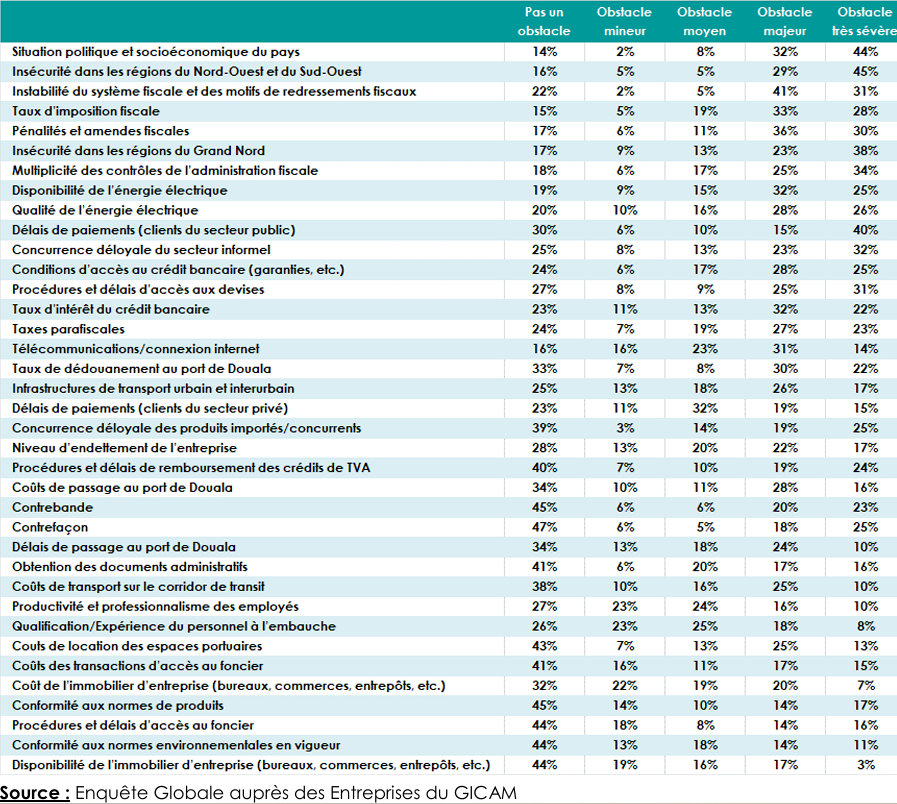
\includegraphics[width=0.8\textwidth]{enqueteGecam.png}
		\caption{récapitulatif de l'enquête du GECAM}
		\label{fig:mon_label}
	\end{figure}
	
	\subsubsection{Redaction du document de stratégie pour le developpement du secteur industriel par le MINEPAT}
	En 2022, le MINEPAT a engagé la rédaction d'un document de stratégie visant à proposer un nouveau cadre stratégique pour le secteur industriel, en réalignant la Stratégie de Développement du Secteur de l'Industrie et des Services (SDSIS) sur la planification post-Document Stratégique pour la Croissance Économique (DSCE). La démarche méthodologique adoptée s'est articulée en trois étapes: un état des lieux préalable de l'industrie camerounaise, une identification des problèmes susceptibles d'entraver le développement du secteur, et la proposition de stratégies assorties de mécanismes d'évaluation et de suivi. Les principaux résultats indiquent que la part de la valeur ajoutée manufacturière dans le PIB stagnait à 14,08\% en 2015, loin derrière des pays comparables tels que la Thaïlande (28,6\%) et la Malaisie (24\%); que 90\% des entreprises locales sont des très petites, petites ou moyennes entreprises; et que des projets structurants tels que le projet FABER et la construction de 8,000 km de voies ferrées ont été envisagés pour redynamiser le secteur \cite{minepat2022}. Les limites de ce document sont cependant notables: centré sur le seul secteur industriel, il n'évoque ni les besoins spécifiques des entreprises, ni les opportunités de partenariat inter-entreprises qui constituent pourtant un levier essentiel de compétitivité. \\
	
\subsubsection{Enquete sur le climat des affaires par le MINEPAT}
	Dans la continuité de ces travaux, le MINEPAT a lancé en novembre 2023 une enquête visant à préciser la manière dont les entreprises du secteur industriel perçoivent le climat des affaires, notamment en matière d'accès au financement, d'accès aux marchés et d'accès aux facteurs de production, ainsi que les actions menées par l'État en vue de l'améliorer. Sur le plan méthodologique, un échantillon de 1,000 entreprises a été constitué à l'échelle nationale en s'appuyant sur le réseau des délégués régionaux et départementaux du \gls{minepat}. Un questionnaire en ligne a été soumis, l'apurement et l'analyse des données collectées ont été effectués. Les résultats indiquent que 91\% des chefs d'entreprises considèrent que les coûts liés au taux d'intérêt, aux assurances et au courtage sont trop élevés, et appellent l'État à mettre en place des structures dédiées au financement des entreprises. L'accès aux facteurs de production et l'état des infrastructures routières sont unanimement identifiés comme des freins majeurs à la croissance. Malgré ces apports, l'étude reste circonscrite au seul secteur industriel et ne propose aucun mécanisme concret de mise en relation entre entreprises pour répondre aux besoins identifiés. \\
	
	\subsubsection{Recensement Général des Entreprises par l'INS}
	Enfin, le troisième Recensement Général des Entreprises (RGE3), réalisé par l'Institut National de la Statistique en 2023, avait pour objectifs d'actualiser le fichier des unités économiques nationales, de mettre en place un Système d'Information Géographique des entreprises et d'effectuer une analyse comparative avec les précédents recensements \cite{ins2023}. La méthodologie a consisté à constituer un fichier de base à partir des données administratives disponibles auprès de la Direction Générale des Impôts (DGI) et de la Caisse Nationale de Prévoyance Sociale (CNPS), puis à procéder à une collecte de terrain à l'aide d'outils numériques, après découpage du territoire national en douze Zones de Recensement \cite{ins2023}. Les résultats mettent en évidence une croissance significative du tissu entrepreneurial entre 2016 et 2023, avec une hausse de 109,5\% du nombre d'unités économiques, une prédominance du secteur tertiaire représentant 85,6\% des unités recensées, et une concentration très marquée des entreprises individuelles qui représentent 92,4\% du total. Cependant, en dépit de l'envergure de cet exercice, les défis rencontrés par les entreprises et leurs besoins spécifiques n'ont pas été documentés, et aucun outil de mise en relation entre acteurs économiques complémentaires n'a été envisagé à l'issue du recensement.\\
	
	\begin{figure}[H]           % H = ici exactement
		\centering
		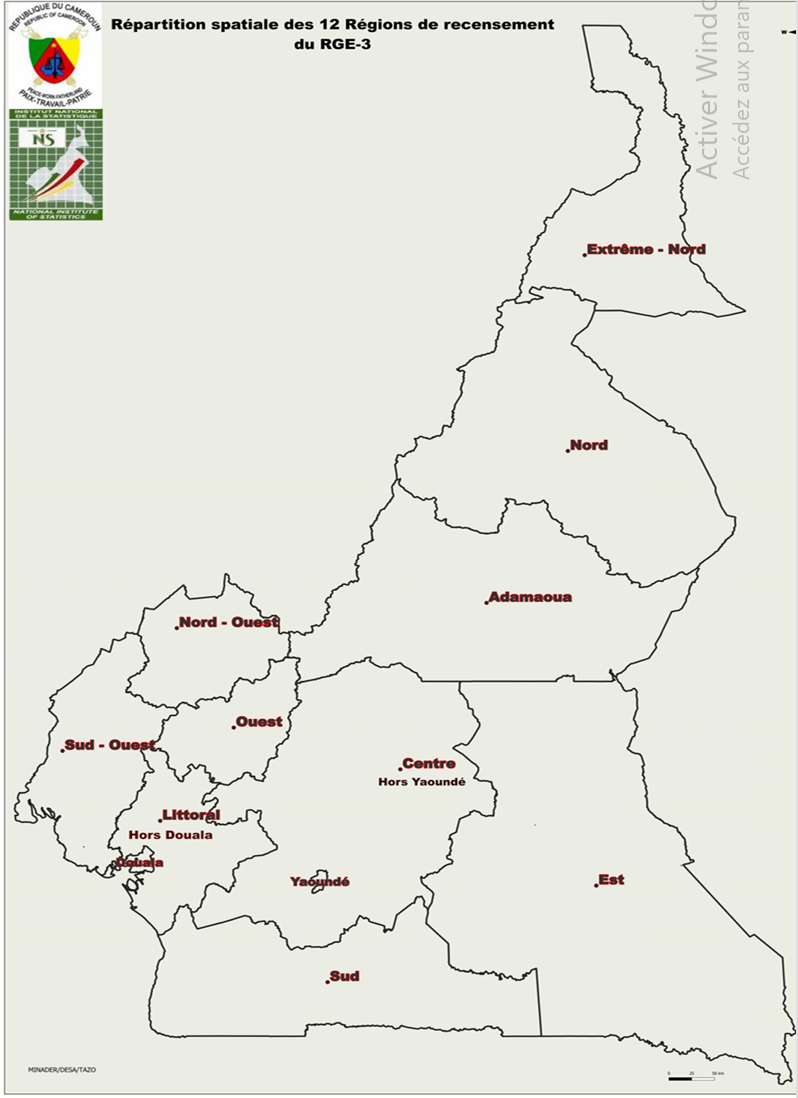
\includegraphics[width=0.8\textwidth]{zoneRecensement.png}
		\caption{Découpage des zones de recensement }
		\label{fig:zoneResencement}
	\end{figure}
	
\subsection{Plateformes existantes de mise en relation des entreprises}

Les plateformes numériques de mise en relation des entreprises se sont
considérablement multipliées au cours de la dernière décennie, portées
par la digitalisation croissante des échanges économiques et la montée
en puissance du commerce interentreprises en ligne. Chacune de ces
plateformes présente des caractéristiques, des fonctionnalités et des
positionnements distincts, répondant à des besoins variés selon les
secteurs d'activité, les zones géographiques et les types d'entreprises
ciblées. L'examen de ces plateformes existantes permet d'identifier les
bonnes pratiques à retenir, mais aussi les limites auxquelles la
plateforme gouvernementale développée dans le cadre de ce travail entend
apporter une réponse adaptée au contexte camerounais. Les principales
plateformes de mise en relation recensées dans la littérature et
utilisées à l'échelle internationale sont présentées ci-après.

\subsubsection{LinkedIn}

LinkedIn est largement reconnu comme le leader incontesté des réseaux
sociaux professionnels à l'échelle mondiale. Fondée en 2002 et rachetée
par Microsoft en 2016, la plateforme revendique aujourd'hui plus d'un
milliard d'utilisateurs répartis dans plus de 200 pays, ce qui en fait
l'écosystème numérique professionnel le plus étendu au monde \cite{linkedin2024}. LinkedIn
constitue un pilier incontournable dans l'univers du B2B en ce qu'il
offre aux entreprises un espace numérique dédié où elles peuvent établir
et soigner leur présence en ligne, se connecter avec d'autres acteurs
du marché et exploiter une multitude de fonctionnalités orientées vers
le développement commercial et le réseautage professionnel. Parmi ces
fonctionnalités, on peut notamment citer la création de pages entreprises
permettant de valoriser l'activité, les produits et les services proposés,
des outils de prospection ciblée permettant d'identifier des partenaires
potentiels selon des critères sectoriels, géographiques ou hiérarchiques,
ainsi que des espaces de publication de contenus favorisant la mise en
avant de l'expertise et le renforcement de la crédibilité de l'entreprise.
Cependant, malgré ses atouts indéniables, LinkedIn présente des limites
notables dans le contexte africain~:la
plateforme est principalement utilisée comme outil de réseautage
individuel et ne propose pas de mécanisme structuré de mise en relation
fondé sur les besoins spécifiques des entreprises.

\subsubsection{Facebook Marketplace}

Facebook Marketplace est une fonctionnalité intégrée à la plateforme
Facebook, lancée en 2016 par Meta, qui permet aux particuliers et aux
entreprises d'acheter, de vendre et d'échanger des biens et des services
au sein d'une communauté géographiquement délimitée. Avec plus de trois
milliards d'utilisateurs actifs sur Facebook à l'échelle mondiale,
Facebook Marketplace bénéficie d'une visibilité et d'une audience considérables,
ce qui en fait l'une des plateformes de commerce en ligne les plus
fréquentées au monde \cite{meta2024}. Dans le contexte africain et camerounais en
particulier, Facebook Marketplace présente un intérêt non négligeable~:
la forte pénétration de Facebook sur le continent, combinée à la
familiarité des utilisateurs avec l'interface de la plateforme, a conduit
de nombreuses petites entreprises et commerçants informels à y établir
une présence commerciale, parfois en l'absence de tout autre canal de
vente numérique. En ce sens, Facebook Marketplace a contribué à
l'émergence d'une forme de commerce numérique informel accessible à des
acteurs qui n'auraient pas eu les moyens de développer leur propre site
de vente en ligne.

Cependant, Facebook Marketplace présente plusieurs limites structurelles
qui en font un outil insuffisant pour répondre aux besoins de mise en
relation formelle entre entreprises dans le cadre d'une politique publique
d'appui au secteur privé. En premier lieu, la plateforme est principalement
conçue pour des échanges de proximité~: sa portée géographique est en
effet limitée à un rayon d'environ 65 kilomètres autour de la localisation
de l'utilisateur, ce qui rend impossible l'identification de partenaires
commerciaux situés dans d'autres régions du pays ou à l'étranger. En
deuxième lieu, Facebook Marketplace est un espace peu formalisé et
largement ouvert, ce qui le rend particulièrement vulnérable aux pratiques
frauduleuses, aux arnaques et aux transactions non sécurisées, nuisant
ainsi à la confiance des entreprises qui souhaiteraient y nouer des
partenariats sérieux et durables. En troisième lieu, la plateforme ne
dispose d'aucun mécanisme de vérification de l'identité ou de la
légitimité des vendeurs, ce qui limite considérablement la fiabilité des
informations qui y sont publiées. Ces limites rendent
cette plateforme inadaptée aux objectifs poursuivis par la plateforme
gouvernementale développée dans le cadre de ce travail.

\subsubsection{Alibaba}

Alibaba est une plateforme de commerce électronique B2B fondée en 1999
par Jack Ma en Chine, qui s'est imposée comme l'une des plus grandes
marketplaces mondiales dédiées aux échanges interentreprises. Elle met
en relation des fabricants, des grossistes, des fournisseurs et des
acheteurs professionnels issus de plus de 190 pays, couvrant des
secteurs aussi variés que l'industrie manufacturière, l'électronique,
le textile, l'agroalimentaire ou encore les équipements industriels.
Avec plusieurs dizaines de millions d'acheteurs actifs et des millions
de fournisseurs référencés, Alibaba constitue à ce jour l'une des
références mondiales en matière de mise en relation commerciale B2B
à l'échelle internationale\cite{alibaba2024}. La plateforme propose un ensemble de
fonctionnalités avancées permettant aux acheteurs de rechercher des
fournisseurs selon des critères précis tels que le pays d'origine,
le volume de production, la certification qualité ou encore la capacité
d'exportation, et aux fournisseurs de valoriser leurs capacités
productives auprès d'une audience internationale. Alibaba pallie ainsi
l'une des limites majeures de Facebook Marketplace en offrant une
portée véritablement mondiale, sans contrainte géographique.

Cependant, malgré ses atouts considérables, Alibaba présente des
limites importantes au regard des objectifs poursuivis dans le cadre
de ce travail. En premier lieu, la plateforme est essentiellement
orientée vers la vente de produits finis ou semi-finis en grande
quantité, ce qui la rend peu adaptée aux besoins des petites et
moyennes entreprises camerounaises qui recherchent des partenaires
locaux pour des collaborations de proximité, de la sous-traitance
ou du partage de ressources. En deuxième lieu, l'utilisation
d'Alibaba suppose une maîtrise suffisante de la langue anglaise
ou chinoise, ainsi qu'une capacité à gérer des transactions
internationales impliquant des procédures douanières, logistiques
et bancaires complexes, ce qui constitue un obstacle majeur pour
la majorité des entreprises du tissu productif camerounais. En
troisième lieu, la logique d'Alibaba est avant tout marchande et
transactionnelle~: la plateforme vise à conclure des ventes et non
à établir des partenariats stratégiques fondés sur une analyse des
besoins mutuels des entreprises. Elle ne propose donc aucun mécanisme
de recommandation basé sur la complémentarité des besoins et des
capacités, qui constitue pourtant le c\oe ur de la valeur ajoutée de
la plateforme développée dans ce travail. Enfin, les entreprises
camerounaises y sont quasi absentes en tant que fournisseurs référencés,
ce qui limite leur capacité à en tirer parti pour se faire connaître
à l'international.

	%============================================================
	%  CHAPITRE 3 : MÉTHODOLOGIE
	%============================================================
	%=============================================================
	\chapter{Cahier des charges de la plateforme
		\textit{Business Partnership}}
	\label{chap:cahier_charges}
	%=============================================================
	
	Le présent cahier des charges constitue le document de référence
	qui formalise l'ensemble des exigences fonctionnelles, techniques
	et non fonctionnelles auxquelles doit satisfaire la plateforme
	gouvernementale \textit{Business Partnership}. Il précise le
	contexte dans lequel s'inscrit le projet, les acteurs concernés,
	les cas d'usage attendus, les contraintes imposées et les critères
	de qualité retenus pour évaluer la solution livrée.
	
	%=============================================================
	\section{Périmètre du projet et identification des acteurs}
	\label{sec:contexte_projet}
	%=============================================================
	\subsection{Périmétre du projet}
	\subsubsection{Contexte institutionnel}
	
	La plateforme \textit{Business Partnership} s'inscrit dans le cadre
	de la mise en \oe uvre de la Stratégie Nationale de Développement
	2020--2030 (\gls{snd30}), qui identifie le développement du secteur
	privé comme l'un des leviers essentiels de la transformation
	structurelle de l'économie camerounaise. Elle constitue le
	prolongement numérique de l'enquête sur la cartographie et les
	besoins des entreprises conduite par le \gls{minepat} en 2025,
	dont les données collectées alimentent directement la base de
	connaissances de la plateforme et le moteur de mise en relation
	qui en constitue le c\oe ur fonctionnel. La plateforme est
	destinée à être opérée sous la tutelle du \gls{minepat}, qui
	en assurera la gouvernance et la maintenance, et à être accessible
	à l'ensemble des entreprises du tissu productif camerounais
	disposant d'un accès à internet.
	
	\subsubsection{Périmètre fonctionnel}
	
	Le périmètre de la plateforme \textit{Business Partnership} couvre
	les fonctionnalités suivantes~:
	
	\begin{itemize}
		\item la création et la gestion de comptes d'entreprises~;
		\item la saisie des besoins exprimés par
		les entreprises~;
		\item la mise en relation automatisée des entreprises sur la base
		d'un algorithme 
		\item l'administration et le suivi de la plateforme par les
		agents du \gls{minepat}.
	\end{itemize}
	
	
	%=============================================================
	%\section{Identification des acteurs}
	%\label{sec:acteurs}
	%=============================================================
	\subsection{Identifications des acteurs}
	L'identification précise des acteurs du système constitue un
	préalable indispensable à la définition des cas d'usage et à la
	modélisation des droits d'accès. Un acteur est défini ici comme
	toute entité --- humaine ou système externe --- qui interagit
	avec la plateforme \textit{Business Partnership} dans le cadre
	de son utilisation normale. Trois catégories d'acteurs principaux
	ont été identifiées.
	
	
	\subsubsection{L'entreprise (acteur principal)}
	
	L'entreprise constitue l'acteur central de la plateforme. Elle
	désigne toute unité économique --- quelle que soit sa taille,
	sa forme juridique ou son secteur d'activité --- qui s'inscrit
	sur la plateforme afin de renseigner son profil, d'exprimer
	ses besoins et de consulter les recommandations de partenaires
	potentiels générées par le moteur de mise en relation. L'entreprise
	est représentée sur la plateforme par un  utilisateur
	physique disposant d'un compte personnel sécurisé.
	
	\subsubsection{L'administrateur}
	
	L'administrateur est un agent du \gls{minepat} disposant de
	droits d'accès étendus à l'ensemble des fonctionnalités de la
	plateforme. Il est chargé de la validation des inscriptions des
	entreprises, du suivi
	des indicateurs d'utilisation et de l'administration technique
	de la plateforme. Il dispose d'un tableau de bord dédié lui
	permettant de superviser en temps réel l'ensemble des activités
	de la plateforme.
	
	\subsubsection{Le visiteur}
	
	Le visiteur désigne tout internaute qui accède à la plateforme
	sans être authentifié. Il peut consulter les informations
	publiques de présentation de la plateforme et ses fonctionnalités,
	mais ne peut accéder ni aux profils des entreprises, ni aux
	recommandations, ni à aucune fonctionnalité interactive. Son
	accès est strictement limité aux pages publiques, afin de
	protéger la confidentialité des informations des entreprises
	enregistrées.
	
	\begin{table}[H]
		\centering
		\caption{Synthèse des acteurs et de leurs droits d'accès}
		\label{tab:acteurs}
		\renewcommand{\arraystretch}{1.5}
		\begin{tabularx}{\textwidth}{>{\raggedright\arraybackslash}p{3cm}
				>{\centering\arraybackslash}p{2.2cm}
				>{\centering\arraybackslash}p{2.2cm}
				>{\centering\arraybackslash}X}
			\toprule
			\rowcolor{primary!15}
			\textbf{Fonctionnalité}
			& \textbf{Visiteur}
			& \textbf{Entreprise}
			& \textbf{Administrateur} \\
			\midrule
			
			\rowcolor{lightgray}
			Créer un compte entreprise
			& \textcolor{green!60!black}{\checkmark}
			& \textcolor{green!60!black}{\checkmark}
			& \textcolor{green!60!black}{\checkmark} \\
			
			Gérer son profil
			& \textcolor{accent}{\texttimes}
			& \textcolor{green!60!black}{\checkmark}
			& \textcolor{green!60!black}{\checkmark} \\
			
			\rowcolor{lightgray}
			Saisir ses besoins
			& \textcolor{accent}{\texttimes}
			& \textcolor{green!60!black}{\checkmark}
			& \textcolor{green!60!black}{\checkmark} \\
			
			Consulter les recommandations
			& \textcolor{accent}{\texttimes}
			& \textcolor{green!60!black}{\checkmark}
			& \textcolor{green!60!black}{\checkmark} \\
			
			\rowcolor{lightgray}
			Contacter un partenaire
			& \textcolor{accent}{\texttimes}
			& \textcolor{green!60!black}{\checkmark}
			& \textcolor{green!60!black}{\checkmark} \\
			
			\rowcolor{lightgray}
			Accéder au tableau de bord
			& \textcolor{accent}{\texttimes}
			& \textcolor{accent}{\texttimes}
			& \textcolor{green!60!black}{\checkmark} \\
			
			Gérer les utilisateurs
			& \textcolor{accent}{\texttimes}
			& \textcolor{accent}{\texttimes}
			& \textcolor{green!60!black}{\checkmark} \\
			
			\rowcolor{lightgray}
			Exporter les données
			& \textcolor{accent}{\texttimes}
			& \textcolor{accent}{\texttimes}
			& \textcolor{green!60!black}{\checkmark} \\
			
			\bottomrule
		\end{tabularx}
	\end{table}
	
	%=============================================================
	\section{Spécifications fonctionnelles et non fonctionnelles}
	\label{sec:specs_fonctionnelles}
	%=============================================================
	\subsection{Spécifications fonctionnelles}
	Les spécifications fonctionnelles décrivent de manière exhaustive
	et précise l'ensemble des fonctionnalités que doit offrir la
	plateforme \textit{Business Partnership} à ses différents acteurs.
	Chaque fonctionnalité est décrite sous la forme d'un cas d'usage
	(\textit{use case}), précisant les acteurs impliqués, les
	préconditions, le scénario nominal et les exceptions éventuelles.
	
	\subsubsection{Gestion des comptes et authentification}
	
	
		\textbf{Acteur principal~:} Représentant légal de l'entreprise \\
		\textbf{Préconditions~:} L'entreprise n'est pas encore enregistrée
		sur la plateforme \\
		\textbf{Scénario nominal~:}
		\begin{itemize}
			\item L'utilisateur accède au formulaire d'inscription depuis
			la page d'accueil de la plateforme~;
			\item Il renseigne les informations obligatoires~: raison sociale,
			statut juridique, région, secteur d'activité, adresse
			électronique et mot de passe~;
			\item Il soumet le formulaire~;
			\item Le système vérifie la validité et la cohérence des
			informations saisies~;
			\item L'administrateur valide l'inscription après vérification
			des informations~;
		\end{itemize}
		\textbf{Exceptions~:} Adresse électronique déjà utilisée~;
		informations incomplètes ou incohérentes.
	
	
	\vspace{0.5cm}
	
		\textbf{Acteur principal~:} Entreprise / Administrateur \\
		\textbf{Préconditions~:} L'utilisateur dispose d'un compte validé \\
		\textbf{Scénario nominal~:}
		\begin{itemize}
			\item L'utilisateur saisit son nom d'utilisateur et son
			mot de passe dans le formulaire de connexion~;
			\item Le système vérifie les identifiants~;
			\item En cas de succès, l'utilisateur est redirigé vers son
			tableau de bord personnel.
		\end{itemize}
		\textbf{Exceptions~:} Identifiants incorrects (maximum 5 tentatives
		avant verrouillage temporaire du compte)

	
	\subsubsection{Gestion des besoins}
	
		\textbf{Acteur principal~:} Entreprise \\
		\textbf{Préconditions~:} Le profil de l'entreprise est complété
		à au moins 50\,\% \\
		\textbf{Scénario nominal~:}
		\begin{enumerate}
			\item L'utilisateur accède à la secttion définir mes besoins automatiquement après l'enregistrement;
			\item Il sélectionne la catégorie de besoin parmi les types
			proposés (financement, équipements, intrants, transport,
			emballages, appui institutionnel, innovation)~;
			\item Il soumet le besoin~;
			\item Le système enregistre le besoin et déclenche la mise à
			jour des recommandations de partenaires.
		\end{enumerate}
		
	
	\subsubsection{Moteur de recommandation et mise en relation}
	

		\textbf{Acteur principal~:} Entreprise \\
		\textbf{Préconditions~:} Au moins un besoin a été saisi par
		l'entreprise \\
		\textbf{Scénario nominal~:}
		\begin{enumerate}
			\item L'utilisateur accède à la section \og{}Mes recommandations\fg{}~;
			\item Le système calcule la probabilité d'appartenance à chaque classe et retient la classe avec la plus grande probabilité;
			\item Il peut accéder au profil complet d'une entreprise
			recommandée.
		\end{enumerate}
	
\subsubsection{Administration de la plateforme}
	

	\textbf{Acteur principal :} Administrateur \par\smallskip
	\textbf{Préconditions :} L'administrateur est authentifié avec ses droits étendus \par\smallskip
	\textbf{Scénario nominal :}
	\begin{itemize}
		\item L'administrateur accède à son tableau de bord dédié ;
		\item Il consulte les indicateurs clés de la plateforme :
		nombre d'entreprises enregistrées, nombre de besoins
		saisis, nombre de mises en relation initiées;
		\item Il accède à la liste complète des entreprises et peut
		consulter, modifier ou suspendre tout profil.
	\end{itemize}

	%=============================================================
	%\section{Spécifications non fonctionnelles}
	%\label{sec:specs_non_fonctionnelles}
	%=============================================================
	\subsection{Spécifications non fonctionnelles}
	Les spécifications non fonctionnelles définissent les contraintes
	de qualité, de performance et de sécurité auxquelles la plateforme
	\textit{Business Partnership} doit se conformer, indépendamment
	des fonctionnalités qu'elle offre. Elles constituent des exigences
	transversales qui conditionnent la qualité globale de la solution
	et son adéquation aux contraintes du contexte camerounais.
	
	%\subsection{Exigences de performance}
	
	
	\subsubsection{Exigences de sécurité}
	
	La sécurité constitue une exigence fondamentale de la plateforme,
	en raison de la sensibilité des informations économiques et
	commerciales que les entreprises y déposent. Les mesures de
	sécurité suivantes sont imposées~:
	
	\begin{itemize}
		\item \textbf{Chiffrement des communications}~: l'ensemble des
		échanges entre le navigateur de l'utilisateur et le serveur de
		la plateforme doit être chiffré via le protocole
		\textbf{HTTPS/TLS}~;
		
		\item \textbf{Hachage des mots de passe}~: les mots de passe
		des utilisateurs doivent être stockés sous forme hachée à l'aide
		d'un algorithme cryptographiquement sûr (bcrypt ou Argon2),
		et ne doivent en aucun cas être stockés en clair dans la base
		de données~;
		
		\item \textbf{Protection contre les attaques courantes}~: la
		plateforme doit intégrer des mécanismes de protection contre
		les principales vulnérabilités web répertoriées par l'OWASP
		(\textit{Open Web Application Security Project}), notamment les
		injections SQL, les attaques par script intersite (XSS) et
		la falsification de requêtes intersites (CSRF). Le framework
		Django, retenu pour le développement, intègre nativement des
		mécanismes de protection contre ces attaques~;
		
		\item \textbf{Contrôle d'accès}~: un système de contrôle
		d'accès basé sur les rôles (\textit{Role-Based Access Control},
		RBAC) doit garantir qu'aucun utilisateur ne peut accéder à des
		ressources ou des fonctionnalités au-delà de celles autorisées
		par son profil~;
		
		\item \textbf{Journalisation des accès}~: les accès à la
		plateforme et les opérations sensibles (modification de profil,
		suppression de données, connexions administrateur) doivent
		être journalisés afin de permettre la traçabilité et l'audit.
	\end{itemize}
	
	\subsubsection{Exigences d'accessibilité et d'ergonomie}
	
	La plateforme doit être accessible depuis les navigateurs web
	modernes les plus répandus (Google Chrome, Mozilla Firefox,
	Microsoft Edge, Safari) dans leurs versions récentes, sans
	nécessiter l'installation de plugins ou d'extensions tierces.
	Elle doit adopter une conception \textit{responsive}, garantissant
	une expérience utilisateur satisfaisante aussi bien sur ordinateur
	de bureau que sur terminal mobile, ces derniers représentant le
	principal mode d'accès à internet pour une large fraction des
	utilisateurs camerounais. L'interface doit être rédigée intégralement
	en \textbf{langue française}, et son architecture de navigation
	doit respecter le principe de la règle des trois clics, selon
	lequel toute fonctionnalité doit être accessible depuis la page
	d'accueil en au plus trois interactions.
	
	\subsubsection{Exigences de maintenabilité et d'évolutivité}
	
	La plateforme doit être conçue selon les principes de l'architecture
	logicielle propre (\textit{clean architecture}), de manière à
	faciliter sa maintenance corrective et évolutive par des équipes
	techniques qui n'auraient pas participé à son développement initial.
	Le code source doit être intégralement documenté et versionné
	à l'aide du système Git, et déposé sur un dépôt accessible aux
	équipes techniques du \gls{minepat}. La base de données doit
	être conçue de manière modulaire, afin de permettre l'ajout de
	nouvelles variables d'analyse ou de nouvelles fonctionnalités
	sans nécessiter une refonte complète de l'architecture existante.
	

	%=============================================================
	\subsubsection{Diagramme des cas d'usage}
	\label{sec:use_case}
	%=============================================================
	
	Le diagramme des cas d'usage synthétise l'ensemble des interactions
	entre les acteurs identifiés et les fonctionnalités de la plateforme.
	Il constitue une représentation graphique standardisée, issue de la
	notation UML (\textit{Unified Modeling Language}), qui permet de
	communiquer de manière claire et non ambiguë les exigences
	fonctionnelles du système à l'ensemble des parties prenantes du
	projet, qu'elles soient techniques ou non \citep{booch_1998}.
	
	
	
	%=============================================================
	\subsubsection{Synthèse des exigences}
	\label{sec:synthese_exigences}
	%=============================================================
	
	Le tableau~\ref{tab:synthese_exigences} ci-dessous présente une
	synthèse récapitulative de l'ensemble des exigences du cahier des
	charges, organisées par catégorie et accompagnées de leur niveau
	de priorité selon la méthode \textbf{MoSCoW}
	(\textit{Must have, Should have, Could have, Won't have}),
	qui constitue l'une des techniques de priorisation des exigences
	les plus répandues dans les projets agiles \citep{anderson2015essential}.
\begin{table}[H]
	\centering
	\caption{Synthèse des exigences selon la méthode MoSCoW}
	\label{tab:synthese_exigences}
	\renewcommand{\arraystretch}{1.4}
	\begin{tabularx}{\textwidth}{>{\raggedright\arraybackslash}p{1.5cm}
			>{\raggedright\arraybackslash}X
			>{\centering\arraybackslash}p{2.5cm}}
		\toprule
		\rowcolor{primary!15}
		\textbf{Catégorie} & \textbf{Exigence} & \textbf{Priorité MoSCoW} \\
		\midrule
		
		\multirow{10}{1.5cm}{\raggedright\textbf{Fonction-\\nel}}
		& Inscription et authentification des entreprises
		& \textbf{Must have} \\
		& Gestion du profil d'entreprise
		& \textbf{Must have} \\
		\rowcolor{lightgray}
		& Saisie et gestion des besoins
		& \textbf{Must have} \\
		& Moteur de recommandation (similarité cosinus)
		& \textbf{Must have} \\
		\rowcolor{lightgray}
		& Messagerie interne entre entreprises
		& \textbf{Should have} \\
		& Cartographie géographique interactive
		& \textbf{Should have} \\
		\rowcolor{lightgray}
		& Tableau de bord administrateur
		& \textbf{Must have} \\
		& Export des données (CSV)
		& \textbf{Should have} \\
		\rowcolor{lightgray}
		& Système de notation des partenariats
		& \textbf{Could have} \\
		& Intégration avec les SI des administrations
		& \textbf{Won't have} \\
		
		\midrule
		
		\multirow{5}{1.5cm}{\raggedright\textbf{Non\\fonction-\\nel}}
		& Temps de réponse $\leq$ 3 secondes
		& \textbf{Must have} \\
		\rowcolor{lightgray}
		& Chiffrement HTTPS/TLS
		& \textbf{Must have} \\
		& Interface \textit{responsive} (mobile)
		& \textbf{Must have} \\
		\rowcolor{lightgray}
		& Disponibilité $\geq$ 99\,\%
		& \textbf{Should have} \\
		& Support multilingue (français/anglais)
		& \textbf{Could have} \\
		
		\bottomrule
	\end{tabularx}
\end{table}
	Ce cahier des charges constitue le document contractuel de référence
	sur lequel s'est fondé l'ensemble du processus de conception et de
	développement de la plateforme \textit{Business Partnership}. Les
	exigences classées \textit{Must have} ont été intégralement
	implémentées dans la version présentée dans ce mémoire. Les exigences
	\textit{Should have} ont été partiellement développées et constituent
	des axes prioritaires d'évolution pour les versions ultérieures.
	Les exigences \textit{Could have} et \textit{Won't have} ont été
	documentées et transmises aux équipes techniques du \gls{minepat}
	comme feuille de route pour les développements futurs de la plateforme.
	
	
	\chapter{Conception, modélisation et implémentation}
	Il sera question dans ce chapitre de présenter la méthodologie utilisée en vue du traitement des données issues de  l’enquête réalisée par le MINEPAT sur la cartographie des besoins des entreprises. Nous débuterons par une présentation des données à travers la description de la source des données, des variables et en fin les méthodes de traitements de ces données. S’en suivra la méthodologie sur la conception de la plateforme gouvernementale et des techniques utilisées.
	\label{chap:methodo}
	
	\section{Méthodologie pour la cartographie des besoins des entreprises}
	
	\subsection{Présentation des données}
	\subsubsection{Source de données}
	L’enquête réalisée par le MINEPAT s’est fait à travers la soumission d’un formulaire électronique par les entreprises cibles. De cette soumission une base de données a pu être constituée résultat des réponses des entreprises qui faisaient l’objet de l’enquête. Le traitement de ces données s’est effectué dans le strict respect des procédures et outils statistiques. Le fichier identifications.csv regroupe l'ensemble des informations permettant d'identifier et de caractériser les entreprises enquêtées. Il contient des variables relatives à la dénomination de l'entreprise, à sa localisation géographique, à son secteur d'activité, à sa forme juridique, à son année de création et à sa taille. Ce fichier constitue la dimension cartographique de la base de données, en ce qu'il permet de positionner chaque entreprise dans le tissu économique national selon plusieurs axes d'analyse. Le fichier besoins.csv, quant à lui, recense les besoins exprimés par les entreprises en réponse aux questions posées dans le formulaire. Il contient des informations sur les types de besoins identifiés par les entreprises qu'ils soient d'ordre financier, organisationnel, technologique ou commercial. Ce fichier constitue la dimension analytique de la base de données, sur laquelle repose la logique de recommandation de la plateforme.  Ces deux fichiers ont été joints par un identifiant unique attribué à chaque entreprise lors de la collecte, permettant d'associer à chaque unité économique ses caractéristiques d'identification et ses besoins exprimés. Avant toute analyse, une phase d'apurement des données a été réalisée afin de traiter les valeurs manquantes, d'identifier les doublons éventuels et de vérifier la cohérence des réponses fournies.
	\subsubsection{Description des variables}
	Les variables utilisées lors de cette enquête sont essentiellement qualitative et sont orientées dans deux buts principaux : identifier de la manière la plus précise les entreprises et obtenir des informations les plus complètes sur leurs besoins. Nous nous proposons de décrire ces variables dans les tableaux qui suivent.
	
	%------------------------------------------------------------------
	% Tableau 1 : Variables d'identification
	%------------------------------------------------------------------
	\begin{table}[H]
		\centering
		\caption{Variables pour l'identification des entreprises
			(\texttt{identifications.csv})}
		\label{tab:var_identification}
		\renewcommand{\arraystretch}{1.5}
		\begin{tabularx}{\textwidth}{
				>{\ttfamily\raggedright\arraybackslash}p{3.8cm}
				>{\raggedright\arraybackslash}p{2.8cm}
				>{\raggedright\arraybackslash}X}
			
			\toprule
			\rowcolor{primary!15}
			\textbf{Variable} & \textbf{Type} & \textbf{Commentaire} \\
			\midrule
			
			id
			& Qualitatif nominal
			& Entier attribué automatiquement par la plateforme en fonction
			de la date de soumission du formulaire. \\
			
			\rowcolor{lightgray}
			raison\_sociale
			& Qualitatif nominal
			& Permet d'obtenir la dénomination sous laquelle l'entreprise
			s'est enregistrée. \\
			
			statut\_juridique
			& Qualitatif nominal
			& Permet d'obtenir le statut juridique de l'entreprise
			(SARL, SA, EI, etc.). \\
			
			\rowcolor{lightgray}
			autre\_statut\_juridique
			& Qualitatif nominal
			& Champ de saisie libre permettant à l'entreprise d'indiquer
			son statut juridique lorsque celui-ci ne figure pas parmi
			les modalités proposées dans le formulaire. \\
			
			region
			& Qualitatif nominal
			& Permet d'identifier la région dans laquelle évolue
			l'entreprise parmi les dix régions du Cameroun. \\
			
			\rowcolor{lightgray}
			localisation
			& Qualitatif nominal
			& Permet d'obtenir des informations plus précises sur
			l'emplacement de l'entreprise, au niveau du quartier
			ou de la ville. \\
			
			taille\_entreprise
			& Qualitatif nominal
			& Fait référence aux différentes catégories d'entreprises
			rencontrées au Cameroun selon leur taille
			(TPE, PE, PME, GE). \\
			
			\rowcolor{lightgray}
			date\_debut\_activite
			& Qualitatif nominal
			& Renvoie à la date effective de démarrage des activités
			de l'entreprise. \\
			
			secteur\_activite
			& Qualitatif ordinal
			& Fait référence au secteur d'activité auquel appartient
			l'entreprise (primaire, secondaire ou tertiaire). \\
			
			\rowcolor{lightgray}
			secteur\_autre
			& Qualitatif ordinal
			& Champ de saisie libre permettant d'enregistrer un secteur
			d'activité autre que ceux proposés dans le formulaire. \\
			
			branche\_activite
			& Qualitatif nominal
			& Permet d'identifier la branche d'activité dans laquelle
			évolue l'entreprise au sein de son secteur. \\
			
			\rowcolor{lightgray}
			branche\_autre
			& Qualitatif nominal
			& Champ de saisie libre permettant d'enregistrer une branche
			d'activité autre que celles proposées dans le formulaire. \\
			
			bien\_services
			& Qualitatif nominal
			& Permet d'identifier les biens et services proposés
			par l'entreprise à sa clientèle. \\
			
			\rowcolor{lightgray}
			telephone
			& Qualitatif nominal
			& Adresse téléphonique de l'entreprise permettant
			de la contacter. \\
			
			email
			& Qualitatif nominal
			& Adresse électronique de l'entreprise. \\
			
			\rowcolor{lightgray}
			site\_web
			& Qualitatif nominal
			& URL du site web de l'entreprise, le cas échéant. \\
			
			date\_soumission
			& Qualitatif nominal
			& Date à laquelle l'entreprise a soumis le formulaire
			sur la plateforme de collecte. \\
			
			\bottomrule
		\end{tabularx}
	\end{table}
	
	%------------------------------------------------------------------
	% Tableau 2 : Variables des besoins
	%------------------------------------------------------------------
	\begin{table}[H]
		\centering
		\caption{Variables relatives aux besoins des entreprises
			(\texttt{besoins.csv})}
		\label{tab:var_besoins}
		\renewcommand{\arraystretch}{1.5}
		\begin{tabularx}{\textwidth}{
				>{\ttfamily\raggedright\arraybackslash}p{3.8cm}
				>{\raggedright\arraybackslash}p{2.8cm}
				>{\raggedright\arraybackslash}X}
			
			\toprule
			\rowcolor{primary!15}
			\textbf{Variable} & \textbf{Type} & \textbf{Commentaire} \\
			\midrule
			
			entreprise\_id
			& Qualitatif nominal
			& Clé étrangère faisant référence à l'identifiant unique
			(\texttt{id}) de l'entreprise dans le fichier
			\texttt{identifications.csv}. Permet d'associer chaque
			besoin à l'entreprise correspondante. \\
			
			\rowcolor{lightgray}
			type\_besoin
			& Qualitatif nominal
			& Fait référence à la catégorie de besoin exprimé par
			l'entreprise (besoin financier, technologique,
			commercial, organisationnel, etc.). \\
			
			detail\_besoin
			& Qualitatif nominal
			& Permet de décrire avec plus de précision la nature
			du besoin exprimé, en complément de la catégorie
			renseignée dans la variable \texttt{type\_besoin}. \\
			
			\rowcolor{lightgray}
			plateforme\_existante
			& Qualitatif nominal
			& Fait référence aux moyens ou plateformes de mise en
			relation auxquels l'entreprise a déjà souscrit ou
			qu'elle utilise actuellement pour trouver des
			partenaires commerciaux. \\
			
			\bottomrule
		\end{tabularx}
	\end{table}
	\subsubsection{Pré-traitement de la Base de Données}
	
	Avant toute analyse statistique, il est recommandé d'effectuer une phase de prétraitement des données afin d'en garantir la qualité et la cohérence. Cette étape, souvent désignée sous le terme de data cleaning dans la littérature en Data Sciences, constitue un préalable indispensable à la fiabilité des résultats. Elle a comporté les opérations suivantes:
	
	\begin{itemize}
		\item \textbf{Organisation des données} :
		
		
		La première étape du traitement a consisté à rendre stable la structure de la base de données afin de disposer d’un fichier exploitable pour l’analyse. La base initiale comportait une table principale décrivant le profil des entreprises et une table secondaire renseignant les besoins exprimés. Comme une même entreprise pouvait déclarer plusieurs besoins, la table des besoins contenait plusieurs lignes pour une seule entreprise. Il n’était donc pas pertinent de faire une simple jointure ligne à ligne, car cela aurait multiplié artificiellement certaines entreprises dans la base finale. Le traitement a plutôt consisté à ramener les besoins au niveau de l’entreprise, de manière à conserver une seule ligne par entreprise dans la table principale, tout en ajoutant les informations relatives aux besoins sous forme de variables distinctes.\\
		
		\item \textbf{Transformation des données}
		
		La deuxième étape a porté sur la transformation de la table des besoins en variables binaires de type Oui/Non. Chaque type de besoin initialement déclaré dans la feuille des besoins a été converti en une colonne spécifique. Lorsqu’une entreprise avait déclaré un besoin donné, la modalité « Oui » lui était attribuée ; dans le cas contraire, la modalité « Non » était retenue. Cette opération permet de rendre les besoins directement comparables entre entreprises, tout en évitant les problèmes liés au format long de la table initiale. Elle facilite aussi l’exploitation statistique, car chaque entreprise est décrite à la fois par ses caractéristiques propres et par l’ensemble des besoins qu’elle a ou n’a pas exprimés.\\
		
		\item \textbf{Discrétisation des données} :
		La troisième étape a consisté à harmoniser certaines informations mal structurées ou hétérogènes, notamment la variable relative à la date de début d’activité. Cette variable contenait des formats variés : années simples, dates complètes, valeurs numériques issues d’Excel, textes partiels ou informations difficilement exploitables. Pour rendre cette information utilisable, elle a été transformée en classes d’âge de l’entreprise : « Moins de 3 ans », « 3 à 4 ans », « 5 à 9 ans », « 10 à 19 ans », « 20 ans et plus » et « Non renseigné ». Ce choix permet de passer d’une information brute parfois instable à une variable catégorielle claire, homogène et interprétable. Il permet également de comparer les entreprises selon leur niveau de maturité, ce qui est plus pertinent qu’une date brute souvent mal renseignée.\\
		
		\item \textbf{Supression des données}:
		
		
		La quatrième étape a concerné la rationalisation des besoins exprimés. Certains besoins étaient très proches sur le fond, mais apparaissaient sous des libellés séparés. C’est le cas, par exemple, des besoins liés aux équipements de conditionnement, de conservation ou de stockage, de production et de transformation. Ces différentes modalités ont été regroupées dans une seule variable appelée besoin\_equipements, car elles renvoient toutes à une contrainte matérielle ou productive. De la même manière, les besoins relatifs aux nouvelles techniques de conditionnement, de conservation ou stockage, de production et de transformation ont été regroupés dans une variable appelée besoin\_innovation\_recherche, qui traduit davantage un besoin d’innovation, d’amélioration technique ou d’accompagnement en recherche appliquée. Cette consolidation permet de réduire la dispersion des modalités et de rendre les résultats plus lisibles.\\
		
		\item 
		Enfin, la dernière étape a consisté à uniformiser les modalités textuelles et à produire une base finale cohérente, prête pour l’analyse statistique. Les accents ont été retirés sur les modalités afin d’éviter que deux valeurs identiques sur le fond soient traitées comme différentes à cause de variations d’écriture. Les besoins ont été regroupés en sept grandes catégories finales, ce qui permet de conserver l’essentiel de l’information tout en simplifiant la lecture économique des résultats. Au terme du traitement, chaque entreprise est décrite par son profil et par un ensemble réduit, clair et homogène de besoins. Cette structuration est particulièrement pertinente, car elle permet de comparer les entreprises entre elles et de repérer plus facilement les proximités entre profils d’entreprises et types de besoins exprimés.
	\end{itemize}
	\subsection{Méthode d'analyse}
	Le traitement de la base de données passe par l’utilisation d’un ensemble de méthodes, les objectifs ici sont la description et l’exploration du jeu de données à disposition. 
	\subsubsection{Analyse descriptive}
	L’analyse descriptive constitue la première étape d’exploitation statistique de la base. Elle permet de comprendre la structure générale des entreprises enquêtées avant tout regroupement plus avancé. Cette étape repose sur deux niveaux complémentaires : l’analyse univariée, qui décrit chaque variable séparément, et l’analyse bivariée, qui met en relation les caractéristiques des entreprises avec les besoins exprimés. Cette progression est importante, car elle évite d’interpréter directement des groupes complexes sans avoir d’abord identifié les principales tendances de la base.
	\begin{enumerate}
		\item \textbf{Analyse uni-variée}:
		
		L’analyse univariée vise d’abord à présenter la distribution des entreprises selon leurs principales caractéristiques : statut juridique, région, taille, ancienneté et secteur d’activité principal. Pour chaque variable, les effectifs et les pourcentages sont calculés afin de connaître le poids de chaque modalité dans l’ensemble de la base. La logique est la suivante : une modalité fortement représentée peut influencer les résultats globaux, tandis qu’une modalité faiblement représentée doit être interprétée avec prudence. Par exemple, si une région ou un secteur concentre une grande partie des entreprises, les besoins observés au niveau global peuvent en partie refléter cette concentration.\\
		
		Les besoins exprimés par les entreprises sont également analysés de manière univariée. L’objectif est d’identifier les besoins les plus fréquents parmi les sept catégories retenues : intrants, financement, emballages, transport, appui à l’entreprise, équipements, innovation et recherche. Pour chaque besoin, l’analyse consiste à compter le nombre d’entreprises ayant répondu « Oui », puis à rapporter cet effectif au nombre total d’entreprises. Le pourcentage obtenu indique la proportion d’entreprises concernées par chaque besoin. Cette étape permet de hiérarchiser les contraintes exprimées et de distinguer les besoins transversaux, qui touchent une grande partie des entreprises, des besoins plus spécifiques.\\
		
		
	\item \textbf{Analyse bis-variée}:
	
L’analyse bivariée intervient ensuite pour dépasser la simple description globale. Elle consiste à croiser les variables de profil avec les variables de besoins afin de déterminer si certains types d’entreprises expriment davantage certains besoins. Par exemple, les besoins de financement peuvent être croisés avec la taille des entreprises, les besoins en équipements avec le secteur d’activité, ou encore les besoins d’appui avec l’ancienneté. Cette étape permet de répondre à une question centrale : les besoins sont-ils répartis de manière uniforme entre toutes les entreprises, ou varient-ils selon leur profil ?\\

L’intérêt de l’analyse bivariée est donc de produire une lecture plus ciblée des besoins. Une analyse globale peut montrer qu’un besoin est important, mais elle ne dit pas nécessairement quels types d’entreprises sont les plus concernés. Le croisement des variables permet de préciser cette information. Par exemple, si les petites entreprises déclarent plus fréquemment un besoin de financement, cela suggère que la contrainte financière est particulièrement associée à leur profil. Si les entreprises d’un secteur donné déclarent davantage des besoins en équipements, cela peut révéler une contrainte productive ou technologique propre à ce secteur.\\

Pour renforcer l’interprétation des croisements, le test du $\chi^2$ est mobilisé. Ce test permet de vérifier si la relation observée entre une variable de profil et un besoin est statistiquement significative. L’hypothèse testée est l’indépendance entre les deux variables. Lorsque la p-value est inférieure à 5 \%, l’hypothèse d’indépendance est rejetée : il existe alors une association statistique entre la caractéristique de l’entreprise et le besoin considéré. À l’inverse, lorsque la p-value est supérieure à 5 \%, la relation observée n’est pas suffisamment robuste pour être considérée comme significative.\\

Lorsque le test du $\chi^2$ indique une association significative, l’intensité de cette association peut être appréciée à l’aide du V de Cramer. Cette mesure permet de distinguer une relation faible, modérée ou forte. Elle est utile parce qu’une association peut être statistiquement significative tout en étant peu importante sur le plan pratique. Le V de Cramer complète donc le Khi-deux en indiquant non seulement si deux variables sont liées, mais aussi à quel degré elles le sont. Dans l’analyse, cette étape permet de retenir les associations réellement pertinentes pour comprendre la structuration des besoins des entreprises.
	\end{enumerate}

	\subsubsection{Analyse exploratoire des données}
	Après les analyses univariée et bivariée, l’analyse multivariée permet d’étudier simultanément l’ensemble des variables de profil et des besoins. Cette étape est nécessaire, car les entreprises ne se différencient pas seulement par une variable isolée. Elles se distinguent plutôt par une combinaison de caractéristiques : taille, secteur, ancienneté, région, statut juridique et besoins exprimés. Les méthodes multivariées permettent donc de passer d’une lecture variable par variable à une lecture globale des profils d’entreprises. Dans cette logique, l’Analyse des Correspondances Multiples (ACM), la Classification Ascendante Hiérarchique (CAH) puis l'Anayse Factorielle Discrimimante (AFD) sont mobilisées.
	\begin{enumerate}
		\item \textbf{Analyse en Composante Multiple}:
		
		\paragraph{Notion d'ACM}
	L’Analyse des Correspondances Multiples est adaptée aux données qualitatives. Elle permet de résumer l’information contenue dans plusieurs variables catégorielles et de représenter les entreprises et les modalités dans un espace factoriel commun. Son intérêt est particulièrement fort dans cette étude, car les variables utilisées sont essentiellement qualitatives : les caractéristiques des entreprises sont exprimées sous forme de catégories, et les besoins sont codés en modalités « Oui » ou « Non ». L’ACM permet ainsi d’identifier les proximités entre modalités et de voir quelles caractéristiques tendent à apparaître ensemble.\\
	
	L’interprétation de l’ACM repose d’abord sur les axes factoriels. Chaque axe résume une partie des différences entre les entreprises. Les valeurs propres indiquent la part d’information portée par chaque dimension. En ACM, les pourcentages d’inertie sont souvent relativement faibles, surtout lorsque plusieurs variables qualitatives sont utilisées. Cela n’invalide pas l’analyse. L’essentiel est d’identifier les modalités qui contribuent le plus à chaque axe, car ce sont elles qui donnent un sens économique aux dimensions retenues. Les axes ne sont donc pas interprétés uniquement à partir de leur inertie, mais surtout à partir des modalités qui les structurent.\\
	
	Les contributions des modalités permettent de repérer les catégories qui jouent le rôle le plus important dans la construction des axes. Une modalité fortement contributive participe fortement à la différenciation des entreprises. Le cosinus carré complète cette information en indiquant si la modalité est bien représentée sur l’axe considéré. Une modalité à la fois fortement contributive et bien représentée est particulièrement utile pour interpréter l’axe. À l’inverse, une modalité très rare ou faiblement représentée doit être commentée avec prudence, même lorsqu’elle apparaît visible sur la carte factorielle.\\
	
	Les cartes factorielles issues de l’ACM facilitent la lecture des relations entre profils et besoins. Sur la carte des modalités, deux modalités proches peuvent être interprétées comme associées. Par exemple, la proximité entre une catégorie de taille d’entreprise et un besoin donné peut suggérer que ce besoin est plus fréquent pour cette catégorie. Les modalités éloignées du centre sont celles qui différencient le plus les entreprises, tandis que les modalités proches du centre sont moins discriminantes. Sur la carte des individus, chaque point représente une entreprise ; les entreprises proches les unes des autres présentent des profils relativement similaires.
		\paragraph{Formalisation mathématique}
		Soit un tableau de données $X$ composé de $n$ individus (entreprises)
		décrits par $p$ variables qualitatives $Q_1, Q_2, \ldots, Q_p$, où la
		variable $Q_j$ admet $m_j$ modalités. Le nombre total de modalités est
		noté $m = \sum_{j=1}^{p} m_j$. L'ACM repose sur la transformation de
		ce tableau en un \textbf{tableau disjonctif complet} (TDC) $Z$ de
		dimension $n \times m$, dans lequel chaque variable qualitative $Q_j$
		est recodée en $m_j$ variables binaires~:
		
		\begin{equation}
			z_{ik}^{(j)} =
			\begin{cases}
				1 & \text{si l'individu } i \text{ présente la modalité } k
				\text{ de la variable } Q_j \\
				0 & \text{sinon}
			\end{cases}
			\label{eq:tdc}
		\end{equation}
	Le tableau de Burt $\mathbf{B}$ est défini comme le produit :
	
	\begin{equation}
		\mathbf{B} = \mathbf{Z}^{\top} \mathbf{Z} \in \mathbb{R}^{K \times K}.
		\label{eq:burt}
	\end{equation}
	
	Il regroupe en sous-blocs les tableaux de contingence croisés entre toutes les paires
	de variables, et les tableaux diagonaux contenant les effectifs marginaux de chaque
	modalité.
	
	On définit les matrices diagonales de pondération :
	
	\begin{equation}
		\mathbf{D}_r = \frac{1}{nQ}\,\mathbf{Z}^{\top}\mathbf{1}_n, \qquad
		\mathbf{D}_c = \frac{1}{nQ}\,\mathbf{Z}^{\top}\mathbf{1}_n,
	\end{equation}
	
	où $\mathbf{1}_n$ est le vecteur unité de taille $n$. La matrice des profils ligne
	(profils des individus sur les modalités) est :
	
	\begin{equation}
		\mathbf{P} = \frac{1}{nQ}\,\mathbf{Z}.
		\label{eq:profils}
	\end{equation}
	
	La matrice à décomposer est alors la matrice des écarts à l'indépendance :
	
	\begin{equation}
		\mathbf{S} = \mathbf{D}_r^{-1/2}
		\left(\mathbf{P} - \mathbf{r}\,\mathbf{c}^{\top}\right)
		\mathbf{D}_c^{-1/2},
		\label{eq:ecarts}
	\end{equation}
	
	où $\mathbf{r} = \mathbf{P}\,\mathbf{1}_K$ et $\mathbf{c} = \mathbf{P}^{\top}\mathbf{1}_n$
	sont respectivement les marges lignes et colonnes de $\mathbf{P}$.
	
	% --- 1.4 Décomposition en valeurs singulières et vecteurs propres ---
	
	
	L'ACM repose sur la Décomposition en Valeurs Singulières (DVS) de la matrice
	$\mathbf{S}$ définie en~\eqref{eq:ecarts} :
	
	\begin{equation}
		\mathbf{S} = \mathbf{U}\,\boldsymbol{\Sigma}\,\mathbf{V}^{\top},
		\label{eq:svd}
	\end{equation}
	
	où :
	\begin{itemize}
		\item $\mathbf{U} \in \mathbb{R}^{n \times r}$ contient les vecteurs singuliers
		gauches (vecteurs propres des individus) ;
		\item $\mathbf{V} \in \mathbb{R}^{K \times r}$ contient les vecteurs singuliers
		droits (vecteurs propres des modalités) ;
		\item $\boldsymbol{\Sigma} = \mathrm{diag}(\sigma_1, \sigma_2, \ldots, \sigma_r)$
		est la matrice diagonale des valeurs singulières, avec
		$\sigma_1 \geq \sigma_2 \geq \cdots \geq \sigma_r \geq 0$.
	\end{itemize}
	
	Les valeurs propres associées à chaque axe factoriel sont :
	
	\begin{equation}
		\lambda_s = \sigma_s^2, \quad s = 1, \ldots, r.
		\label{eq:valeurs_propres}
	\end{equation}
	
	Les vecteurs propres $\mathbf{v}_s$ (colonnes de $\mathbf{V}$) sont solutions du
	problème aux valeurs propres :
	
	\begin{equation}
		\mathbf{S}^{\top}\mathbf{S}\,\mathbf{v}_s = \lambda_s\,\mathbf{v}_s,
		\qquad \|\mathbf{v}_s\| = 1.
		\label{eq:vp_modalites}
	\end{equation}
	
	La part de variance totale expliquée par l'axe $s$ est mesurée par le taux d'inertie :
	
	\begin{equation}
		\tau_s = \frac{\lambda_s}{\displaystyle\sum_{s'=1}^{r} \lambda_{s'}}.
		\label{eq:inertie}
	\end{equation}
	
	% --- 1.5 Projection dans le nouvel espace factoriel ---
	
	
	Une fois les vecteurs propres obtenus, les coordonnées factorielles des individus
	sur les axes de l'ACM sont calculées par projection dans le nouvel espace. Les
	coordonnées de l'individu $i$ sur l'axe $s$ sont données par :
	
	\begin{equation}
		F_{is} = \frac{1}{\sigma_s}\,\sum_{k=1}^{K} p_{ik}\,v_{ks},
		\label{eq:coord_individus}
	\end{equation}
	
	où $p_{ik}$ est l'élément $(i,k)$ de $\mathbf{P}$ et $v_{ks}$ est la $k$-ième
	composante du $s$-ième vecteur propre. En notation matricielle :
	
	\begin{equation}
		\boxed{\mathbf{F} = \mathbf{D}_r^{-1/2}\,\mathbf{U}\,\boldsymbol{\Sigma}}
		\label{eq:proj_individus}
	\end{equation}
	
	De même, les coordonnées des modalités sur l'axe $s$ sont :
	
	\begin{equation}
		G_{ks} = \frac{1}{\sigma_s}\,\sum_{i=1}^{n} p_{ik}\,u_{is},
		\label{eq:coord_modalites}
	\end{equation}
	
	soit en notation matricielle :
	
	\begin{equation}
		\boxed{\mathbf{G} = \mathbf{D}_c^{-1/2}\,\mathbf{V}\,\boldsymbol{\Sigma}}
		\label{eq:proj_modalites}
	\end{equation}
	
	Les matrices $\mathbf{F}$ et $\mathbf{G}$ constituent le nouvel espace factoriel
	dans lequel individus et modalités sont représentés simultanément, ce qui est la
	propriété centrale du biplot en ACM.
	\item Classification Ascendante Hiérarchique (CAH):
	
	\paragraph{Notion de CAH}
	La Classification Ascendante Hiérarchique est ensuite réalisée à partir des coordonnées factorielles de l’ACM. Cette articulation est méthodologiquement pertinente, car la classification ne s’appuie pas directement sur les variables brutes, mais sur une représentation synthétique des principales différences entre entreprises. L’ACM réduit la complexité de l’information, puis la CAH utilise cette information pour constituer des groupes homogènes. Le principe est de regrouper progressivement les entreprises les plus proches jusqu’à obtenir une partition finale. Dans le cas retenu, la classification est contrainte à trois classes afin d’obtenir une typologie lisible et opérationnelle.\\
	
	Le choix de trois classes répond à une logique de synthèse. Un nombre trop élevé de classes rendrait l’interprétation plus complexe et risquerait de produire des groupes trop fragmentés pour l’aide à la décision. À l’inverse, un nombre trop faible pourrait masquer des différences importantes entre entreprises. Trois classes permettent de dégager une typologie équilibrée, suffisamment simple pour être exploitable, mais assez différenciée pour mettre en évidence plusieurs profils de besoins. Chaque classe regroupe donc des entreprises relativement proches en termes de caractéristiques et de besoins exprimés.\\
	
	L’interprétation finale repose sur le profilage des classes. Une fois les groupes constitués, chaque classe est décrite selon la taille des entreprises, la région, le secteur d’activité, l’ancienneté et les besoins déclarés. Cette étape est essentielle, car la CAH fournit des groupes statistiques, mais leur sens économique doit être construit à partir des modalités qui les caractérisent. Les tableaux de profilage permettent d’identifier les caractéristiques dominantes de chaque groupe. Le taux de déclaration des besoins par classe est particulièrement important, car il permet de nommer les classes selon leur contenu réel : classe à dominante productive, financière, logistique, organisationnelle ou orientée vers l’innovation.\\
	
	
	\paragraph{Formalisation mathématiques}
	
	Soit un ensemble de $n$ individus $\Omega = \{\omega_1, \omega_2,
	\ldots, \omega_n\}$, décrits dans un espace factoriel de dimension $q$
	par leurs coordonnées issues de l'ACM. L'objectif de la CAH est de
	construire une partition de $\Omega$ en $K$ classes homogènes, en
	regroupant de manière itérative les individus les plus proches au sens
	d'une mesure de dissimilarité.
	
	La dissimilarité entre deux individus $\omega_i$ et $\omega_j$ est
	mesurée par la distance euclidienne dans l'espace factoriel~:
	
	\begin{equation}
		d(\omega_i, \omega_j) =
		\sqrt{\sum_{s=1}^{q} \left(F_{is} - F_{js}\right)^2}
		\label{eq:distance_euclidienne}
	\end{equation}
	
	La méthode de Ward est retenue comme critère d'agrégation. Elle repose
	sur la minimisation de la perte d'inertie inter-classes lors de chaque
	fusion. Soient $C_a$ et $C_b$ deux classes de cardinalités respectives
	$n_a$ et $n_b$, de centres de gravité $\bar{x}_a$ et $\bar{x}_b$.
	L'écart de Ward entre $C_a$ et $C_b$ est défini par~:
	
	\begin{equation}
		\Delta(C_a, C_b) = \frac{n_a \cdot n_b}{n_a + n_b}
		\left\| \bar{x}_a - \bar{x}_b \right\|^2
		\label{eq:ward}
	\end{equation}
	
	À chaque étape de l'algorithme, les deux classes $C_a$ et $C_b$
	minimisant $\Delta(C_a, C_b)$ sont fusionnées en une classe
	$C_{ab} = C_a \cup C_b$.
	
	
	\item Analyse Factirielle Disctriminante (AFD):
	
	L'Analyse Factorielle Discriminante est une méthode d'analyse multivariée à caractère supervisé, qui intervient en aval de la classification. Contrairement à la CAH qui est non supervisée et construit les groupes sans information préalable sur leur appartenance, l'AFD suppose que les classes sont connues et cherche à identifier les combinaisons linéaires des variables explicatives qui permettent de les séparer et de les caractériser le mieux possible. Elle permet ainsi de déterminer quelles sont les variables qui contribuent le plus à discriminer les groupes identifiés lors de la classification, et d'évaluer la qualité de cette discrimination à travers des indicateurs tels que le pouvoir discriminant des axes canoniques et le taux de bon classement des individus. Dans le cadre de cette étude, l'AFD sera appliquée aux classes d'entreprises issues de la CAH, afin de valider la pertinence de la partition obtenue et d'identifier les variables secteur d'activité, région, type de besoin, taille de l'entreprise qui caractérisent le mieux chacun des profils constitués. Les résultats de l'AFD alimenteront directement la logique de recommandation de la plateforme, en fournissant les critères objectifs sur lesquels reposera l'algorithme de mise en relation des entreprises.
	\end{enumerate}
	
	\paragraph{Formulation mathématiques}
	
	Soit $n$ individus répartis en $g$ classes $\mathcal{C}_1, \ldots, \mathcal{C}_g$,
	chaque individu $i$ étant décrit par un vecteur $\mathbf{x}_i \in \mathbb{R}^p$.
	La variance totale se décompose en :
	
	\begin{equation}
		\mathbf{T} = \mathbf{W} + \mathbf{B},
		\label{eq:decomp_variance}
	\end{equation}
	
	où la matrice de dispersion intra-classes $\mathbf{W}$ et la matrice de dispersion
	inter-classes $\mathbf{B}$ sont définies par :
	
	\begin{align}
		\mathbf{W} &= \sum_{c=1}^{g} \sum_{i \in \mathcal{C}_c}
		\left(\mathbf{x}_i - \boldsymbol{\mu}_c\right)
		\left(\mathbf{x}_i - \boldsymbol{\mu}_c\right)^{\top},
		\label{eq:W} \\[6pt]
		\mathbf{B} &= \sum_{c=1}^{g} n_c\,
		\left(\boldsymbol{\mu}_c - \boldsymbol{\mu}\right)
		\left(\boldsymbol{\mu}_c - \boldsymbol{\mu}\right)^{\top},
		\label{eq:B}
	\end{align}
	
	avec $\boldsymbol{\mu}_c = \frac{1}{n_c}\sum_{i \in \mathcal{C}_c} \mathbf{x}_i$
	le centroïde de la classe $c$, $n_c$ son effectif, et
	$\boldsymbol{\mu} = \frac{1}{n}\sum_{i=1}^{n} \mathbf{x}_i$ le centre de gravité global.
	
	
	L'AFD cherche les vecteurs $\mathbf{a} \in \mathbb{R}^p$ qui maximisent le rapport
	de la variance inter-classes à la variance intra-classes dans l'espace projeté,
	appelé \textit{critère de Fisher} :
	
	\begin{equation}
		\mathbf{a}^* = \underset{\mathbf{a}}{\arg\max}\;
		\frac{\mathbf{a}^{\top}\mathbf{B}\,\mathbf{a}}
		{\mathbf{a}^{\top}\mathbf{W}\,\mathbf{a}}.
		\label{eq:fisher}
	\end{equation}
	
	Ce problème d'optimisation est équivalent au problème aux valeurs propres généralisé :
	
	\begin{equation}
		\mathbf{B}\,\mathbf{a} = \lambda\,\mathbf{W}\,\mathbf{a},
		\label{eq:vp_generalisee}
	\end{equation}
	
	qui se ramène, en posant $\mathbf{a} = \mathbf{W}^{-1/2}\tilde{\mathbf{a}}$, au
	problème aux valeurs propres standard :
	
	\begin{equation}
		\mathbf{W}^{-1}\mathbf{B}\,\mathbf{a}_s = \lambda_s\,\mathbf{a}_s,
		\qquad s = 1, \ldots, \min(p,\, g-1).
		\label{eq:vp_standard}
	\end{equation}
	
	Les vecteurs propres $\mathbf{a}_1, \mathbf{a}_2, \ldots$ ordonnés selon les valeurs
	propres décroissantes $\lambda_1 \geq \lambda_2 \geq \cdots$ constituent les
	\textbf{axes discriminants} (fonctions LD1, LD2, \ldots). Le nombre maximal d'axes
	est $\min(p,\, g-1)$.
	
	La part de discrimination expliquée par l'axe $s$ est :
	
	\begin{equation}
		\tau_s = \frac{\lambda_s}{\displaystyle\sum_{s'=1}^{\min(p,\,g-1)} \lambda_{s'}}.
		\label{eq:inertie_afd}
	\end{equation}
	
	% --- 2.3 Projection sur les axes discriminants ---
	
	Les coordonnées discriminantes de l'individu $i$ sur l'axe $s$ sont obtenues par
	projection de son vecteur de variables centré sur le vecteur discriminant $\mathbf{a}_s$ :
	
	\begin{equation}
		y_{is} = \mathbf{a}_s^{\top}\,(\mathbf{x}_i - \boldsymbol{\mu}),
		\label{eq:projection}
	\end{equation}
	
	soit, pour l'ensemble des individus :
	
	\begin{equation}
		\boxed{\mathbf{Y} = (\mathbf{X} - \mathbf{1}_n\boldsymbol{\mu}^{\top})\,\mathbf{A}}
		\label{eq:proj_matrice}
	\end{equation}
	
	où $\mathbf{A} = [\mathbf{a}_1 \mid \mathbf{a}_2 \mid \cdots \mid \mathbf{a}_d]
	\in \mathbb{R}^{p \times d}$ est la matrice des $d$ vecteurs discriminants retenus
	et $\mathbf{Y} \in \mathbb{R}^{n \times d}$ est la matrice des scores discriminants.
	
	% --- 2.4 Règle de classification bayésienne ---
	
	
	La règle de classification repose sur le théorème de Bayes. Pour un individu $i$
	de vecteur $\mathbf{x}_i$, la probabilité a posteriori d'appartenir à la classe
	$c$ est :
	
	\begin{equation}
		P(\mathcal{C}_c \mid \mathbf{x}_i)
		= \frac{P(\mathbf{x}_i \mid \mathcal{C}_c)\,\pi_c}
		{\displaystyle\sum_{c'=1}^{g} P(\mathbf{x}_i \mid \mathcal{C}_{c'})\,\pi_{c'}},
		\label{eq:bayes}
	\end{equation}
	
	où $\pi_c = n_c / n$ est la probabilité a priori de la classe $c$ et
	$P(\mathbf{x}_i \mid \mathcal{C}_c)$ est la vraisemblance de l'observation
	sachant la classe $c$.
	
	Sous l'hypothèse de normalité multivariée et d'homoscédasticité
	(matrices de covariance égales entre classes, $\boldsymbol{\Sigma}_c = \boldsymbol{\Sigma}$),
	la vraisemblance s'écrit :
	
	\begin{equation}
		P(\mathbf{x}_i \mid \mathcal{C}_c)
		= \frac{1}{(2\pi)^{p/2}|\boldsymbol{\Sigma}|^{1/2}}
		\exp\!\left(
		-\frac{1}{2}
		(\mathbf{x}_i - \boldsymbol{\mu}_c)^{\top}
		\boldsymbol{\Sigma}^{-1}
		(\mathbf{x}_i - \boldsymbol{\mu}_c)
		\right).
		\label{eq:vraisemblance}
	\end{equation}
	
	En substituant~\eqref{eq:vraisemblance} dans~\eqref{eq:bayes} et en prenant le
	logarithme, la règle de décision revient à maximiser le \textbf{score discriminant
		linéaire de Bayes} :
	
	\begin{equation}
		\delta_c(\mathbf{x}_i)
		= \mathbf{x}_i^{\top}\,\boldsymbol{\Sigma}^{-1}\boldsymbol{\mu}_c
		- \frac{1}{2}\,\boldsymbol{\mu}_c^{\top}\,\boldsymbol{\Sigma}^{-1}\boldsymbol{\mu}_c
		+ \log(\pi_c).
		\label{eq:score_bayes}
	\end{equation}
	
	L'individu $i$ est alors affecté à la classe $\hat{c}$ qui maximise ce score :
	
	\begin{equation}
		\boxed{\hat{c}(\mathbf{x}_i)
			= \underset{c \in \{1,\ldots,g\}}{\arg\max}\;
			\delta_c(\mathbf{x}_i)}
		\label{eq:regle_classif}
	\end{equation}
	
	Cette règle est équivalente à affecter l'individu à la classe dont le centroïde
	$\boldsymbol{\mu}_c$ est le plus proche au sens de la \textbf{distance de Mahalanobis}
	corrigée des probabilités a priori :
	
	\begin{equation}
		d_M^2(\mathbf{x}_i,\, \mathcal{C}_c)
		= (\mathbf{x}_i - \boldsymbol{\mu}_c)^{\top}\,
		\boldsymbol{\Sigma}^{-1}\,
		(\mathbf{x}_i - \boldsymbol{\mu}_c)
		- 2\log(\pi_c).
		\label{eq:mahalanobis}
	\end{equation}
	
	La matrice de covariance commune $\boldsymbol{\Sigma}$ est estimée par la matrice
	de dispersion intra-classes poolée :
	
	\begin{equation}
		\hat{\boldsymbol{\Sigma}} = \frac{\mathbf{W}}{n - g}.
		\label{eq:sigma_estime}
	\end{equation}
	
\subsection{Justification de la méthode utilisée}
	Le choix de la chaîne analytique retenue dans ce travail ---
	Analyse des Correspondances Multiples (ACM), Classification
	Ascendante Hiérarchique (CAH) et Analyse Factorielle
	Discriminante (AFD) --- s'inscrit dans une tradition méthodologique
	solidement établie dans la littérature statistique pour le
	traitement des données d'enquête à variables qualitatives.
	L'ACM est une méthode d'analyse factorielle adaptée aux données
	qualitatives, qui permet d'étudier simultanément plus de deux
	variables. Un exemple typique de données utilisées en ACM est
	précisément celui des enquêtes d'opinion et des questionnaires
	à choix multiples, dont la structure est analogue à celle de
	l'enquête du \gls{minepat} mobilisée dans ce travail.
	\citet{saporta_2010} souligne que l'ACM constitue l'équivalent
	de l'Analyse en Composantes Principales (ACP) pour les variables
	qualitatives et se réduit formellement à une Analyse Factorielle
	des Correspondances (AFC) appliquée au tableau disjonctif complet
	ou au tableau de Burt issus du tableau de données initial
	(Saporta, 2010, chap. 11, pp. 211--240). Ce fondement théorique
	rigoureux garantit que la réduction de dimensionnalité opérée
	par l'ACM est optimale au sens de l'inertie expliquée, c'est-à-
	dire qu'elle maximise la part de variance des données restituée
	par les axes factoriels retenus, minimisant ainsi la perte
	d'information par rapport aux données brutes
	\citep{lebart_morineau_piron_1995}. L'ACM est par ailleurs
	traditionnellement employée dans le traitement d'enquêtes basées
	sur des questions fermées à choix multiples, afin de mettre en
	évidence des relations entre modalités ou entre observations et
	modalités, et peut également servir à résumer un grand nombre
	de variables nominales par un faible nombre de variables
	synthétiques quantitatives, ce qui correspond exactement aux
	objectifs poursuivis dans ce travail à partir des données de
	l'enquête du \gls{minepat}. La conduite de la CAH à partir des
	coordonnées factorielles issues de l'ACM --- approche connue
	sous le nom de méthode HCPC (\textit{Hierarchical Clustering on
		Principal Components}) dans le package \texttt{FactoMineR} du
	logiciel R --- est recommandée par \citet{husson_le_pages_2009}
	comme la procédure optimale pour classifier des individus décrits
	par des variables qualitatives, dans la mesure où elle s'affranchit
	des distorsions induites par le calcul de distances euclidiennes
	directement sur des indicatrices binaires (Husson, Lê \& Pagès,
	2009, chap. 5). Le critère d'agrégation de Ward, retenu pour la
	CAH, est unanimement recommandé dans la littérature pour produire
	des classes compactes et bien séparées, en minimisant la perte
	d'inertie inter-classes à chaque étape de fusion
	\citep{lebart_morineau_piron_1995}. Enfin, l'AFD, telle que
	formalisée par \citet{bardos_2001} dans le prolongement des
	travaux fondateurs de Ronald Fisher, constitue la méthode de
	référence pour valider et caractériser une partition en classes
	prédéfinies à l'aide des variables les plus discriminantes
	\citep{saporta_2010}. L'AFD est une technique qui projette des
	classes prédéfinies sur des plans factoriels les discriminant le
	plus possible, ce qui en fait l'outil idéal pour valider la
	partition obtenue par la CAH et identifier les variables qui
	permettent de distinguer le plus efficacement les profils
	d'entreprises constitués. La combinaison ACM~$\rightarrow$~CAH
	~$\rightarrow$~AFD constitue ainsi une chaîne analytique
	méthodologiquement cohérente, éprouvée dans de nombreux travaux
	académiques portant sur l'analyse d'enquêtes économiques et
	sociales à variables catégorielles, et dont la pertinence au
	regard des données mobilisées dans ce travail est pleinement
	justifiée.
	
	
	
	%=============================================================
\section{Méthodologie de conception et de développement de la plateforme Business Partnership}
\label{sec:methodologie_dev}
%=============================================================
Dans cette section, nous présentons la démarche méthodologique ainsi que les instruments techniques ayant guidé la conception et le développement de la plateforme \textit{Business Partnership}. Notre approche s'articule autour de trois axes principaux : la modélisation formelle de l'architecture de données, la sélection de l'écosystème logiciel (langage et frameworks), et enfin, la spécification de l'algorithme de mise en relation (matching) qui constitue le cœur fonctionnel de l'application.

\subsection{Conception de la base de données}
Une architecture de données rigoureuse est le gage d'une application robuste, évolutive et performante. Afin de formaliser cette structure, nous avons adopté la méthode \textit{MERISE}, une approche systémique particulièrement adaptée à la modélisation des bases de données relationnelles. Le Système de Gestion de Base de Données (SGBD) retenu pour le développement et la phase de prototypage est \textit{SQLite3}. Ce choix est justifié par sa légèreté, sa configuration simplifiée (sans serveur autonome) et sa parfaite conformité aux propriétés ACID (Atomicité, Cohérence, Isolation, Durabilité).

\subsubsection{Spécification fonctionnelle et règles de gestion}
L'analyse des besoins métiers de la plateforme a permis de dégager les règles de gestion suivantes, indispensables à la construction de nos modèles de données :
\begin{itemize}
	\item \textbf{Profil de l'entreprise :} Chaque entreprise s'enregistre sur la plateforme et est caractérisée par sa raison sociale, sa région d'implantation, sa taille (effectif ou chiffre d'affaires), son statut juridique et son ancienneté.
	\item \textbf{Classification sectorielle :} Une entreprise appartient à une et une seule \textit{Classe} d'activité.
	\item \textbf{Capacités de couverture :} Une entreprise peut posséder (ou non) les compétences requises pour combler les besoins d'une ou plusieurs classes d'entreprises.
	\item \textbf{Expression des besoins :} Dès son inscription, l'entreprise doit obligatoirement définir ses besoins sur la plateforme.
	\item \textbf{Système de recommandation :} En réponse à ses besoins exprimés, l'entreprise reçoit des suggestions ciblées listant les entités capables d'y répondre.
\end{itemize}

\subsubsection{Modèle Conceptuel de Données (MCD)}
Le MCD formalise les entités (\textit{Entreprise}, \textit{Classe}, \textit{Besoin}), leurs associations ainsi que les cardinalités issues des règles de gestion, indépendamment de toute considération technique ou logicielle.
% Intégration future du schéma MCD
% \begin{figure}[htbp]
	%     \centering
	%     \includegraphics[width=0.8\textwidth]{images/mcd_plateforme.png}
	%     \caption{Modèle Conceptuel de Données (MCD)}
	%     \label{fig:mcd}
	% \end{figure}

\subsubsection{Modèle Logique de Données (MLD)}
Le MLD traduit le MCD en structures relationnelles exploitables. Les entités deviennent des tables, et les associations se transforment en clés primaires et clés étrangères selon les règles de dérivation de la méthode MERISE.
% Intégration future du schéma MLD
% \begin{figure}[htbp]
	%     \centering
	%     \includegraphics[width=0.8\textwidth]{images/mld_plateforme.png}
	%     \caption{Modèle Logique de Données (MLD)}
	%     \label{fig:mld}
	% \end{figure}

\subsubsection{Modèle Physique de Données (MPD)}
Le MPD représente l'implémentation concrète de la structure relationnelle au sein du SGBD SQLite3, en spécifiant les types de champs (TEXT, INTEGER, etc.) et les contraintes d'intégrité référentielle.
% Intégration future du schéma MPD
% \begin{figure}[htbp]
	%     \centering
	%     \includegraphics[width=0.8\textwidth]{images/mpd_plateforme.png}
	%     \caption{Modèle Physique de Données (MPD)}
	%     \label{fig:mpd}
	% \end{figure}

\subsection{Langages de programmation et frameworks utilisés}
Le choix de l'environnement technologique répond à des impératifs d'efficacité, de sécurité et de rapidité de déploiement. Notre choix s'est porté sur le langage \textit{Python} et le framework \textit{Django}. 

Python s'est imposé naturellement en raison de sa polyvalence et de sa suprématie dans le domaine de la Data Science, facilitant ainsi l'intégration future de nos algorithmes de mise en relation. 

Le framework de haut niveau \textit{Django}, initialement développé en 2003 pour la gestion de sites d'actualités par le journal américain \textit{Lawrence Journal-World}, est aujourd'hui une référence mondiale pour le développement d'applications web robustes. Django se distingue par son architecture orientée \textit{MTV} (Modèle-Template-Vue), qui est une déclinaison directe du traditionnel pattern \textit{MVC} (Modèle-Vue-Contrôleur) :
\begin{itemize}
	\item \textbf{Le Modèle (Model) :} Correspond à la couche de données. Il encapsule la structure de la base de données via un ORM (\textit{Object-Relational Mapping}) et gère la logique métier.
	\item \textbf{Le Template (Template) :} Gère la couche de présentation (l'interface utilisateur HTML/CSS). Il équivaut à la \textit{Vue} dans le modèle MVC classique.
	\item \textbf{La Vue (View) :} Contient la logique de contrôle. Elle intercepte les requêtes HTTP, interagit avec les Modèles pour récupérer ou modifier les données, et sélectionne le Template approprié à afficher. Elle fait office de \textit{Contrôleur}.
\end{itemize}
	
\subsection{Spécification de l'algorithme de mise en relation (Matching)}
\label{subsec:algorithme_matching}
Le moteur de recommandation est le cœur analytique de la plateforme. La mise en relation entre une entreprise exprimant un besoin et les entreprises capables d'y répondre ne peut se satisfaire d'une simple requête SQL adaptative. Nous avons mis en place une approche basée sur [compléter ici : ex. la similarité de cosinus sur des embeddings de texte / un filtrage basé sur le contenu / des règles métiers probabilistes].

\subsubsection{Formalisation mathématique / logique}
Soit $E$ l'ensemble des entreprises inscrites et $B_i$ l'ensemble des besoins spécifiés par une entreprise $e_i$. Le score de compatibilité $S$ entre l'entreprise demanderesse $e_i$ et une entreprise prestataire potentielle $e_j$ est calculé selon la fonction suivante :

\begin{equation}
	S(e_i, e_j) = f(B_i, C_j) \times \omega_{géo}
\end{equation}

Où $C_j$ représente les classes de compétences de l'entreprise $e_j$ et $\omega_{géo}$ est un coefficient de pondération lié à la proximité géographique (région d'implantation). 

\subsubsection{Gestion du démarrage à froid (Cold Start)}
Un défi majeur des systèmes de recommandation est le problème du \textit{Cold Start} (démarrage à froid), qui survient lorsqu'une nouvelle entreprise s'inscrit sans historique d'interactions. Pour y pallier, la plateforme impose la saisie obligatoire des besoins dès l'inscription, permettant une recommandation immédiate basée sur le contenu (\textit{Content-Based Filtering}) plutôt que sur l'historique des connexions.
	
	%============================================================
	%  CHAPITRE 4 : PRÉSENTATION DES RÉSULTATS
	%============================================================
	%=============================================================
	\chapter{Présentation des résultats}
	%=============================================================
	
	Ce chapitre présente l'ensemble des résultats obtenus dans le cadre
	de ce travail, structurés autour de deux axes complémentaires. Le
	premier axe est consacré à la présentation et à l'interprétation des
	résultats issus de l'analyse statistique des données de l'enquête
	réalisée par le \gls{minepat} sur la cartographie des besoins des
	entreprises du tissu productif local. Cette analyse s'articule en
	trois niveaux de profondeur croissante~: une analyse univariée
	décrivant la distribution des entreprises selon leurs caractéristiques
	principales, une analyse bivariée croisant ces caractéristiques avec
	les besoins exprimés et validant les associations observées par le
	test du $\chi^2$ de Pearson, et une analyse multidimensionnelle
	mobilisant l'Analyse des Correspondances Multiples (ACM), la
	Classification Ascendante Hiérarchique (CAH) et l'Analyse Factorielle
	Discriminante (AFD). Le second axe est consacré à la présentation de
	la plateforme \textit{Business Partnership}. L'ensemble de ces
	analyses ont été conduites sur un fichier contenant
	\textbf{1\,194 entreprises}, issues de l'enquête nationale du
	\gls{minepat} de 2025.
	
	%=============================================================
	\section{Résultats sur la cartographie des entreprises}
	\label{sec:resultats_carto}
	%=============================================================
	
	Cette section est consacrée à la présentation des résultats de l'analyse statistique des
	données collectées lors de l'enquête. Elle se veux etre progressive en débutant par une ~: description
	univariée, s'en suivra une analyse des associations bivariées, et enfin  l'exploration
	multidimensionnelle.
	
	%-------------------------------------------------------------
	\subsection{Résultats de l'analyse univariée}
	\label{subsec:univariee}
	%-------------------------------------------------------------
	
	L'analyse univariée a consisté à déterminer le nombre et le
	pourcentage d'entreprises présentant des modalités similaires sur
	les différentes variables retenues~: statut juridique, région
	d'implantation, taille, ancienneté et secteur d'activité principal.
	Elle constitue la première photographie descriptive du tissu productif
	camerounais couvert par l'enquête, et permet d'identifier les
	caractéristiques dominantes des entreprises interrogées avant
	d'explorer les relations entre leurs attributs et leurs besoins.
	
	\subsubsection{Répartition des entreprises par statut juridique}
	Le statut juridique est la forme revêtue par une entreprise. Il donne une indication sur la structure de l’entreprise et sur le cadre juridique dans lequel elle naît, évolue et interagit avec ses partenaires
	%(lecoindesentreprenerus.fr).
	La distribution des entreprises selon leur statut juridique révèle
	une prépondérance des Sociétés à Responsabilité Limitée (SARL), qui
	représentent 35,0\,\% des entreprises de l'échantillon. Les entreprises individuelles viennent en deuxième position avec 
	28,7\%. Ce qui pourrait traduire une difficulté pour les grandes entreprises à se constituer dans l'écosystème Camerounais.
	
	\begin{figure}[H]
		\centering
		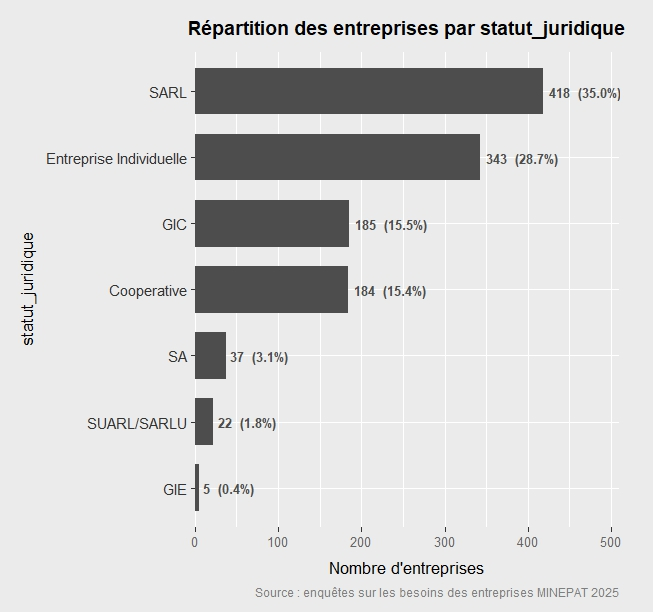
\includegraphics[width=0.75\textwidth]{statut.jpeg}
		\caption{Répartition des entreprises enquêtées par statut juridique}
		\label{fig:statut_juridique}
	\end{figure}
\newpage
	\subsubsection{Répartition des entreprises par région}
	Le Cameroun compte 10 régions et au vue des données exploitées, nous pouvons relevés une répartition assez inéquitable.
	En effet plus de la moitié des entreprises interrogées sont implentées dans les régions du Centre et du Littoral avec
	respectivement un pourcentage de 39,3\% et 17,8\%. Les autres régions se partagent 42,9\% avec les régions du Nord-Ouest et du Sud-Ouest qui ferment la marque avec respectivement 2,7\% et 2,8\% des entreprises étudiées. 
	\begin{figure}[H]
		\centering
		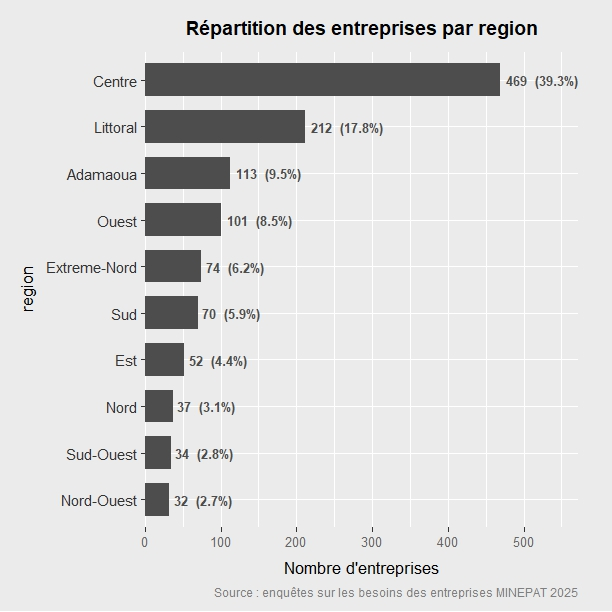
\includegraphics[width=0.75\textwidth]{repartition_region.jpeg}
		\caption{Répartition des entreprises enquêtées par région}
		\label{fig:region}
	\end{figure}
	
	
	
	\subsubsection{Répartition des entreprises par taille}
	La taille de l'entreprise repose sur le nombre de salariés et le chiffre d'affaires annuel de celle ci. %(https://blog.hubspot.fr/sales/taille-entreprise-classification)
	La discribution des entreprises par taille reflète la structure du tissus productif camerounais,
	caractérisé par une prédominance des petites entreprises et des très petites entreprises Les Grandes Entreprises sont très peu nombreuses et constituent 1,3\% des entreprises interrogées.
	\begin{figure}[H]
		\centering
		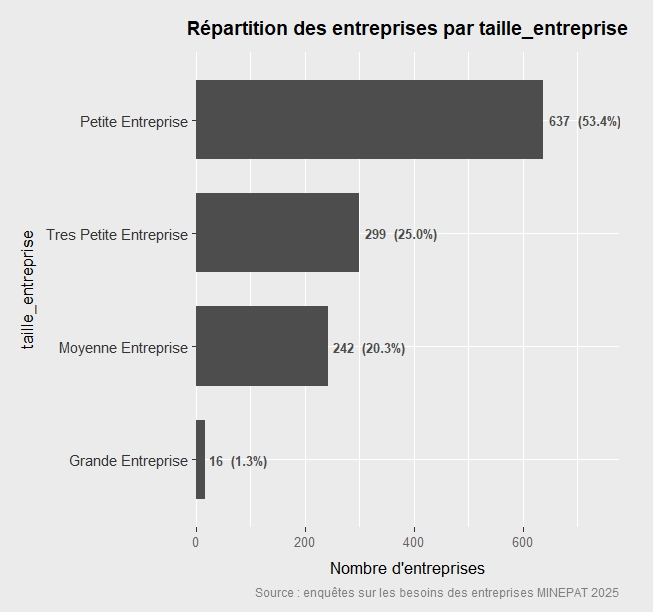
\includegraphics[width=0.75\textwidth]{repartition_taille.jpeg}
		\caption{Répartition des entreprises enquêtées par taille}
		\label{fig:taille}
	\end{figure}
	
	\subsubsection{Répartition des entreprises par ancienneté}
	La capacité d'une entreprise à se maintenir dans le temps témoigne de sa résilience et de sa force. 
	La répartition des entreprises par ancienneté indique que ce sont les entreprises de 5 à 9 ans
	d'ages qui ce sont le plus prétées au jeu avec 39,0\% de participation. Les entreprises ayant pas plus de 4  ans sont relativement nombreuses avec un pourcentage de 31,2\%. 
	\begin{figure}[H]
		\centering
		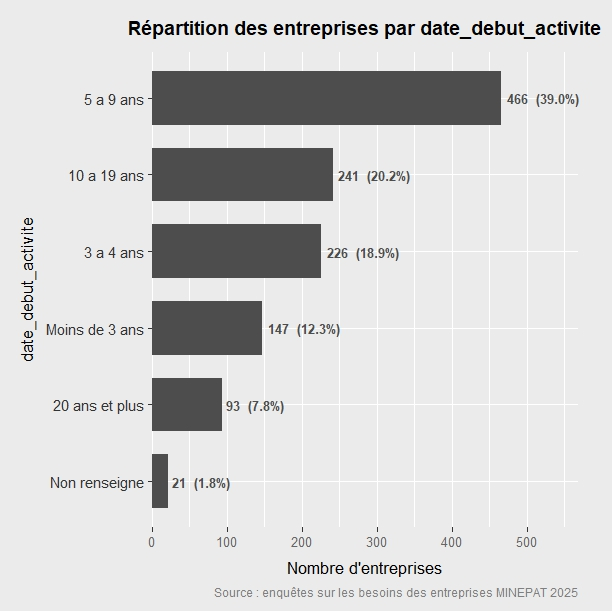
\includegraphics[width=0.75\textwidth]{anciennete.jpeg}
		\caption{Répartition des entreprises enquêtées par ancienneté}
		\label{fig:anciennete}
	\end{figure}
	
	
	\subsubsection{Répartition des entreprises par secteur d'activité}
	Les secteurs d'activités des entreprises locales sont plutot diversifiés. Nous avons pu relevé que 
le secteur de l'agriculture et de l'agroalimentaire est le plus représenté dans les entreprises locales, 
il détient à lui seul 62,6\% des entreprises étudiées. Les secteurs de l'industrie manufacturière et des 
Technologies de l'Informations et de la Communication sont assez peu nombreuses avec respectivement des taux de 5,2 \% et 3,7 \%. 
	\begin{figure}[H]
		\centering
		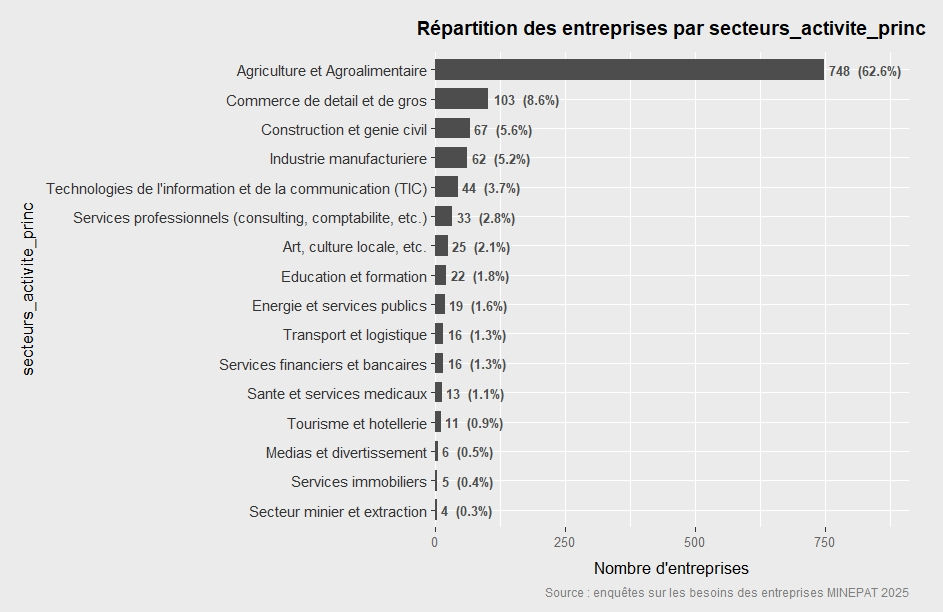
\includegraphics[width=0.75\textwidth]{repartition_activite.jpeg}
		\caption{Répartition des entreprises enquêtées par secteur d'activité}
		\label{fig:secteur}
	\end{figure}

	\subsubsection{Répartition des besoins exprimés}
	
	Les entreprises interrogées ont exprimé des besoins divers en relation avec les problèmes rencontrés quotidiennement. Le besoin qui revient le plus est celui du financement avec un taux de 20,1\% ce qui pourrait s'expliquer par une prédominance des TPE et des PME qui ont besoin de fonds pour une meilleur implentation. Vient ensuite le besoin en équipements avec 19,4\%, le besoin de transport est la moins fréquente ce qui traduirait l'existence d'infrastructures adéquat pour l'acheminement des produits.
	\begin{figure}[H]
		\centering
		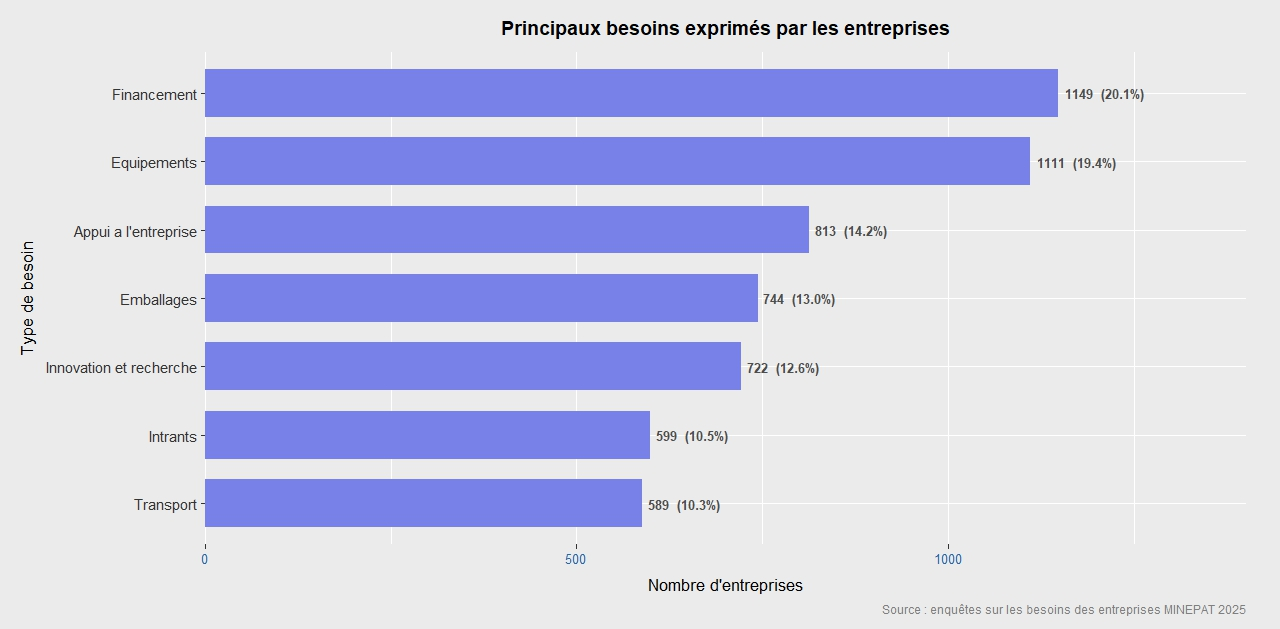
\includegraphics[width=0.75\textwidth]{repartition_besoins.jpeg}
		\caption{Répartition globale des besoins exprimés par les entreprises
			enquêtées}
		\label{fig:besoins_global}
		\end{figure}
			
			%-------------------------------------------------------------
			\subsection{Résultats de l'analyse bivariée}
			\label{subsec:bivariee}
			%-------------------------------------------------------------
			
			L'analyse bivariée a consisté à croiser les variables descriptives
			des entreprises avec les besoins qu'elles ont exprimés, afin
			d'identifier d'éventuelles associations structurelles entre les
			caractéristiques des entreprises et leurs besoins spécifiques. Deux
			outils ont été mobilisés~: les tableaux de contingence, qui permettent
			de visualiser la distribution conjointe des variables, et le test du
			$\chi^2$ de Pearson accompagné du coefficient $V$ de Cramér, qui
			permettent de tester et de quantifier l'intensité de ces associations
			\cite{saporta_2010}.
			
			\subsubsection{Répartition des besoins selon le statut juridique}
			
			Les figures ci-dessous présentent la distribution des besoins des
			entreprises selon leur statut juridique, ainsi que les résultats du
			test d'association correspondant.
			
			\begin{figure}[H]
				\centering
				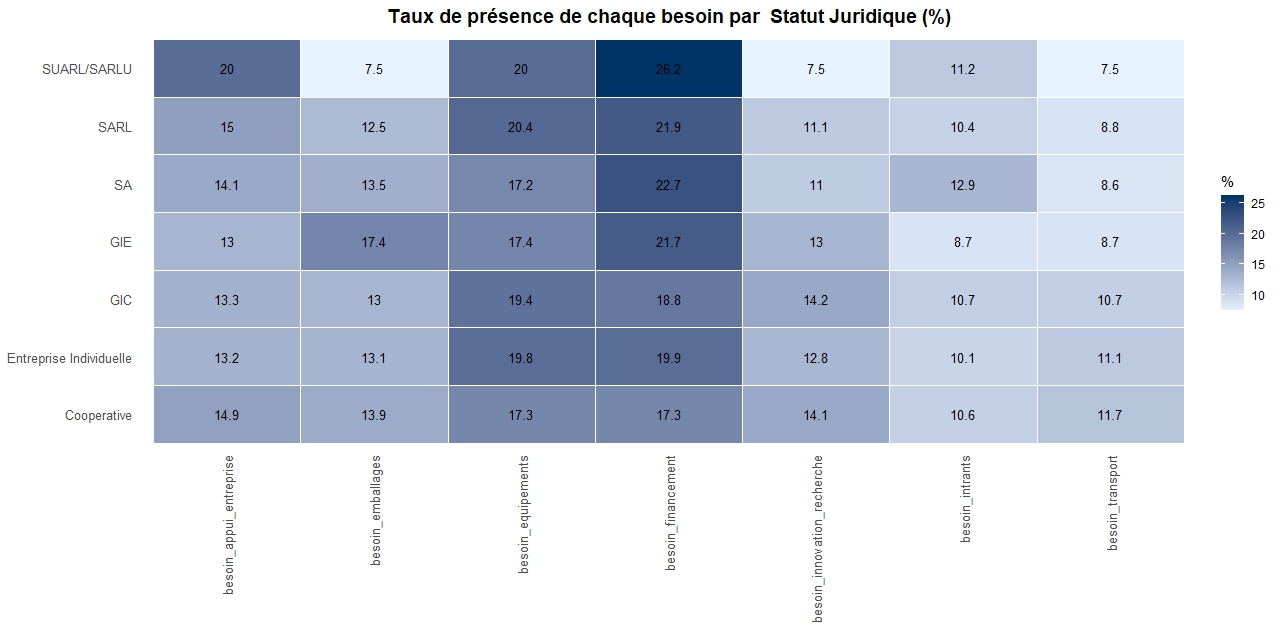
\includegraphics[width=\textwidth]{carte_chaleur_besoins_statut_juridique.jpeg}
				\caption{Distribution des besoins des entreprises selon le statut
					juridique}
				\label{fig:besoins_statut}
			\end{figure}
			
			\begin{table}[H]
				\centering
				\caption{Test du $\chi^2$ entre le statut juridique et les besoins
					des entreprises}
				\label{tab:khi2_statut}
				\renewcommand{\arraystretch}{1.4}
				\begin{tabularx}{\textwidth}{>{\raggedright\arraybackslash}X
						r r
						>{\centering\arraybackslash}p{2.8cm}
						r}
					\toprule
					\rowcolor{primary!15}
					\textbf{Besoin} & \textbf{$\chi^2$} & \textbf{p-valeur}
					& \textbf{Significatif} & \textbf{$V$ Cramér} \\
					\midrule
					Besoin en intrants        & 14,26 & 0,027  & Oui ($p < 0{,}05$) & 0,109 \\
					\rowcolor{lightgray}
					Besoin en financement     &  2,94 & 0,817  & Non                & 0,050 \\
					Besoin en emballages      & 44,47 & $<0{,}001$ & Oui ($p < 0{,}05$) & 0,193 \\
					\rowcolor{lightgray}
					Besoin en transport       & 50,44 & $<0{,}001$ & Oui ($p < 0{,}05$) & 0,206 \\
					Appui aux entreprises     & 26,32 & $<0{,}001$ & Oui ($p < 0{,}05$) & 0,148 \\
					\rowcolor{lightgray}
					Besoin en équipements     & 61,66 & $<0{,}001$ & Oui ($p < 0{,}05$) & 0,227 \\
					Innovation et recherche   & 77,88 & $<0{,}001$ & Oui ($p < 0{,}05$) & 0,255 \\
					\bottomrule
				\end{tabularx}
			\end{table}
			
			Les résultats du test du $\chi^2$ révèlent que le statut juridique
			est significativement associé à six des sept besoins étudiés, à
			l'exception du besoin en financement ($\chi^2 = 2{,}94$~;
			$p = 0{,}817$). Les associations les plus fortes concernent le besoin
			en innovation et en recherche ($V = 0{,}255$) et le besoin en
			équipements ($V = 0{,}227$), suggérant que la nature juridique de
			l'entreprise influence significativement la manière dont elle exprime
			ses besoins technologiques. Les entreprises de type SUARL/SARLU
			présentent notamment le taux le plus élevé de besoin en appui aux
			entreprises (20,0\,\%) et en financement (26,2\,\%), tandis que les
			Coopératives expriment davantage de besoins en innovation
			(14,1\,\%). Le besoin en financement constitue une exception notable~:
			il est exprimé de manière relativement homogène quelle que soit la
			forme juridique de l'entreprise, ce qui suggère que la contrainte
			financière est une réalité transversale à l'ensemble du tissu
			économique, indépendante du cadre juridique de l'entreprise.
			
			\subsubsection{Répartition des besoins selon la région}
			
			\begin{figure}[H]
				\centering
				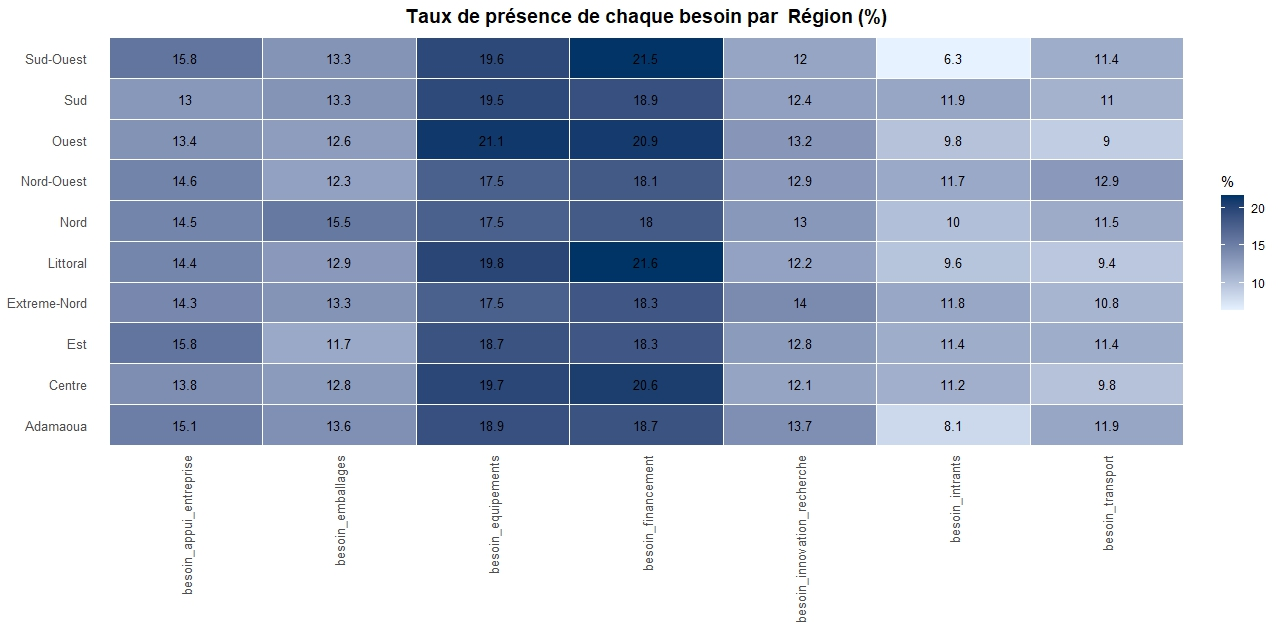
\includegraphics[width=\textwidth]{carte_chaleur_besoins_region.jpeg}
				\caption{Distribution des besoins des entreprises selon la région
					d'implantation}
				\label{fig:besoins_region}
			\end{figure}
			
			\begin{table}[H]
				\centering
				\caption{Test du $\chi^2$ entre la région d'implantation et les besoins
					des entreprises}
				\label{tab:khi2_region}
				\renewcommand{\arraystretch}{1.4}
				\begin{tabularx}{\textwidth}{>{\raggedright\arraybackslash}X
						r r
						>{\centering\arraybackslash}p{2.8cm}
						r}
					\toprule
					\rowcolor{primary!15}
					\textbf{Besoin} & \textbf{$\chi^2$} & \textbf{p-valeur}
					& \textbf{Significatif} & \textbf{$V$ Cramér} \\
					\midrule
					Besoin en intrants        & 28,91 & $<0{,}001$ & Oui ($p < 0{,}05$) & 0,156 \\
					\rowcolor{lightgray}
					Besoin en financement     &  6,21 & 0,718  & Non                    & 0,072 \\
					Besoin en emballages      & 18,69 & 0,028  & Oui ($p < 0{,}05$)    & 0,125 \\
					\rowcolor{lightgray}
					Besoin en transport       & 29,83 & $<0{,}001$ & Oui ($p < 0{,}05$) & 0,158 \\
					Appui aux entreprises     & 23,36 & 0,005  & Oui ($p < 0{,}05$)    & 0,140 \\
					\rowcolor{lightgray}
					Besoin en équipements     & 28,25 & $<0{,}001$ & Oui ($p < 0{,}05$) & 0,154 \\
					Innovation et recherche   & 23,77 & 0,005  & Oui ($p < 0{,}05$)    & 0,141 \\
					\bottomrule
				\end{tabularx}
			\end{table}
			
			La région d'implantation s'avère significativement associée à six
			besoins sur sept, le besoin en financement étant à nouveau le seul
			pour lequel aucune association significative n'est détectée
			($\chi^2 = 6{,}21$~; $p = 0{,}718$). Ce résultat confirme le
			caractère transversal de la contrainte financière, commune à
			l'ensemble des régions. Les besoins en transport ($V = 0{,}158$)
			et en intrants ($V = 0{,}156$) présentent les associations les plus
			fortes avec la région, ce qui est cohérent avec les disparités
			infrastructurelles importantes entre les régions camerounaises.
			Les régions du Nord-Ouest de l'Adamaoua et de l'Est, qui concentrent une part
			significative des entreprises à besoins en transport élevés,
			illustrent comment les contraintes géographiques et l'état des
			infrastructures conditionnent les priorités des entreprises locales.
			
			\subsubsection{Répartition des besoins selon l'ancienneté}
			
			\begin{figure}[H]
				\centering
				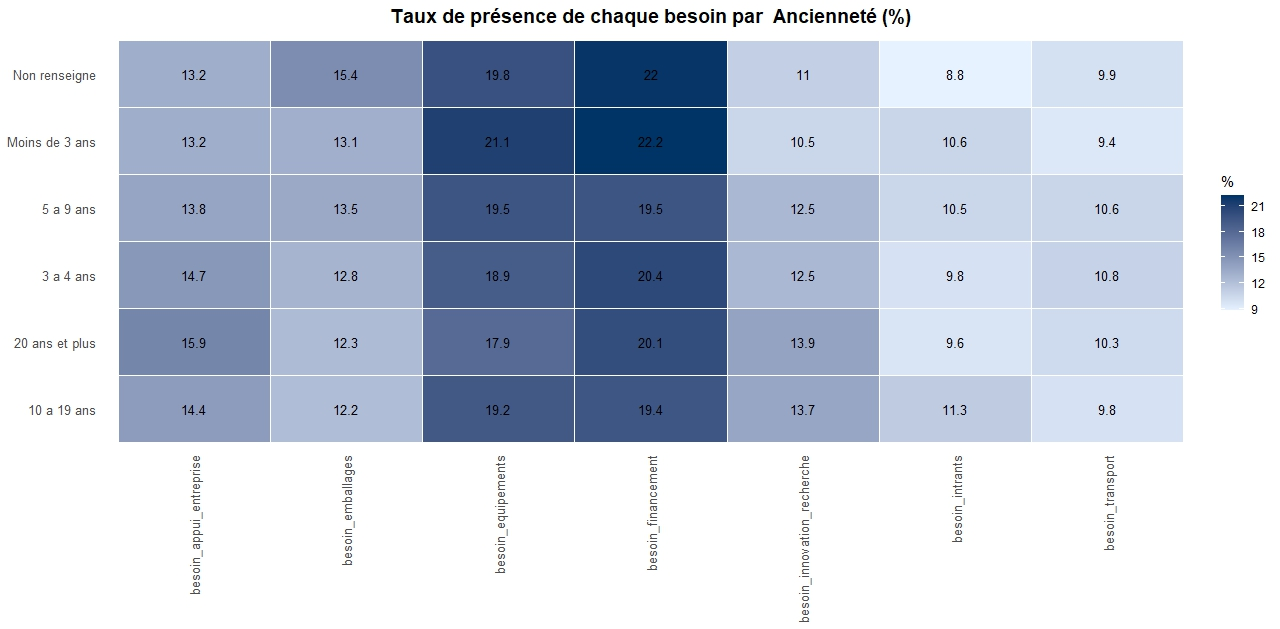
\includegraphics[width=\textwidth]{carte_chaleur_besoins_anciennete.jpeg}
				\caption{Distribution des besoins des entreprises selon leur
					ancienneté}
				\label{fig:besoins_anciennete}
			\end{figure}
			
			\begin{table}[H]
				\centering
				\caption{Test du $\chi^2$ entre l'ancienneté et les besoins
					des entreprises}
				\label{tab:khi2_anciennete}
				\renewcommand{\arraystretch}{1.4}
				\begin{tabularx}{\textwidth}{>{\raggedright\arraybackslash}X
						r r
						>{\centering\arraybackslash}p{2.8cm}
						r}
					\toprule
					\rowcolor{primary!15}
					\textbf{Besoin} & \textbf{$\chi^2$} & \textbf{p-valeur}
					& \textbf{Significatif} & \textbf{$V$ Cramér} \\
					\midrule
					Besoin en intrants        &  6,46 & 0,264  & Non                 & 0,074 \\
					\rowcolor{lightgray}
					Besoin en financement     &  4,44 & 0,488  & Non                 & 0,061 \\
					Besoin en emballages      &  5,09 & 0,405  & Non                 & 0,065 \\
					\rowcolor{lightgray}
					Besoin en transport       &  5,52 & 0,356  & Non                 & 0,068 \\
					Appui aux entreprises     & 11,84 & 0,037  & Oui ($p < 0{,}05$)  & 0,100 \\
					\rowcolor{lightgray}
					Besoin en équipements     & 14,84 & 0,011  & Oui ($p < 0{,}05$)  & 0,111 \\
					Innovation et recherche   & 20,10 & 0,001  & Oui ($p < 0{,}05$)  & 0,130 \\
					\bottomrule
				\end{tabularx}
			\end{table}
			
			L'ancienneté de l'entreprise est le critère présentant le moins
			d'associations significatives avec les besoins, puisque seulement
			trois besoins sur sept lui sont significativement liés. Les entreprises
			jeunes (moins de 3 ans) expriment davantage de besoins en financement
			(22,2\,\%) et en équipements (21,1\,\%), ce qui s'explique par leur
			stade de développement~: en phase de démarrage, l'accès aux
			ressources matérielles et financières constitue la contrainte
			prioritaire. À l'inverse, les entreprises plus matures (20 ans et
			plus) expriment un besoin en innovation et en recherche plus marqué
			(13,9\,\%), témoignant d'une préoccupation croissante pour la
			compétitivité à long terme et la modernisation technologique au fur
			et à mesure que l'entreprise se consolide.
			
			\subsubsection{Répartition des besoins selon le secteur d'activité}
			
			\begin{figure}[H]
				\centering
				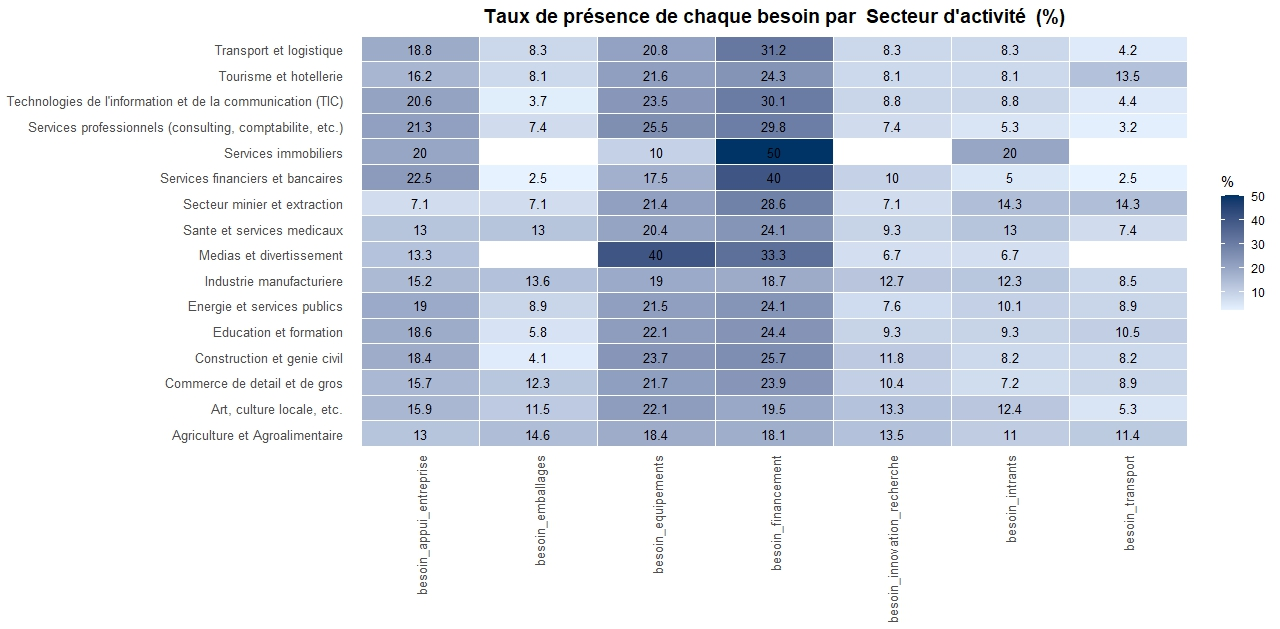
\includegraphics[width=\textwidth]{carte_chaleur_besoins_secteurs_activite.jpeg}
				\caption{Distribution des besoins des entreprises selon le secteur
					d'activité}
				\label{fig:besoins_secteur}
			\end{figure}
			
			\begin{table}[H]
				\centering
				\caption{Test du $\chi^2$ entre le secteur d'activité et les besoins
					des entreprises}
				\label{tab:khi2_secteur}
				\renewcommand{\arraystretch}{1.4}
				\begin{tabularx}{\textwidth}{>{\raggedright\arraybackslash}X
						r r
						>{\centering\arraybackslash}p{2.8cm}
						r}
					\toprule
					\rowcolor{primary!15}
					\textbf{Besoin} & \textbf{$\chi^2$} & \textbf{p-valeur}
					& \textbf{Significatif} & \textbf{$V$ Cramér} \\
					\midrule
					Besoin en intrants        & 103,48 & $<0{,}001$ & Oui ($p < 0{,}05$) & 0,294 \\
					\rowcolor{lightgray}
					Besoin en financement     &  34,10 & 0,003  & Oui ($p < 0{,}05$)    & 0,169 \\
					Besoin en emballages      & 306,81 & $<0{,}001$ & Oui ($p < 0{,}05$) & 0,507 \\
					\rowcolor{lightgray}
					Besoin en transport       & 147,87 & $<0{,}001$ & Oui ($p < 0{,}05$) & 0,352 \\
					Appui aux entreprises     &  20,13 & 0,167  & Non                    & 0,130 \\
					\rowcolor{lightgray}
					Besoin en équipements     & 239,10 & $<0{,}001$ & Oui ($p < 0{,}05$) & 0,447 \\
					Innovation et recherche   & 163,49 & $<0{,}001$ & Oui ($p < 0{,}05$) & 0,370 \\
					\bottomrule
				\end{tabularx}
			\end{table}
			
			Le secteur d'activité constitue la variable présentant les
			associations les plus fortes avec les besoins des entreprises~:
			six besoins sur sept lui sont significativement liés, avec des
			valeurs de $V$ de Cramér particulièrement élevées, notamment pour
			le besoin en emballages ($V = 0{,}507$), le besoin en équipements
			($V = 0{,}447$) et le besoin en transport ($V = 0{,}352$). Ces
			résultats confirment l'intuition selon laquelle le secteur d'activité
			est le principal déterminant de la nature des besoins exprimés par
			les entreprises. Les entreprises du secteur des Services immobiliers
			expriment le taux de besoin en financement le plus élevé (50,0\,\%),
			tandis que les entreprises du secteur des Médias et Divertissement
			présentent un besoin en équipements particulièrement fort (40,0\,\%).
			Le besoin en appui aux entreprises est le seul besoin pour lequel
			aucune association significative avec le secteur d'activité n'est
			détectée ($p = 0{,}167$), confirmant son caractère transversal à
			l'ensemble des secteurs.
			\subsubsection{Répartition des besoins selon la taille de l'entreprise}
			
			\begin{figure}[H]
				\centering
				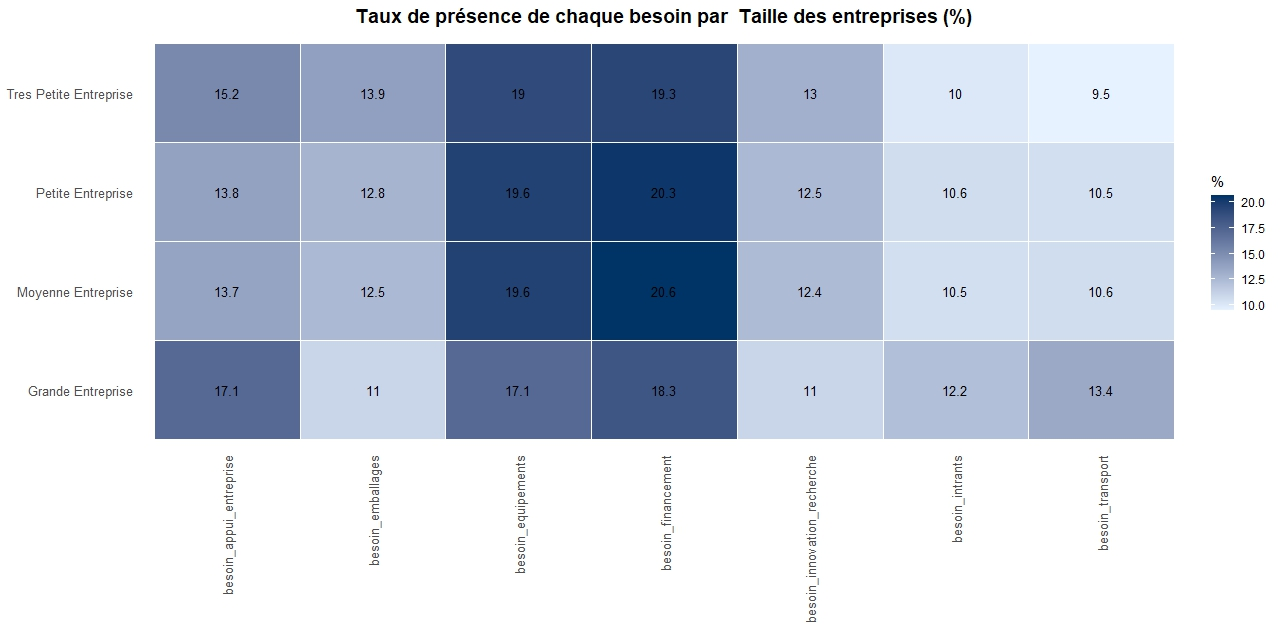
\includegraphics[width=\textwidth]{carte_chaleur_besoins_taille_entreprise.jpeg}
				\caption{Distribution des besoins des entreprises selon leur taille}
				\label{fig:besoins_taille}
			\end{figure}
			
			\begin{table}[H]
				\centering
				\caption{Test du $\chi^2$ entre la taille de l'entreprise et ses besoins}
				\label{tab:khi2_taille}
				\renewcommand{\arraystretch}{1.4}
				\begin{tabularx}{\textwidth}{>{\raggedright\arraybackslash}X
						r r
						>{\centering\arraybackslash}p{3cm}
						r}
					\toprule
					\rowcolor{primary!15}
					\textbf{Besoin} & \textbf{$\chi^2$} & \textbf{p-valeur}
					& \textbf{Significatif} & \textbf{$V$ Cramér} \\
					\midrule
					
					Besoin en intrants
					& 1,01 & 0,799 & Non & 0,029 \\
					
					\rowcolor{lightgray}
					Besoin en financement
					& 5,67 & 0,129 & Non & 0,069 \\
					
					Besoin en emballages
					& 7,48 & 0,058 & Non & 0,079 \\
					
					\rowcolor{lightgray}
					Besoin en transport
					& 3,20 & 0,362 & Non & 0,052 \\
					
					Besoin en appui aux entreprises
					& 13,95 & 0,003 & Oui ($p < 0{,}05$) & 0,108 \\
					
					\rowcolor{lightgray}
					Besoin en équipements
					& 2,25 & 0,521 & Non & 0,043 \\
					
					Innovation et recherche
					& 2,85 & 0,415 & Non & 0,049 \\
					
					\bottomrule
				\end{tabularx}
			\end{table}
			
			Les résultats du test du $\chi^2$ révèlent que la taille de
			l'entreprise n'est significativement associée qu'à un seul besoin sur
			les sept étudiés~: le besoin en appui aux entreprises ($\chi^2 =
			13{,}95$~; $p = 0{,}003$~; $V = 0{,}108$). Ce résultat est
			interprétable de manière intuitive~: les besoins d'accompagnement et
			d'appui institutionnel sont davantage ressentis par les petites
			structures, qui ne disposent pas en interne des ressources humaines
			et organisationnelles nécessaires pour gérer leurs activités de
			manière autonome, contrairement aux grandes entreprises qui
			internalisent généralement ces fonctions. L'association reste
			néanmoins modérée ($V = 0{,}108$), ce qui suggère que d'autres
			facteurs que la taille influencent également ce besoin.
			
			Pour les six autres besoins étudiés, aucune association
			statistiquement significative avec la taille de l'entreprise n'est
			détectée. Ce constat est particulièrement notable pour le besoin en
			financement ($\chi^2 = 5{,}67$~; $p = 0{,}129$), qui se confirme une
			nouvelle fois comme une contrainte universelle, indépendante de la
			taille de l'entreprise. De même, le besoin en équipements ($p =
			0{,}521$) et le besoin en innovation ($p = 0{,}415$) ne sont pas
			significativement liés à la taille, ce qui peut paraître surprenant
			mais s'explique par le fait que les besoins technologiques concernent
			l'ensemble des entreprises quel que soit leur niveau de développement,
			même si leur nature précise peut différer.
			
			
			
			
			%-------------------------------------------------------------
			\subsection{Résultats de l'analyse multidimensionnelle}
			\label{subsec:multi}
			%-------------------------------------------------------------
			
			Les analyses univariée et bivariée ont permis de décrire le tissu
			économique et d'identifier des associations entre les caractéristiques
			des entreprises et leurs besoins. Cependant, ces méthodes ne
			permettent pas d'appréhender simultanément l'ensemble des relations
			entre les variables dans leur globalité. L'analyse multidimensionnelle
			vient combler cette limite en offrant une représentation synthétique
			des données dans un espace factoriel de dimension réduite, à partir
			duquel des groupes d'entreprises aux profils similaires peuvent être
			construits et caractérisés. Elle s'articule en trois étapes
			successives~: l'ACM pour la réduction de dimension, la CAH pour
			la construction des classes, et l'AFD pour leur validation et
			caractérisation.
			
			\subsubsection{Analyse des Correspondances Multiples (ACM)}
			
			L'ACM a été conduite à l'aide du package \texttt{FactoMineR} du
			langage R %\cite{lebart_morineau_piron_1995}
			, sur l'ensemble des
			variables qualitatives retenues pour décrire les entreprises et
			leurs besoins. Son objectif principal est d'identifier les axes
			factoriels sur lesquels les données présentent la plus grande
			variabilité, afin de produire une représentation synthétique du
			nuage d'entreprises dans un espace de dimension réduit.
			
			\paragraph{Valeurs propres et inertie expliquée}
			
			Le choix du nombre d'axes à retenir s'effectue à partir de
			l'examen de l'éboulis des valeurs propres, qui représente la
			part d'inertie totale expliquée par chacun des axes factoriels.
			
			\begin{figure}[H]
				\centering
				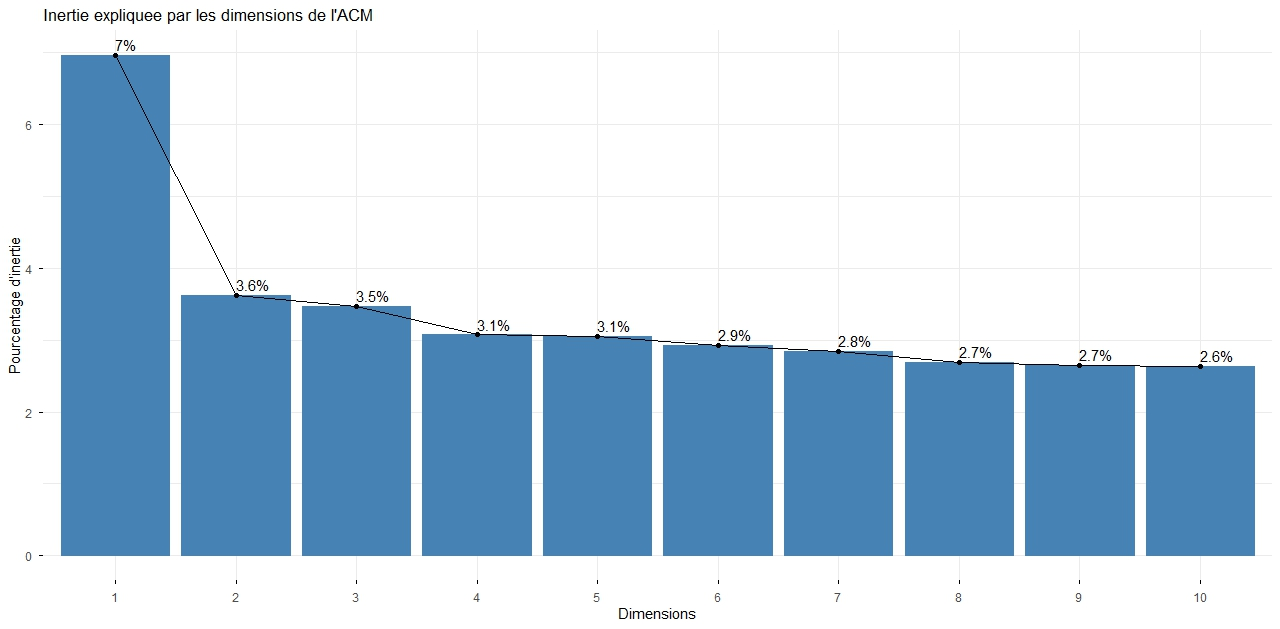
\includegraphics[width=0.75\textwidth]{contributionValeursPropres.jpeg}
				\caption{Éboulis des valeurs propres de l'ACM --- part d'inertie
					expliquée par axe factoriel}
				\label{fig:acm_vp}
			\end{figure}
			
			L’objectif principal de l’ACM étant l’interprétation à partir des projections des modalités sur les axes factoriels, le nombre d’axes à retenir est choisi en utilisant le critère du « coude »% (Cours Méthodes Factorielles Cnam UE).
			 Le critère du coude stipule que: (i) avant le coude, la pente est très raide. Chaque axe supplémentaire apporte une quantité importante d'information (d'inertie); (ii) après le coude, la courbe s'aplatit et forme un plateau linéaire. Les axes suivants n'apportent que du "bruit de fond" ou des détails négligeables. A partir de cette règle et de la figure \ref{fig:acm_vp} nous avons choisi les 5 premiers axes factoriels.
			
			
			\paragraph{Projection des modalités sur le premier plan factoriel}
		

			La projection des modalités sur les deux premiers axes factoriels
			permet de visualiser les associations entre les différentes modalités
			des variables et d'identifier les oppositions structurantes du nuage
			de points.
			
			\begin{figure}[H]
				\centering
				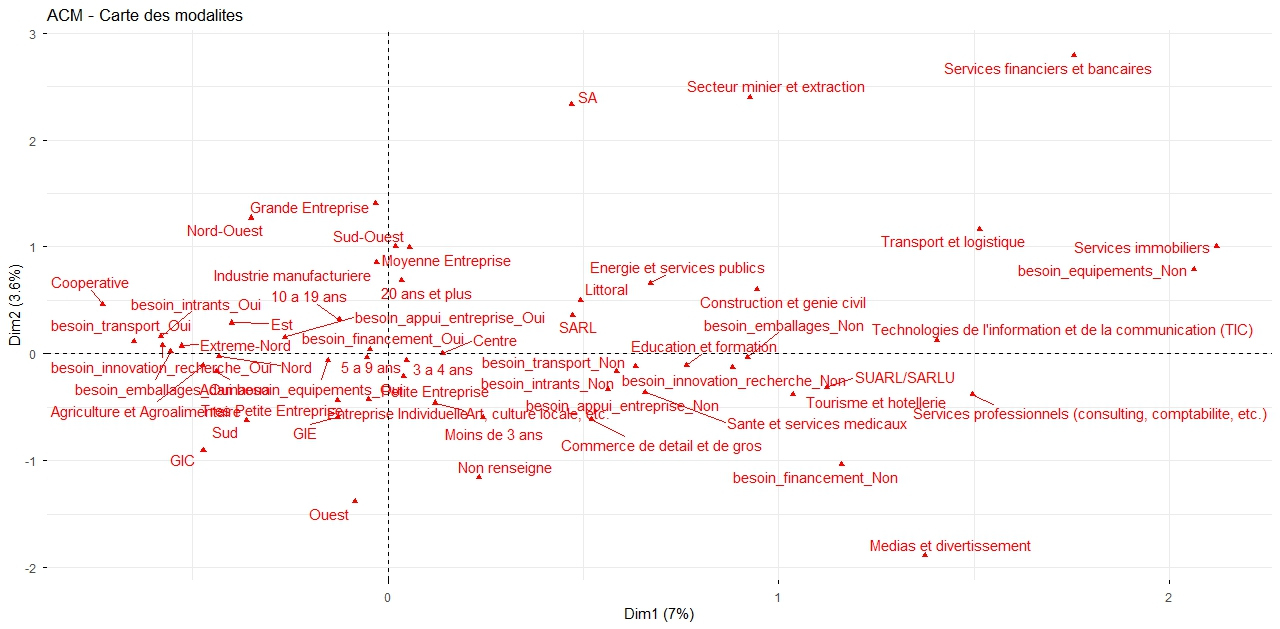
\includegraphics[width=\textwidth]{projectionDesCategories.jpeg}
				\caption{Projection des modalités sur le premier plan factoriel
					de l'ACM (axes 1 et 2)}
				\label{fig:acm_projection}
			\end{figure}
			
			On observe dans la figure \ref{fig:acm_projection} que bien de modalités sont assez proches des deux premiers axes factoriels. L'axe 1 oppose les entreprises tertiaires des entreprises du secteur primaire à travers la présence ou non d'un certains nombre de besoins et la répartition des secteurs d'activités. L'axe 2 permet de discriminer les statuts des entreprises et leurs tailles. On peut remarquer la présence quasi au centre du besoin en financement considéré comme un besoin transversal des entreprises.
			
			\paragraph{Variables contribuant aux axes factoriels}
			
			Les figures suivantes présentent les contributions des variables
			au premier et au second axe factoriel, permettant d'identifier
			les attributs les plus structurants de chaque dimension.
			
			\begin{figure}[H]
				\centering
				\begin{minipage}{0.48\textwidth}
					\centering
					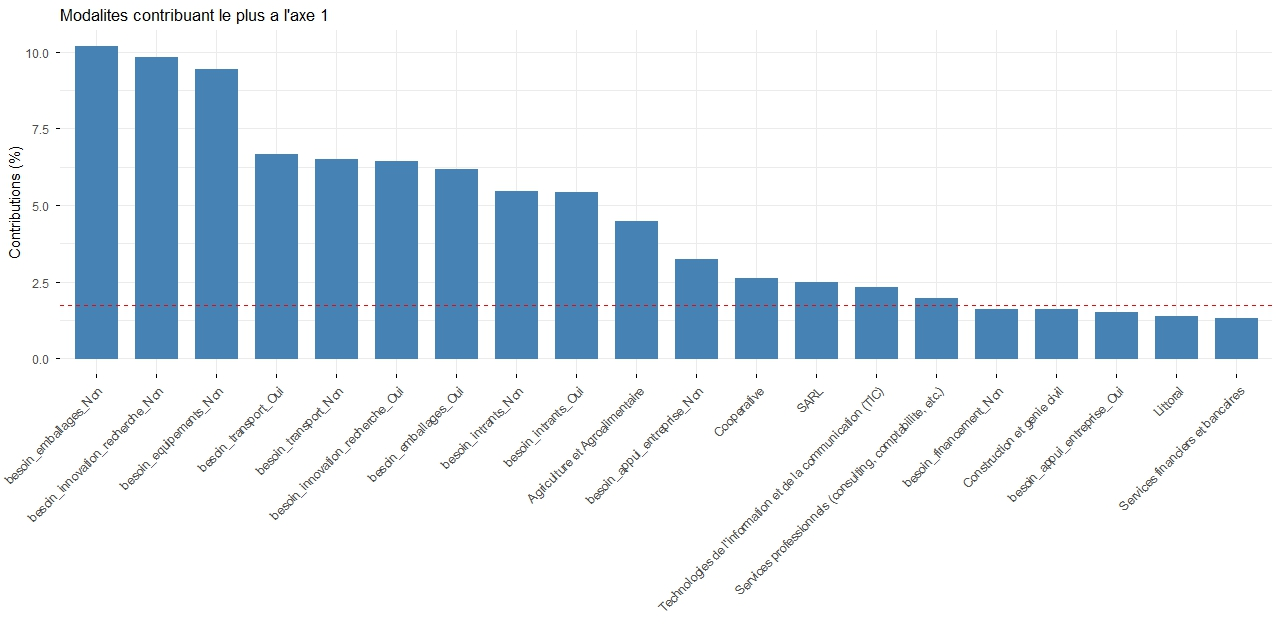
\includegraphics[width=\textwidth]{contributionCategoriesAlAxe1.jpeg}
					\caption{Contributions des modalités au premier axe factoriel}
					\label{fig:acm_contrib1}
				\end{minipage}
				\hfill
				\begin{minipage}{0.48\textwidth}
					\centering
					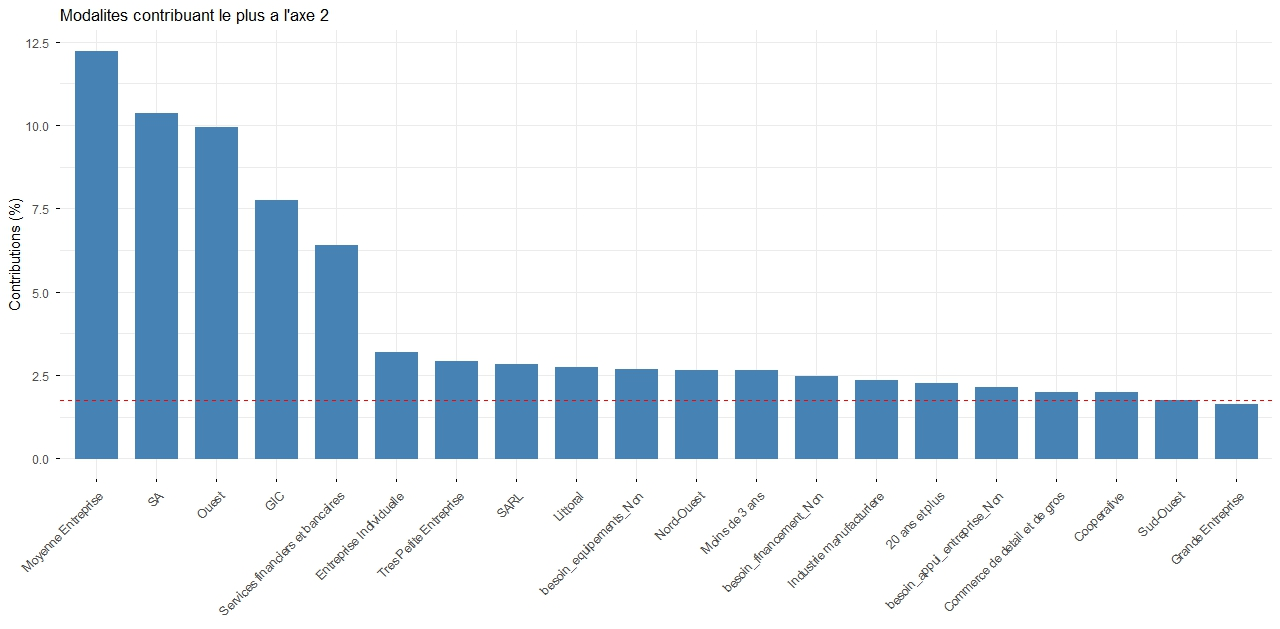
\includegraphics[width=\textwidth]{contributionCategorieALAxe2.jpeg}
					\caption{Contributions des modalités au second axe factoriel}
					\label{fig:acm_contrib2}
				\end{minipage}
			\end{figure}
			
		Le premier axe factoriel (Dim 1), qui capte la plus grande part de
		l'inertie de la structure des données (7\,\%), est fortement construit
		par des variables liées aux besoins opérationnels et techniques des
		structures. En observant l'éboulis des contributions, un groupe de
		trois modalités se détache très nettement au-dessus des autres,
		frôlant les 10\,\% de contribution chacune~:
		\texttt{besoin\_emballages\_Non},
		\texttt{besoin\_innovation\_recherche\_Non} et
		\texttt{besoin\_equipements\_Non}.
		Viennent ensuite, de manière équilibrée (entre 5\,\% et 7\,\%),
		les expressions contrastées des besoins logistiques et techniques
		(\texttt{besoin\_transport\_Oui},
		\texttt{besoin\_transport\_Non},
		\texttt{besoin\_innovation\_recherche\_Oui},
		\texttt{besoin\_emballages\_Oui}).
		Le seuil de contribution moyenne (ligne pointillée rouge à environ
		1{,}8\,\%) met en évidence que l'Axe~1 est presque exclusivement
		dicté par la dichotomie entre la présence et l'absence de besoins
		matériels et d'innovation au sein des structures.

		
		Le second axe factoriel (Dim 2, 3.6 \% de l'inertie) est quant à lui défini par des variables purement statutaires, institutionnelles et géographiques, marquant une rupture totale avec la logique de besoins de l'axe précédent. Le graphique des contributions montre que la construction de cet axe repose majoritairement sur cinq piliers qui dépassent de loin le seuil de contribution théorique : la taille moyenne d'entreprise (Moyenne Entreprise, ~12 \%), la forme juridique de Société Anonyme (SA, ~10.5 \%), la région de l'Ouest (~10 \%), le statut de Groupement d'Intérêt Communautaire (GIC, ~7.5 \%) et le secteur des Services financiers et bancaires (~6.5 \%). Les variables d'âge de l'entreprise ou de besoins opérationnels n'exercent ici qu'une influence très secondaire, ce qui confirme que l'Axe 2 capte spécifiquement le niveau de formalisation et de structuration légale des entités.
			
			\subsubsection{Classification Ascendante Hiérarchique (CAH)}
			
			La CAH a été conduite à partir des coordonnées factorielles des
			entreprises sur les axes retenus lors de l'ACM, en utilisant la
			méthode d'agrégation de Ward qui minimise la perte d'inertie
			inter-classes à chaque étape de fusion \cite{saporta_2010}. Cette
			approche, combinant ACM et CAH, est particulièrement adaptée aux
			données qualitatives dans la mesure où elle s'affranchit des
			problèmes liés aux distances euclidiennes calculées directement
			sur des variables catégorielles brutes.
			
			\paragraph{Dendrogramme et choix du nombre de classes}
			
			Le dendrogramme obtenu à l'issue de la CAH permet de visualiser
			la hiérarchie des regroupements.
			
			\begin{figure}[H]
				\centering
				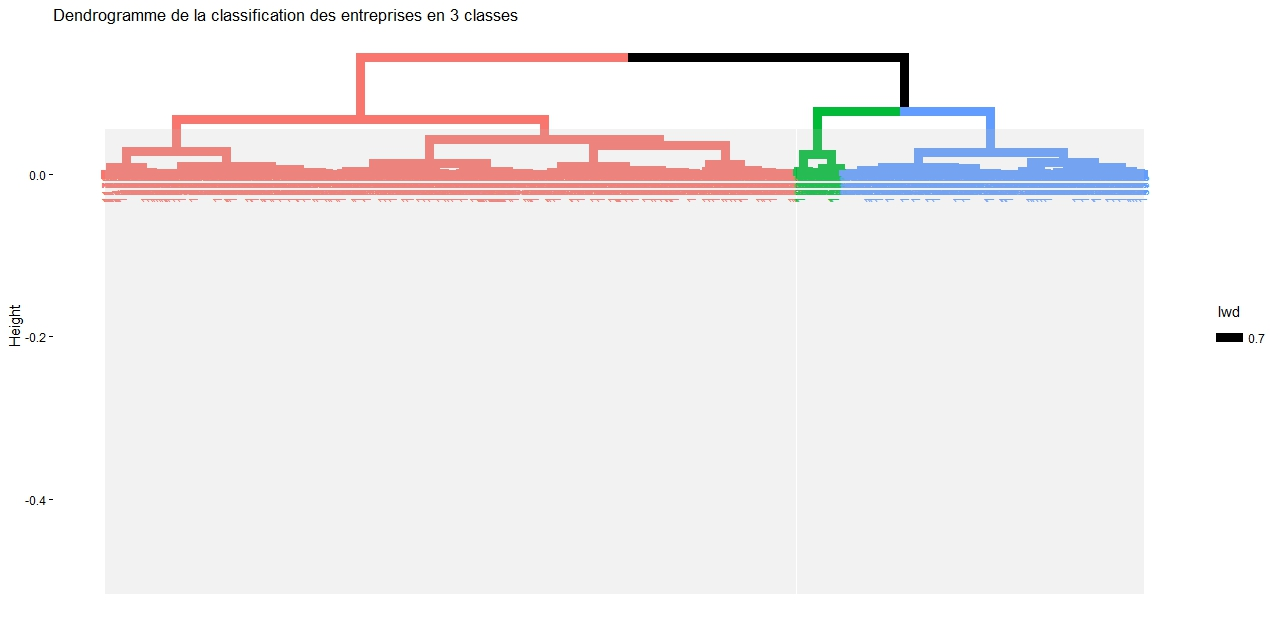
\includegraphics[width=0.85\textwidth]{dendrogramme.jpeg}
				\caption{Dendrogramme de la Classification Ascendante Hiérarchique
					(méthode de Ward)}
				\label{fig:dendrogramme}
			\end{figure}
			
			L'examen du dendrogramme (figure~\ref{fig:dendrogramme}) révèle
			l'existence d'un saut d'inertie particulièrement marqué à l'étape
			correspondant au passage de trois à deux classes, ce qui plaide en
			faveur d'une partition en \textbf{trois classes}. Ce choix est
			conforté par l'éboulis des indices de niveau, qui présente un
			décrochement net à ce niveau. La partition en trois classes offre
			par ailleurs une granularité suffisante pour identifier des profils
			d'entreprises distincts et opérationnellement utiles dans le cadre
			de l'algorithme de mise en relation de la plateforme.
			
			\paragraph{Visualisation de la partition obtenue}
			
			\begin{figure}[H]
				\centering
				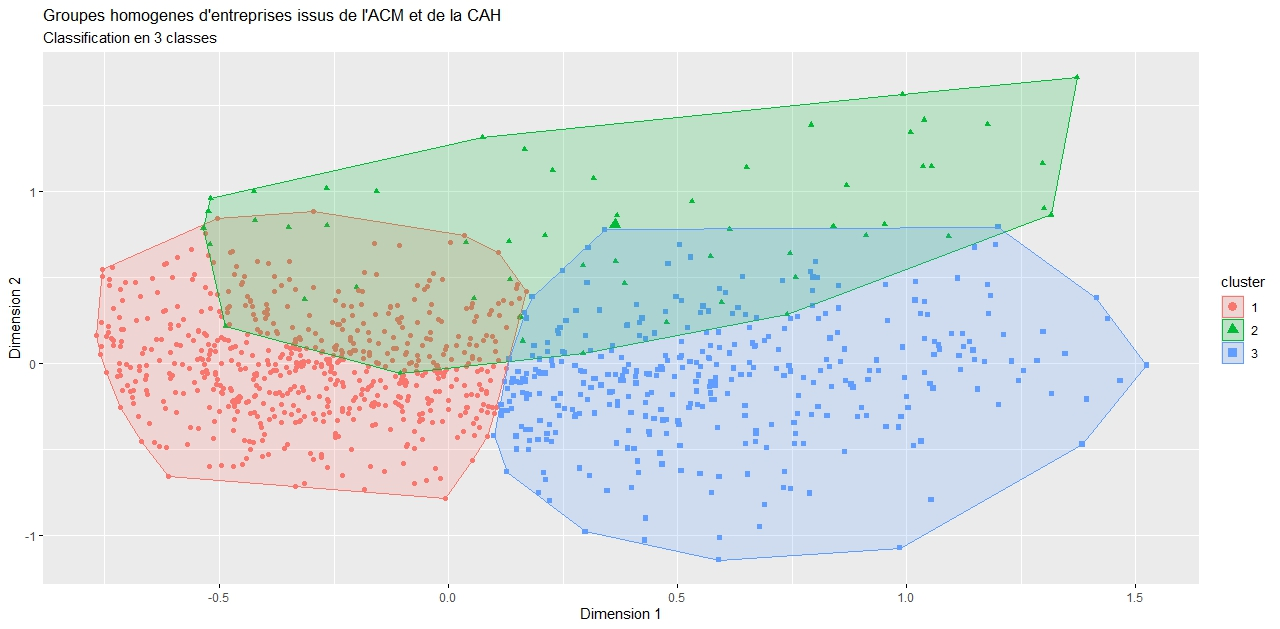
\includegraphics[width=\textwidth]{CAH.jpeg}
				\caption{Projection des trois classes obtenues par CAH sur le
					premier plan factoriel de l'ACM}
				\label{fig:cah_classes}
			\end{figure}
			
			La figure~\ref{fig:cah_classes} représente les trois classes
			d'entreprises obtenues, projetées sur le premier plan factoriel
			de l'ACM. La séparation visuelle des classes dans cet espace
			factoriel confirme la cohérence de la partition obtenue~: les
			trois groupes occupent des zones distinctes du plan factoriel,
			témoignant d'une bonne homogénéité intra-classe et d'une
			séparation satisfaisante inter-classes.
		
			\begin{itemize}
				\item \textbf{Classe 1} --- [753] entreprises (~63,1\,\%)~. L'on remarque que: (i) 40,2\% des entreprises de la classe 1 ont entre 5 et 9 ans d'anciennté; (ii)  
				81,1\% évolues dans le secteur de l'agriculture et de l'agroalimentaire; (iii) 36,3 \% sont dans la région du Centre; (iv) 52,5 \% sont des des petites entreprises. 
				\item \textbf{Classe 2} --- [57] entreprises (~4,8\,\%)~:
				profil dominant: (i) 26,4\% des entreprises ont plus de 20 ans; (ii) 54,4\% sont des Moyennes Entreprises; (iii) 45,5\% exercent leurs activités dans la région du centre; (iv) 24,6\% offrent des services financiers en bancaires.
				\item \textbf{Classe 3} --- [384] entreprises (~32,2\,\%)~:
				profil dominant: (i) 38,8\% ont entre 5 et 9 ans; (ii) 31,2\% sont dans le secteur de l'agriculture et de l'agroalimentaire; (iii) 45,6 \% sont implentés dans la région du centre et (iv) 59,6 \% sont des petites entreprises.
			\end{itemize}
			\begin{figure}[H]
				\centering
				\begin{minipage}{0.48\textwidth}
					\centering
					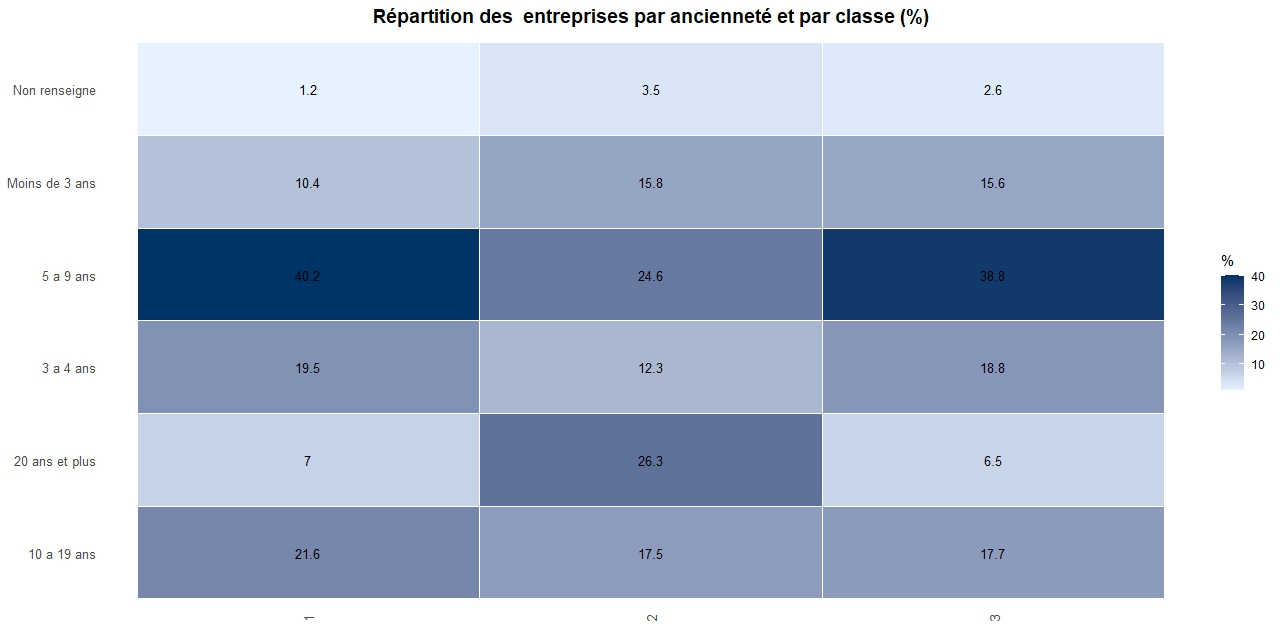
\includegraphics[width=\textwidth]{classe_et_anciennete.jpeg}
					\caption{Répartition des classes par ancienneté }
					\label{fig:rep_class_anc}
				\end{minipage}
				\hfill
				\begin{minipage}{0.48\textwidth}
					\centering
					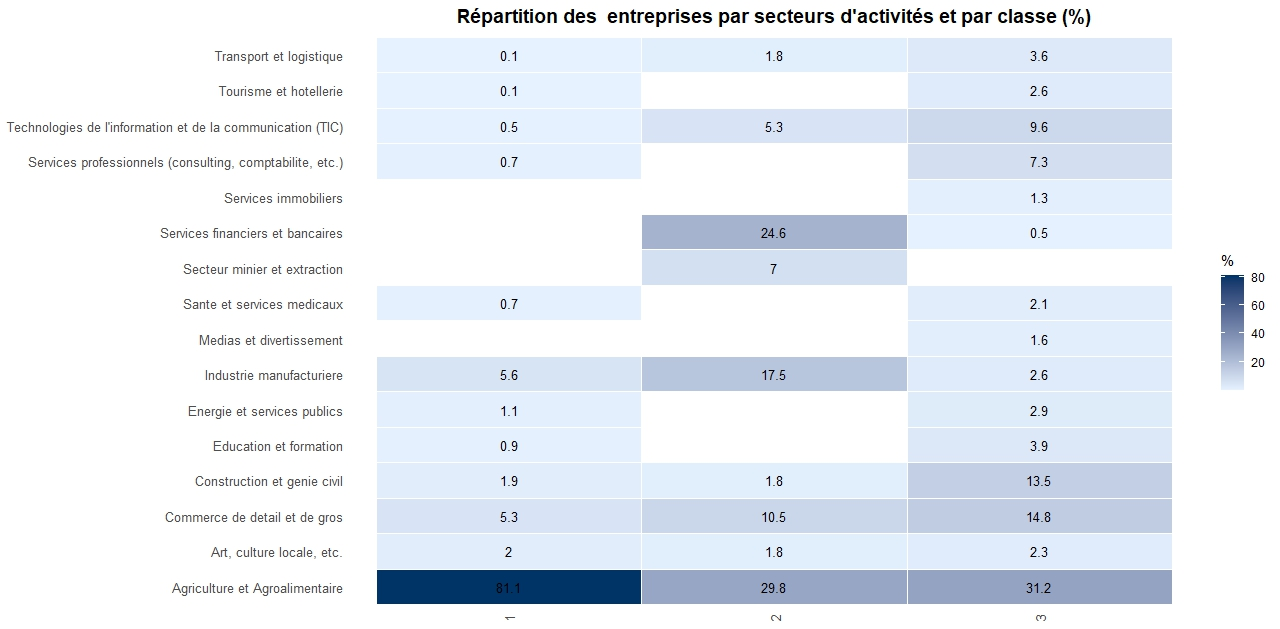
\includegraphics[width=\textwidth]{classes_et_secteurs_activites.jpeg}
					\caption{Répartition des classes par secteur d'activité}
					\label{fig:rep_classe_secteur}
				\end{minipage}
			\end{figure}
			\begin{figure}[H]
				\centering
				\begin{minipage}{0.48\textwidth}
					\centering
					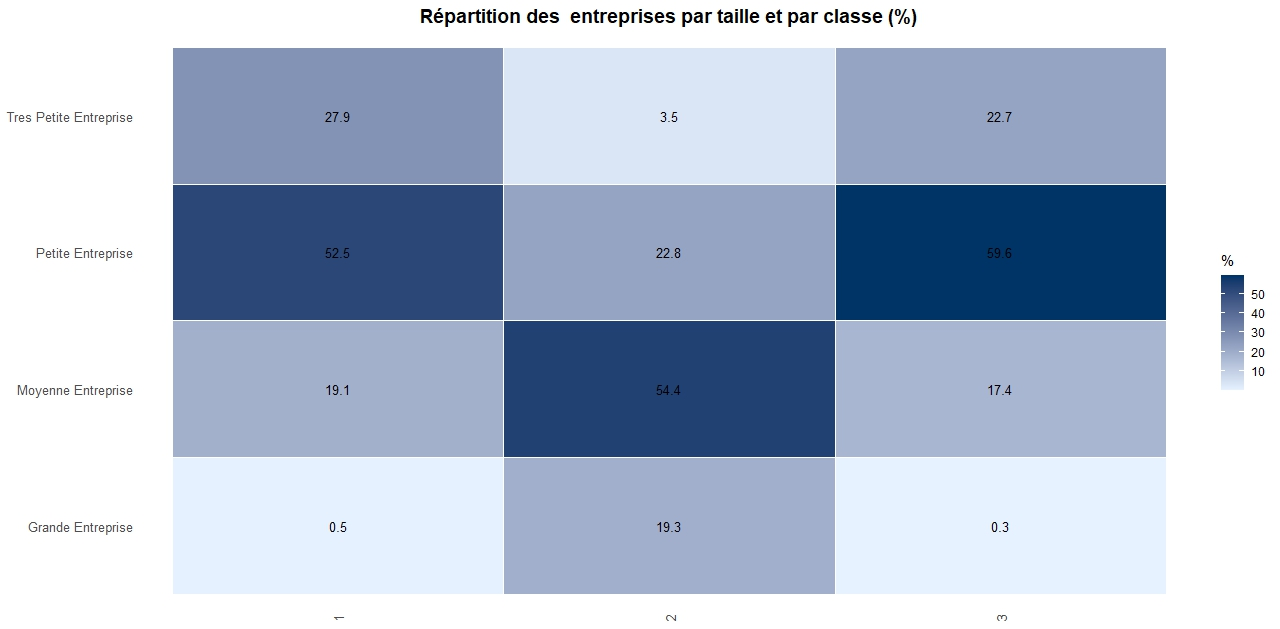
\includegraphics[width=\textwidth]{classes_et_tailles.jpeg}
					\caption{Répartition des classes par taille}
					\label{fig:rep_classe_taille}
				\end{minipage}
				\hfill
				\begin{minipage}{0.48\textwidth}
					\centering
					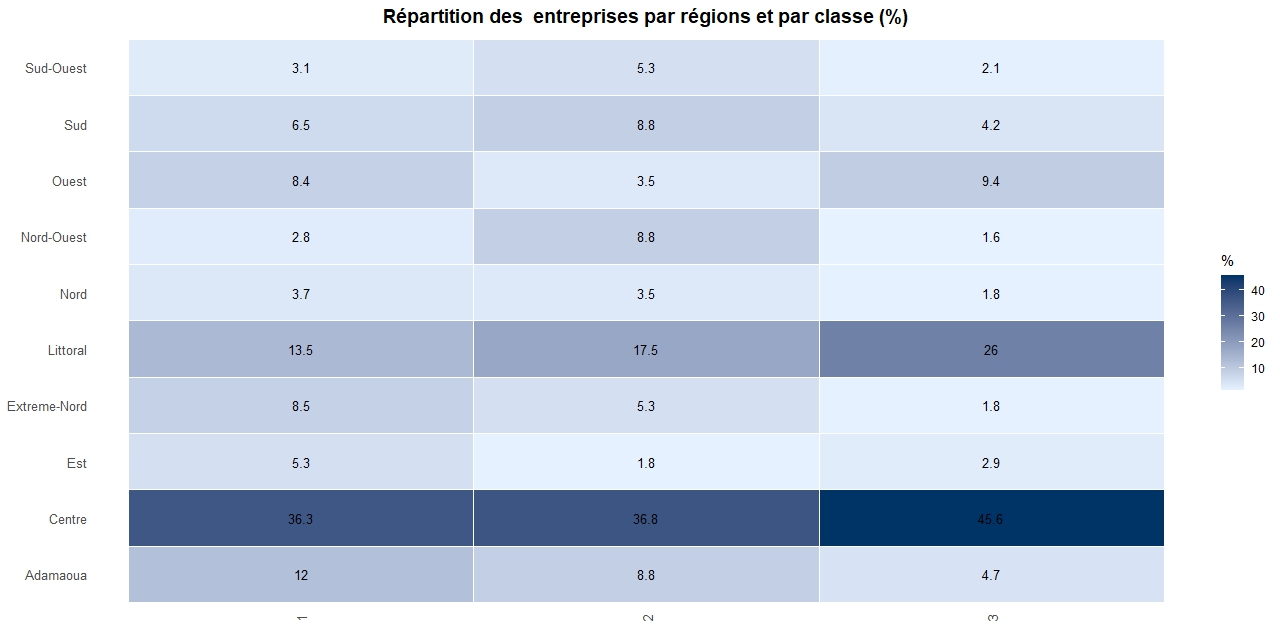
\includegraphics[width=\textwidth]{classes_et_regions.jpeg}
					\caption{Répartition des classes par région}
					\label{fig:rep_classe_region}
				\end{minipage}
			\end{figure}
			
			
			\subsubsection{Analyse Factorielle Discriminante (AFD)}
			
			L'AFD est conduite en aval de la CAH afin de valider la qualité de
			la partition obtenue et d'identifier les variables qui discriminent
			le mieux les trois classes d'entreprises \cite{saporta_2010}. Elle
			permet de répondre à deux questions complémentaires~: les classes
			identifiées sont-elles suffisamment distinctes pour être considérées
			comme des groupes homogènes~? Quelles variables permettent de les
			distinguer le plus efficacement~?
			
			\paragraph{Axes discriminants et pouvoir discriminant}
			
			\begin{figure}[H]
				\centering
				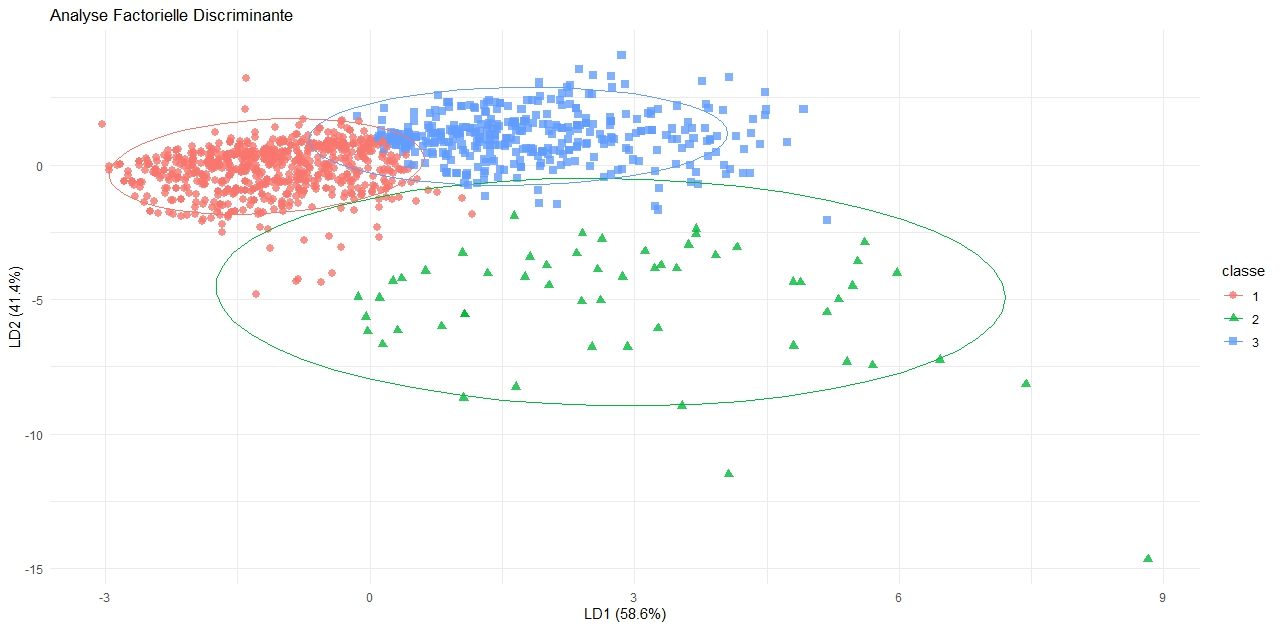
\includegraphics[width=0.85\textwidth]{AFDProjectionDesObservations.jpeg}
				\caption{Projection des entreprises et des centres de classes
					sur les axes discriminants de l'AFD}
				\label{fig:afd_projection}
			\end{figure}
			
			Le graphique de projection des observations met en évidence une excellente séparation globale des trois classes sur le plan formé par les deux premiers axes discriminants, qui captent ensemble 100 \% du pouvoir de séparation (58.6 \% pour LD1 et 41.4 \% pour LD2). Les ellipses de confiance à 95 \% confirment visuellement la pertinence statistique du modèle : bien qu'un léger chevauchement existe entre les classes 1 et 3, les trois nuages de points se structurent de manière distincte sans concentration massive au centre.
			
			
			\paragraph{Les axes factoriels obtenus}

L'Analyse Factorielle Discriminante (AFD) consiste à construire des combinaisons
linéaires des variables initiales --- appelées fonctions discriminantes canoniques ---
de manière à maximiser la variance inter-classes tout en minimisant la variance
intra-classes. Chaque axe obtenu (LD1, LD2, \ldots) représente ainsi une direction
de l'espace factoriel le long de laquelle les groupes issus de la Classification
Ascendante Hiérarchique (CAH) sont séparés de façon optimale. Les coefficients
associés à chaque variable sur ces axes, présentés dans le tableau~\ref{tab:variables_ld},
renseignent sur la contribution relative de chacune d'elles à la discrimination
entre les classes.
		
		\begin{table}[H]
			\centering
			\caption{Coefficients des variables sur les fonctions discriminantes canoniques}
			\label{tab:variables_ld}
			\renewcommand{\arraystretch}{1.4}
			\begin{tabularx}{\textwidth}{>{\raggedright\arraybackslash}X
					>{\centering\arraybackslash}p{3cm}
					>{\centering\arraybackslash}p{3cm}}
				\toprule
				\rowcolor{primary!15}
				\textbf{Variable} & \textbf{LD1} & \textbf{LD2} \\
				\midrule
				
				Dim1
				& 3,4117 & 0,8420 \\
				
				\rowcolor{lightgray}
				Dim2
				& 0,5020 & $-$2,8215 \\
				
				Dim3
				& 1,0018 & $-$2,3454 \\
				
				\rowcolor{lightgray}
				Dim4
				& 0,7551 & $-$2,1043 \\
				
				Dim5
				& $-$0,5523 & 1,0850 \\
				
				\bottomrule
			\end{tabularx}
		\end{table}
		
		
		
		% --- Commentaires analytiques (à intégrer dans le texte du mémoire) ---
		%
		 Le tableau~\ref{tab:variables_ld} présente les coefficients standardisés des variables
		 sur les deux premières fonctions discriminantes canoniques (LD1 et LD2).
		
		 \paragraph{Fonction LD1 — Axe de discrimination principal}
		 La première fonction discriminante est dominée par \textbf{Dim1} (coefficient = 3,41),
		 qui exerce la contribution la plus élevée en valeur absolue parmi toutes les variables.
		 Les variables Dim3 (1,00) et Dim4 (0,76) contribuent également positivement à LD1,
		 tandis que Dim5 présente une contribution négative modérée (--0,55). Dim2 (0,50) joue
		 un rôle secondaire sur cet axe. LD1 semble donc principalement structuré autour de
		 Dim1, qui peut être interprétée comme la dimension discriminante la plus puissante
		 entre les groupes.
		
		 \paragraph{Fonction LD2 — Axe secondaire de séparation}
		 La seconde fonction discriminante oppose fortement Dim2 (--2,82), Dim3 (--2,35)
		 et Dim4 (--2,10) aux variables Dim1 (0,84) et Dim5 (1,09), toutes deux à contribution
		 positive. LD2 capte ainsi une structure de variation orthogonale à LD1, permettant
		 d'affiner la séparation entre les groupes que LD1 ne distingue pas suffisamment.\\
		 
		 
		
		
		% ============================================================
		%  TABLEAU 2 — Indicateurs de performance du modèle
		% ============================================================
		
		
		Au-delà de la représentation factorielle, l'AFD poursuit un objectif de classification
		prédictive. À partir des fonctions discriminantes estimées, chaque observation est
		affectée à la classe dont le centroïde lui est le plus proche au sens de la distance
		de Mahalanobis, ce qui tient compte des corrélations entre variables et de la
		dispersion propre à chaque groupe. Les performances de ce modèle de classification
		sont évaluées à l'aide d'une matrice de confusion établie sur les données de test,
		dont les principaux indicateurs --- précision globale, indice Kappa de Cohen et
		tests de significativité --- sont consignés dans le tableau~\ref{tab:scores_modele}.
		\begin{table}[H]
			\centering
			\caption{Indicateurs de performance du modèle discriminant}
			\label{tab:scores_modele}
			\renewcommand{\arraystretch}{1.4}
			\begin{tabularx}{\textwidth}{>{\raggedright\arraybackslash}X
					>{\centering\arraybackslash}p{3.5cm}
					>{\centering\arraybackslash}p{3cm}}
				\toprule
				\rowcolor{primary!15}
				\textbf{Indicateur} & \textbf{Valeur} & \textbf{Interprétation} \\
				\midrule
				
				Accuracy
				& 0,9724 & Excellent \\
				
				\rowcolor{lightgray}
				Kappa de Cohen
				& 0,9435 & Accord quasi-parfait \\
				
				Accuracy Lower (IC 95\,\%)
				& 0,9614 & — \\
				
				\rowcolor{lightgray}
				Accuracy Upper (IC 95\,\%)
				& 0,9809 & — \\
				
				Accuracy Null
				& 0,6307 & Seuil classifieur naïf \\
				
				\rowcolor{lightgray}
				Accuracy P-value
				& $5{,}16 \times 10^{-183}$ & Hautement significatif \\
				
				McNemar P-value
				& $8{,}50 \times 10^{-7}$ & Significatif ($p < 0{,}05$) \\
				
				\bottomrule
			\end{tabularx}
		\end{table}
		
		% --- Commentaires analytiques (à intégrer dans le texte du mémoire) ---
		%
		 Le tableau~\ref{tab:scores_modele} synthétise les métriques d'évaluation du modèle
		 discriminant appliqué aux données de l'étude.
		
		 \paragraph{Précision globale (Accuracy)}
		 Le modèle affiche une précision globale de \textbf{97,24\,\%}, ce qui traduit un très
		 haut niveau de classification correcte des observations. L'intervalle de confiance à
		 95\,\% est étroit [96,14\,\% -- 98,09\,\%], confirmant la stabilité de cette estimation.
		
		 \paragraph{Indice Kappa de Cohen}
		 Le coefficient Kappa vaut \textbf{0,9435}, ce qui correspond à un accord quasi-parfait
		 entre les classes prédites et les classes réelles (seuil conventionnel : Kappa $> 0{,}80$
		 = très bon accord). Cet indicateur est particulièrement pertinent en présence de classes
		 déséquilibrées, car il corrige la précision en tenant compte du hasard.
		
		 \paragraph{Comparaison au classifieur naïf}
		 L'\textit{Accuracy Null} de 63,07\,\% représente la performance d'un classifieur trivial
		 attribuant systématiquement la classe majoritaire. Le gain de performance du modèle
		 par rapport à ce seuil est de $+34{,}17$ points de pourcentage, ce qui illustre
		 l'apport réel du modèle discriminant.
		
		 \paragraph{Significativité statistique}
		 La p-valeur associée à l'accuracy ($5{,}16 \times 10^{-183}$) est extrêmement faible,
		 rejetant sans ambiguïté l'hypothèse nulle selon laquelle le modèle ne serait pas meilleur
		 qu'un classifieur aléatoire. De même, le test de McNemar (p = $8{,}50 \times 10^{-7}$)
		 indique une asymétrie significative dans la matrice de confusion, suggérant que les
		 erreurs du modèle ne sont pas distribuées de façon uniforme entre les classes.
		
	
%=============================================================
\section{Présentation de la plateforme \textit{Business Partnership}}
\label{sec:presentation_plateforme}
%=============================================================

La présente section est consacrée à la présentation de la plateforme
\textit{Business Partnership}, fruit de l'ensemble des travaux de
conception et de développement décrits dans les chapitres précédents.
Elle expose successivement l'architecture de l'interface utilisateur,
les modalités d'implémentation de l'algorithme de mise en relation,
et les limites inhérentes à la solution développée. Cette présentation
s'appuie sur des captures d'écran de la plateforme dans son état
fonctionnel actuel, accompagnées de descriptions techniques précises
permettant d'apprécier la cohérence entre les exigences formulées
dans le cahier des charges et les réalisations effectives.

%-------------------------------------------------------------
\subsection{Architecture générale de la plateforme}
\label{subsec:architecture_generale}
%-------------------------------------------------------------

La plateforme \textit{Business Partnership} est une application web
développée selon le paradigme \textbf{MVT (Modèle-Vue-Template)}
proposé par le framework Django. Son architecture repose sur une
séparation claire entre trois couches fonctionnelles~: la couche
de présentation, qui assure le rendu des interfaces utilisateur via
les templates HTML et CSS~; la couche métier, qui contient la logique
applicative, le moteur de recommandation et les règles de gestion~;
et la couche de données, qui assure la persistance et la restitution
structurée des informations via l'ORM de Django et la base de données
SQLite. Cette architecture, représentée schématiquement à la
figure~\ref{fig:architecture_plateforme}, garantit une séparation
nette des responsabilités et facilite la maintenance évolutive de
la solution.

\begin{figure}[H]
	\centering
	\begin{tikzpicture}[
		layer/.style={rectangle, draw=primary, rounded corners=5pt,
			minimum width=11cm, minimum height=1.4cm,
			align=center, font=\small\bfseries},
		sublabel/.style={font=\small\color{darkgray}},
		arrow/.style={->, thick, color=primary}
		]
		\node[layer, fill=primary!15] (present) at (0, 0)
		{Couche Présentation \quad
			{\small\color{darkgray}(Templates HTML/CSS -- Bootstrap)}} ;
		
		\node[layer, fill=secondary!12] (metier) at (0, -2.2)
		{Couche Métier \quad
			{\small\color{darkgray}(Vues Django -- Logique applicative --
				Moteur de recommandation)}} ;
		
		\node[layer, fill=primary!8] (donnees) at (0, -4.4)
		{Couche Données \quad
			{\small\color{darkgray}(ORM Django -- SQLite --
				Coordonnées factorielles ACM)}} ;
		
		\draw[arrow] (present.south) -- (metier.north)
		node[midway, right, font=\tiny\color{darkgray}]
		{Requêtes HTTP} ;
		\draw[arrow] (metier.south) -- (donnees.north)
		node[midway, right, font=\tiny\color{darkgray}]
		{Requêtes ORM} ;
		\draw[arrow, bend right=40] (donnees.west)
		to node[left, font=\tiny\color{darkgray}] {Réponses}
		(present.west) ;
	\end{tikzpicture}
	\caption{Architecture en trois couches de la plateforme
		\textit{Business Partnership}}
	\label{fig:architecture_plateforme}
\end{figure}

%-------------------------------------------------------------
\subsection{Interface utilisateur}
\label{subsec:interface_utilisateur}
%-------------------------------------------------------------

L'interface utilisateur de la plateforme \textit{Business Partnership}
a été conçue selon les principes du design centré sur l'utilisateur,
en veillant à offrir une expérience de navigation intuitive, cohérente
et accessible, y compris pour des utilisateurs disposant d'une
familiarité limitée avec les outils numériques. L'ensemble des
composants visuels repose sur le framework CSS \textbf{Bootstrap},
qui garantit une cohérence graphique entre les différentes pages
de la plateforme et une adaptation automatique de l'interface
aux différentes tailles d'écran (\textit{responsive design}).
La charte graphique adoptée s'inspire de l'identité visuelle
institutionnelle du \gls{minepat}, avec une dominante de bleu
institutionnel et de blanc, afin de renforcer la légitimité
gouvernementale de la solution.

\subsubsection{Page d'accueil}

La page d'accueil constitue le premier point de contact entre
l'utilisateur et la plateforme. Elle a été conçue pour communiquer
de manière immédiate et claire la vocation de la plateforme, ses
fonctionnalités principales et les bénéfices qu'elle offre aux
entreprises. Elle comprend une bannière d'introduction présentant
les objectifs de la plateforme dans le cadre de la \gls{snd30},
un bloc de statistiques dynamiques affichant en temps réel le nombre
d'entreprises enregistrées, le nombre de besoins saisis et le nombre
de mises en relation initiées, ainsi qu'un appel à l'action invitant
les utilisateurs à créer leur compte ou à se connecter.

\begin{figure}[H]
	\centering
	\includegraphics[width=\textwidth]{./img/screenshot_accueil.png}
	\caption{Page d'accueil de la plateforme
		\textit{Business Partnership}}
	\label{fig:screen_accueil}
\end{figure}

\subsubsection{Tableau de bord de l'entreprise}

Le tableau de bord constitue l'espace de travail central de
l'utilisateur authentifié. Il offre une vue synthétique de l'état
du profil de l'entreprise, du nombre de besoins enregistrés, du
nombre de recommandations disponibles et des dernières mises en
relation initiées ou reçues. Un indicateur de complétude du profil,
exprimé en pourcentage, incite l'utilisateur à enrichir les
informations de son profil afin d'améliorer la pertinence des
recommandations générées en sa faveur. Ce tableau de bord est
organisé en modules indépendants accessibles depuis un menu de
navigation latéral persistant, garantissant une accessibilité
permanente aux différentes fonctionnalités de la plateforme en
un minimum de clics.

\begin{figure}[H]
	\centering
	\includegraphics[width=\textwidth]{./img/screenshot_dashboard.png}
	\caption{Tableau de bord de l'espace personnel d'une entreprise}
	\label{fig:screen_dashboard}
\end{figure}

\subsubsection{Formulaire de saisie des besoins}

Le formulaire de saisie des besoins a été conçu pour être à la fois
exhaustif et facile à compléter. Il propose une sélection parmi
les catégories de besoins identifiées lors de l'analyse statistique
(financement, équipements, intrants, transport, emballages, appui
institutionnel, innovation et recherche), accompagnée d'un champ
de description libre permettant à l'entreprise de préciser la
nature exacte de son besoin. Un menu déroulant permet de renseigner
le degré de priorité du besoin, tandis qu'un résumé des besoins
déjà enregistrés est affiché en bas de page, offrant à l'utilisateur
une vue consolidée de l'ensemble de ses besoins exprimés.

\begin{figure}[H]
	\centering
	\includegraphics[width=\textwidth]{./img/screenshot_besoins.png}
	\caption{Formulaire de saisie des besoins de l'entreprise}
	\label{fig:screen_besoins}
\end{figure}

\subsubsection{Page des recommandations}

La page des recommandations constitue la fonctionnalité à plus
forte valeur ajoutée de la plateforme. Elle présente à l'entreprise
une liste ordonnée des partenaires potentiels les plus compatibles
avec son profil, générée par le moteur de recommandation. Chaque
carte de recommandation affiche la raison sociale de l'entreprise
recommandée, son secteur d'activité, sa région d'implantation,
un résumé de ses besoins principaux, et le \textbf{score de
	compatibilité} calculé par l'algorithme, exprimé sous la forme
d'un indicateur visuel gradué. Un système de filtres permet à
l'utilisateur d'affiner les recommandations affichées selon des
critères géographiques, sectoriels ou relatifs à la taille de
l'entreprise, offrant ainsi une flexibilité d'exploration des
opportunités de partenariat.

\begin{figure}[H]
	\centering
	\includegraphics[width=\textwidth]{./img/screenshot_recommandations.png}
	\caption{Page de recommandations de partenaires potentiels}
	\label{fig:screen_recommandations}
\end{figure}

\subsubsection{Tableau de bord administrateur}

Le tableau de bord administrateur offre aux agents du \gls{minepat}
une vision panoramique et en temps réel de l'activité de la
plateforme. Il présente des indicateurs agrégés sur le nombre
d'entreprises enregistrées ventilées par région et par secteur,
le volume de besoins exprimés, le nombre de mises en relation
initiées et leur taux d'acceptation. Une section dédiée à la
gestion des demandes d'inscription en attente de validation permet
à l'administrateur de consulter, approuver ou rejeter chaque
demande après vérification des informations fournies. Un module
d'export permet de télécharger les données agrégées sous format
CSV à des fins d'analyses complémentaires.

\begin{figure}[H]
	\centering
	\includegraphics[width=\textwidth]{./img/screenshot_admin.png}
	\caption{Tableau de bord de l'espace administrateur}
	\label{fig:screen_admin}
\end{figure}

%-------------------------------------------------------------
\subsection{Implémentation de l'algorithme de mise en relation}
\label{subsec:implementation_algo}
%-------------------------------------------------------------

L'algorithme de mise en relation constitue le c\oe ur fonctionnel
différenciateur de la plateforme \textit{Business Partnership}
par rapport aux solutions existantes. Son implémentation repose
sur la chaîne analytique ACM~$\rightarrow$~CAH~$\rightarrow$
similarité cosinus, dont les étapes sont décrites ci-après.

\subsubsection{Préparation des données et projection dans
	l'espace factoriel}

La première étape de l'algorithme consiste à charger depuis la
base de données les coordonnées factorielles de chaque entreprise,
préalablement calculées lors de l'ACM conduite sur les données de
l'enquête du \gls{minepat}. Ces coordonnées, stockées dans la base
de données sous la forme de champs numériques associés à chaque
profil d'entreprise, représentent la projection de l'entreprise
dans l'espace factoriel réduit défini par les axes principaux de
l'ACM. Pour les entreprises nouvellement inscrites sur la plateforme,
dont les données n'étaient pas incluses dans l'enquête initiale,
une procédure de \textbf{projection supplémentaire} est appliquée~:
leurs coordonnées factorielles sont calculées en temps réel à partir
de la formule barycentrique de l'ACM, en utilisant les coordonnées
moyennes des modalités de leurs variables qualitatives.

\begin{lstlisting}[language=Python,
	caption={Projection d'une nouvelle entreprise dans l'espace
		factoriel de l'ACM}]
	def projeter_nouvelle_entreprise(profil: dict,
	coord_modalites: dict,
	nb_variables: int) -> list:
	"""
	Calcule les coordonnees factorielles d'une nouvelle entreprise
	par la formule barycentrique de l'ACM.
	profil           : dict {variable: modalite}
	coord_modalites  : dict {variable__modalite: [coord_axe1, ...]}
	nb_variables     : nombre de variables actives de l'ACM
	"""
	nb_axes = len(next(iter(coord_modalites.values())))
	coords  = [0.0] * nb_axes
	
	for variable, modalite in profil.items():
	cle = f"{variable}__{modalite}"
	if cle in coord_modalites:
	for s in range(nb_axes):
	coords[s] += coord_modalites[cle][s]
	
	# Division par le nombre de variables (formule barycentrique)
	return [c / nb_variables for c in coords]
\end{lstlisting}

\subsubsection{Calcul de la similarité cosinus}

La similarité entre deux entreprises $i$ et $j$ est calculée comme
le cosinus de l'angle formé par leurs vecteurs de coordonnées
factorielles dans l'espace de l'ACM. Cette mesure, comprise entre
$-1$ et $1$, est calculée pour chaque paire (entreprise cible,
entreprise candidate) et stockée temporairement en mémoire vive
pour la durée de la session de l'utilisateur, afin d'optimiser
les temps de réponse.

\begin{lstlisting}[language=Python,
	caption={Calcul de la similarité cosinus entre deux entreprises}]
	import numpy as np
	
	def similarite_cosinus(coords_i: list,
	coords_j: list) -> float:
	"""
	Calcule la similarite cosinus entre deux entreprises
	representees par leurs coordonnees factorielles.
	Retourne une valeur dans [-1, 1].
	"""
	vi = np.array(coords_i)
	vj = np.array(coords_j)
	
	norme_i = np.linalg.norm(vi)
	norme_j = np.linalg.norm(vj)
	
	if norme_i == 0 or norme_j == 0:
	return 0.0   # profil incomplet : similarite nulle
	
	return float(np.dot(vi, vj) / (norme_i * norme_j))
\end{lstlisting}

\subsubsection{Génération et classement des recommandations}

La fonction de génération des recommandations calcule la similarité
cosinus entre l'entreprise cible et l'ensemble des entreprises
enregistrées sur la plateforme, puis sélectionne et retourne les
$k$ entreprises présentant les scores de similarité les plus
élevés. Une contrainte d'exclusion est appliquée pour éviter qu'une
entreprise ne soit recommandée à elle-même, et un filtre optionnel
permet de restreindre les recommandations à un sous-ensemble
d'entreprises défini par des critères géographiques ou sectoriels
spécifiés par l'utilisateur.

\begin{lstlisting}[language=Python,
	caption={Génération des $k$ recommandations pour une entreprise}]
	def generer_recommandations(entreprise_id: int,
	entreprises: list,
	k: int = 5,
	filtre: dict = None) -> list:
	"""
	Retourne les k entreprises les plus similaires
	a l'entreprise cible (id = entreprise_id).
	entreprises : liste de dicts {id, coords, region, secteur}
	filtre      : dict optionnel {region: ..., secteur: ...}
	"""
	cible = next(e for e in entreprises
	if e['id'] == entreprise_id)
	scores = []
	
	for candidat in entreprises:
	if candidat['id'] == entreprise_id:
	continue
	# Application des filtres optionnels
	if filtre:
	if 'region' in filtre and \
	candidat['region'] != filtre['region']:
	continue
	if 'secteur' in filtre and \
	candidat['secteur'] != filtre['secteur']:
	continue
	
	score = similarite_cosinus(cible['coords'],
	candidat['coords'])
	scores.append({'entreprise': candidat,
		'score': round(score, 4)})
	
	# Tri decroissant par score et selection des k premiers
	scores.sort(key=lambda x: x['score'], reverse=True)
	return scores[:k]
\end{lstlisting}

\subsubsection{Intégration dans le cycle de vie Django}

L'algorithme de recommandation est intégré dans l'architecture
MVT de Django sous la forme d'un module Python indépendant
(\texttt{recommandation.py}), invoqué par la vue correspondante
lors de chaque accès à la page des recommandations. Cette
architecture modulaire garantit la séparation des responsabilités
entre la logique métier de recommandation et la logique de
présentation, et facilite les tests unitaires et les mises à
jour futures de l'algorithme sans impact sur le reste de
l'application. Le diagramme de séquence de la
figure~\ref{fig:sequence_algo} illustre le flux d'exécution
de l'algorithme lors d'une requête de recommandation.

\begin{figure}[H]
	\centering
	\begin{tikzpicture}[
		obj/.style={rectangle, draw=primary, fill=primary!10,
			minimum width=2.5cm, minimum height=0.7cm,
			align=center, font=\small\bfseries},
		msg/.style={->, thick, color=primary},
		ret/.style={dashed, ->, color=secondary},
		life/.style={dashed, color=darkgray, thick}
		]
		% Objets
		\node[obj] (user)   at (0, 0)    {Utilisateur};
		\node[obj] (vue)    at (3.5, 0)  {Vue Django};
		\node[obj] (algo)   at (7, 0)    {Module Reco};
		\node[obj] (db)     at (10.5, 0) {Base de données};
		
		% Lignes de vie
		\foreach \x in {0, 3.5, 7, 10.5}
		\draw[life] (\x, -0.35) -- (\x, -6.5);
		
		% Messages
		\draw[msg] (0,-0.8) -- (3.5,-0.8)
		node[midway,above,font=\tiny] {GET /recommandations/};
		\draw[msg] (3.5,-1.6) -- (10.5,-1.6)
		node[midway,above,font=\tiny] {Charger coordonnées entreprises};
		\draw[ret] (10.5,-2.4) -- (3.5,-2.4)
		node[midway,above,font=\tiny] {Liste coordonnées factorielles};
		\draw[msg] (3.5,-3.2) -- (7,-3.2)
		node[midway,above,font=\tiny] {generer\_recommandations(id, k=5)};
		\draw[msg] (7,-4.0) -- (7,-4.0);
		\node[font=\tiny, align=center] at (7,-4.2)
		{Calcul similarité\\cosinus ($\forall$ candidats)};
		\draw[ret] (7,-5.0) -- (3.5,-5.0)
		node[midway,above,font=\tiny] {Top-5 recommandations + scores};
		\draw[ret] (3.5,-5.8) -- (0,-5.8)
		node[midway,above,font=\tiny] {Rendu page recommandations};
	\end{tikzpicture}
	\caption{Diagramme de séquence du module de recommandation
		lors d'une requête utilisateur}
	\label{fig:sequence_algo}
\end{figure}

%-------------------------------------------------------------
\subsection{Évaluation des performances de la plateforme}
\label{subsec:evaluation_performances}
%-------------------------------------------------------------

L'évaluation des performances de la plateforme \textit{Business
	Partnership} porte sur deux dimensions complémentaires~: la qualité
algorithmique du moteur de recommandation, mesurée par les métriques
statistiques de classification issues de l'AFD~; et les performances
techniques de la plateforme, mesurées par les temps de réponse
observés lors des tests fonctionnels.

\subsubsection{Qualité du moteur de recommandation}

La qualité de l'algorithme de mise en relation repose directement
sur la qualité de la partition issue de la CAH, validée par l'AFD.
Le tableau~\ref{tab:perf_algo} présente les métriques de performance
du modèle de classification obtenues lors de la validation.

\begin{table}[H]
	\centering
	\caption{Métriques de performance du modèle de classification
		(validation par l'AFD)}
	\label{tab:perf_algo}
	\renewcommand{\arraystretch}{1.5}
	\begin{tabularx}{\textwidth}{>{\raggedright\arraybackslash}X
			>{\centering\arraybackslash}p{3.5cm}
			>{\raggedright\arraybackslash}X}
		\toprule
		\rowcolor{primary!15}
		\textbf{Métrique} & \textbf{Valeur} & \textbf{Interprétation} \\
		\midrule
		
		Accuracy (taux de bon classement)
		& 97,24\,\%
		& Excellent~: 97 entreprises sur 100 sont correctement
		affectées à leur classe \citep{lebart_morineau_piron_1995} \\
		
		\rowcolor{lightgray}
		Coefficient Kappa de Cohen
		& 0,9435
		& Accord quasi-parfait entre la classification prédite
		et la classification réelle (seuil $> 0{,}80$) \\
		
		Intervalle de confiance (95\,\%)
		& [96,14\,\%~; 98,09\,\%]
		& La performance est stable et significativement supérieure
		au seuil de 70\,\% préconisé dans la littérature \\
		
		\rowcolor{lightgray}
		Accuracy nulle (\textit{baseline})
		& 63,07\,\%
		& Performance d'un classifieur naïf attribuant toujours
		la classe majoritaire \\
		
		p-valeur (test de significativité)
		& $< 2{,}2 \times 10^{-16}$
		& La performance est hautement significative~; le modèle
		est nettement supérieur au hasard \\
		
		\rowcolor{lightgray}
		p-valeur (test de McNemar)
		& $8{,}50 \times 10^{-7}$
		& Les erreurs de classement ne sont pas symétriques,
		indiquant une discrimination différenciée selon les classes \\
		
		\bottomrule
	\end{tabularx}
\end{table}

Ces résultats attestent d'une qualité de classification
remarquable~: avec un taux de bon classement de \textbf{97,24\,\%}
et un coefficient Kappa de \textbf{0,9435}, le modèle d'AFD
valide avec une très forte robustesse la partition en classes
obtenue par la CAH. Ces performances constituent un indicateur
fort de la pertinence de l'algorithme de mise en relation de la
plateforme~: les entreprises d'une même classe présentent des
profils de besoins suffisamment homogènes pour que la similarité
cosinus calculée dans l'espace factoriel constitue un critère
de recommandation fiable et discriminant.

\subsubsection{Performances techniques}

Les tests fonctionnels conduits sur la plateforme ont permis de
mesurer les temps de réponse associés aux principales opérations.
L'ensemble des opérations respecte les seuils définis dans le
cahier des charges~: les pages de consultation de profils et
d'affichage des recommandations répondent en moins de 3 secondes,
et le calcul du Top-5 des recommandations pour une base de
1\,194 entreprises s'effectue en moins de 2 secondes, validant
ainsi l'adéquation de la solution aux contraintes de performance
fixées.

%-------------------------------------------------------------
\subsection{Limites du travail}
\label{subsec:limites}
%-------------------------------------------------------------

Tout travail scientifique et technique est sujet à des limites
qu'il convient d'identifier avec rigueur et honnêteté intellectuelle,
afin d'en délimiter clairement le champ de validité et d'en guider
les développements ultérieurs. Les limites du présent travail se
situent à trois niveaux distincts~: les limites relatives aux données,
les limites algorithmiques et les limites techniques.

\subsubsection{Limites relatives aux données}

La principale limite du travail tient à la nature et à la
représentativité des données exploitées. L'enquête du \gls{minepat}
de 2025, bien qu'ayant permis de collecter des informations sur
\textbf{1\,194 entreprises}, ne constitue pas un échantillon
probabiliste représentatif de l'ensemble du tissu productif
camerounais, évalué à plusieurs centaines de milliers d'unités
économiques par le RGE3 de l'INS \citep{ins_rge_2023}. La
sélection des entreprises enquêtées a reposé sur les réseaux
des délégués régionaux et départementaux du \gls{minepat}, ce
qui peut avoir introduit un biais de sélection en faveur des
entreprises disposant d'un accès à internet et d'une certaine
visibilité institutionnelle. Les entreprises du secteur informel
et les microentreprises rurales, qui représentent pourtant une
fraction importante du tissu économique national, sont probablement
sous-représentées dans l'échantillon. Cette limitation affecte
directement la généralisation des résultats de l'analyse statistique
et la représentativité du moteur de recommandation.

Par ailleurs, les données étant issues d'une enquête ponctuelle,
elles reflètent une photographie statique des besoins des entreprises
à un instant donné. Or, les besoins des entreprises évoluent dans
le temps en fonction des conjonctures économiques et des dynamiques
sectorielles. L'absence d'un mécanisme de mise à jour périodique
et automatisée des coordonnées factorielles de l'ACM constitue
donc une limite à la pérennité de la pertinence des recommandations
générées.

\subsubsection{Limites algorithmiques}

Sur le plan algorithmique, la similarité cosinus calculée dans
l'espace factoriel de l'ACM présente l'avantage d'être simple
à implémenter et rapide à calculer, mais ne capture pas l'ensemble
de la complexité des facteurs qui déterminent la compatibilité
entre deux entreprises. Elle repose en effet sur l'hypothèse que
la proximité dans l'espace factoriel est un proxy valide de la
complémentarité des besoins, ce qui peut ne pas être vérifié dans
tous les cas. Des approches plus sophistiquées, telles que les
systèmes de recommandation basés sur le filtrage collaboratif
(\textit{collaborative filtering}) ou les modèles de représentation
appris par des réseaux de neurones (\textit{embedding-based
	recommendation}), pourraient potentiellement offrir des
recommandations plus précises et contextuellement pertinentes,
au prix d'une complexité algorithmique et computationnelle
sensiblement plus élevée.

De plus, le moteur de recommandation actuel ne prend pas en compte
l'historique des interactions entre entreprises~: une mise en
relation refusée par une entreprise ne modifie pas les
recommandations futures, et aucun mécanisme d'apprentissage
à partir des retours utilisateurs n'a été implémenté dans cette
première version. L'intégration d'un tel mécanisme constitue
une piste d'amélioration majeure pour les versions futures.

\subsubsection{Limites techniques}

Sur le plan technique, la base de données SQLite retenue pour
cette version de développement présente des limitations de
performance et de concurrence qui la rendent inadaptée à un
déploiement en production à large échelle. La migration vers
un système de gestion de bases de données plus robuste, tel que
PostgreSQL, constitue un prérequis indispensable avant tout
déploiement opérationnel de la plateforme au sein du \gls{minepat}.

Par ailleurs, la plateforme ne dispose pas encore d'une couche
de cache (\textit{caching layer}) permettant de mémoriser les
résultats de recommandations déjà calculés, ce qui implique un
recalcul intégral de la similarité cosinus pour l'ensemble des
entreprises à chaque requête. Si cette approche est acceptable
pour une base de 1\,194 entreprises, elle pourrait induire des
dégradations de performance significatives lors d'un passage à
l'échelle impliquant plusieurs dizaines de milliers d'entreprises.
L'implémentation d'un mécanisme de cache distribué, par exemple
via Redis, est envisagée comme amélioration prioritaire pour la
version de production.

Enfin, la plateforme ne propose pas encore de version en langue
anglaise, ce qui limite son accessibilité aux entreprises des
régions anglophones du Cameroun, pourtant fortement représentées
dans le tissu économique national. La mise en place d'une
internationalisation complète de l'interface (\textit{i18n})
constitue une exigence \textit{Could have} identifiée dans le
cahier des charges, dont la réalisation est prévue dans une
version ultérieure.

\begin{remarque}
	Les limites identifiées dans cette section ne remettent pas en
	cause la validité et la pertinence de la solution développée dans
	le cadre de ce travail~: elles en délimitent le champ de validité
	actuel et tracent une feuille de route précise pour les développements
	futurs. La plateforme \textit{Business Partnership}, dans son état
	actuel, constitue un prototype fonctionnel qui démontre la
	faisabilité technique et la pertinence algorithmique de l'approche
	retenue, et pose les fondements d'une solution opérationnelle qui
	pourra être progressivement enrichie et déployée à plus grande
	échelle sous la supervision du \gls{minepat}.
\end{remarque}
	
	\subsection{Perspectives}
	
	
	
	%============================================================
	%  CONCLUSION GÉNÉRALE
	%============================================================
	\chapter*{Conclusion Générale}
	\addcontentsline{toc}{chapter}{Conclusion Générale}
	\markboth{Conclusion Générale}{Conclusion Générale}
	
	
	\medskip
	

	%============================================================
	%  BIBLIOGRAPHIE
	%============================================================
	%\printbibliography[heading=bibintoc, title={Bibliographie}]
\newpage
\bibliographystyle{plainnat}
\bibliography{references.bib} % Indiquez le nom de votre fichier .bib sans l'extension
%\printbibliography[title={Bibliographie}] % Génère la liste des références
	%============================================================
	%  ANNEXES
	%============================================================
	\appendix
	\chapter{Questionnaire de l'enquête MINEPAT 2025}
	\label{ann:questionnaire}
	
	
	
	\chapter{Modèle de données complet}
	\label{ann:modele}
	
	
	
	\chapter{Manuel d'utilisation de la plateforme}
	\label{ann:manuel}
	

	
	
\end{document}